\documentclass[11pt]{article}

\usepackage[margin=1in]{geometry}
\usepackage{graphicx}
\usepackage{booktabs}
\usepackage{amsmath,amssymb}
\usepackage{natbib}
\usepackage{hyperref}
\usepackage{xcolor}
\usepackage{multirow}
\usepackage{caption}
\usepackage{subcaption}
\usepackage{enumitem}
\usepackage{microtype}
\usepackage{url}

\setcounter{topnumber}{3}
\setcounter{totalnumber}{4}
\renewcommand{\topfraction}{0.9}
\renewcommand{\textfraction}{0.07}
\renewcommand{\floatpagefraction}{0.8}

\title{Semantic Drift Across Qwen Generations:\\
Reproducibility, Thinking Mode, Serving Stack, and What Cosine Similarity
Misses in Iterated Paraphrase Chains}

\author{
  James H.\ Smith \\
  Joshua.AI LLC \\
  \texttt{jim@joshua8.ai}
}

\date{September 2026}

\begin{document}
\maketitle

\begin{abstract}
We extend the telephone-game study of semantic drift in iterated LLM
paraphrase chains~\citep{smith2026drift} to the Qwen3.6 and Qwen3.8 model
generations, and we use the fast, cheap inference these models afford to ask
questions the earlier work could not: whether a sampling seed reproduces a
chain at all, what reasoning (``thinking'') mode does to drift, whether
speculative decoding changes it, how prompts and drift behave across sixteen
knowledge domains, and whether embedding similarity measures the loss of
information that practitioners care about. Across 2{,}717 completed chains
and 87{,}110 model calls on eight configurations served by vLLM, SGLang and
llama.cpp, we find:
(1)~seeds do not pin chains on any of these stacks---identical requests
diverge at the first token even at temperature~0 and even with one request in
flight---so drift must be reported over samples, and we do so at 15 to 30
chains per condition;
(2)~thinking mode is a large effect whose sign depends on the model, costing
Qwen3.6-35B up to 0.16 in final similarity and never reaching a fixed point
over 100 iterations, while lifting Qwen3.8-27B from 0.58 to 0.88 on the short
stimulus; no system prompt rescues the model it hurts, and it retains the
runaway-thinking failure of the previous generation at a low rate---a
failure that a presence penalty of 1.5 in the sampler eliminates entirely
without changing the output otherwise;
(3)~multi-token-prediction speculative decoding leaves drift unchanged, and
temperature~0 narrows the spread without changing the mean;
(4)~system-prompt rankings replicate across hosts ($\rho=0.95$--$0.98$) and
transfer across models within a generation ($\rho=0.70$--$0.90$), reversing
the non-transfer reported for older models, with one domain-neutral fidelity
prompt raising every one of sixteen domains to 0.88--0.98;
(5)~most chains lock byte-for-byte within ten iterations, so ``drift'' on
these models is largely where a copying attractor caught the chain; and
(6)~across sixteen domains with ten checkable facts each, cosine similarity
is only weakly related to the survival of those facts ($\rho=0.32$), and on
construction statements of work it is negatively related ($\rho=-0.42$):
outputs inflate two- to seven-fold and reframe as memos while every number
survives. Dates are the most fragile fact type (35\% survival), identifiers
the most robust (81\%). We conclude that similarity-based drift scores
measure genre and length change far more than information loss, and we
release the full chain texts so that other metrics can be applied.
\end{abstract}

\section{Introduction}
\label{sec:intro}

In the companion paper~\citep{smith2026drift} (hereafter Paper~A) we
measured semantic drift in iterated paraphrase chains across seven model
families and, within the Qwen3.5 family, across size, precision,
quantization format, serving stack, temperature and system prompt. That
study reached three conclusions that this one takes as its starting point:
model choice dominates every other factor; a discrete \emph{runaway
thinking} failure, in which a model with reasoning enabled spends its whole
generation budget inside the thinking block, removes a large fraction of
chains on some stacks; and system-prompt rankings did not transfer between
the models tested.

Paper~A also left questions it could not answer. Its experiments were run at
five ``seeds'' per condition on the assumption that a seed reproduces a
chain, which was never tested. Thinking mode could not be switched per
request on the serving stacks then in use, so its effect was inferred from
failure rates rather than measured. Speculative decoding was not available.
Every stimulus was a cooking recipe. And cosine similarity to the original
text was the only measure of drift, validated against a second embedding
model but never against the information the text actually carried.

The Qwen3.6 and Qwen3.8 generations, released between April and August
2026, make those questions tractable. Served in NVFP4 on Blackwell GPUs
they paraphrase a recipe in one to three seconds, thinking is a per-request
switch on every serving stack, and llama.cpp exposes the same weights with
and without a multi-token-prediction draft head. We therefore ran roughly
three times as many chains as Paper~A, at 15 to 30 samples per condition,
on eight configurations of four models, and added two kinds of stimulus the
earlier work lacked: construction statements of work with internally
consistent quantities, and sixteen prompts from sixteen knowledge domains,
each carrying ten checkable anchor facts.

Our contributions are:
\begin{enumerate}[leftmargin=*]
  \item A direct test of seed reproducibility on three serving stacks,
        finding none (Section~\ref{sec:seeds}), and a study design that
        treats every chain as an independent sample.
  \item A cross-generation comparison at matched size from Qwen3 through
        Qwen3.5, 3.6 and 3.8, showing that drift on the short stimulus has
        \emph{worsened} with each generation as models grew more verbose,
        while drift on the long stimulus improved (Section~\ref{sec:baseline}).
  \item The first controlled measurement of thinking mode in iterated
        generation: a model-dependent sign, no fixed point at 100
        iterations, no rescue by prompting, and a residual runaway rate
        (Section~\ref{sec:thinking}).
  \item Null results for speculative decoding and for greedy decoding as
        drift controls, and a replication of the format-and-stack effect on
        two new generations (Sections~\ref{sec:format} and
        \ref{sec:temperature}).
  \item Evidence that system-prompt rankings are a stable, transferable
        property within a generation, and that a single fidelity prompt
        works in every domain tested (Sections~\ref{sec:sysprompt} and
        \ref{sec:breadth}).
  \item Byte-level locking as the dominant terminal state of a chain
        (Section~\ref{sec:locking}).
  \item Two new fidelity metrics---numeric-token survival and anchor-fact
        survival---and the finding that embedding similarity tracks neither
        (Sections~\ref{sec:concrete} and \ref{sec:breadth}).
\end{enumerate}

\section{Related Work}
\label{sec:related}

Paper~A reviews the literature on iterated rephrasing and cultural
attractors~\citep{perez2025cultural,brinkmann2023machine,acerbi2023content},
the broken-telephone effect~\citep{mohamed2025broken}, attractor
dynamics~\citep{wang2025attractor,chytas2025concept}, agent
drift~\citep{rath2026agent}, model collapse under recursive
generation~\citep{shumailov2024collapse,shumailov2023curse}, iterated
learning~\citep{kirby2008cumulative}, and quantization
effects~\citep{han2026quantization,hooper2024kvquant,liu2024kivi}.
\citet{mollah2025telephone} apply a telephone-game protocol to unified
vision-language models, alternating captioning and image generation, and
find catastrophic rather than gradual collapse; their object-level
compliance score is the visual analogue of the anchor-fact survival metric
introduced here. \citet{belem2026certainty} show that repeated rewriting
hardens hedged statements into assertions while leaving surface content
intact, a change no embedding metric detects; our fact-survival results are
a second demonstration that similarity and fidelity come apart.

Three bodies of work bear on the new questions. Nondeterminism in LLM
inference is now understood to arise from batch-dependent kernel
scheduling rather than from sampling~\citep{he2025nondeterminism}, with
batch-invariant kernels~\citep{zhang2025deterministic,zhao2026corun}
proposed as remedies; Section~\ref{sec:seeds} measures the consequence for
iterated generation. Speculative decoding~\citep{leviathan2023speculative,
chen2023speculative} and its multi-token-prediction
variant~\citep{gloeckle2024multitoken,deepseek2024v3} are
distribution-preserving in principle; Section~\ref{sec:format} tests
whether that holds for drift in practice. Instruction-following
capacity~\citep{jaroslawicz2025ifscale} bears on why thinking mode and
constraining prompts interact as they do.

\section{Methodology}
\label{sec:method}

\subsection{Framework and metrics}
\label{sec:framework}

The chain protocol is unchanged from Paper~A: a stimulus $x_0$ is sent with
the instruction ``Paraphrase this to the next agent: $x_t$'', the reply
becomes $x_{t+1}$, and cosine similarity between the Qwen3-Embedding-0.6B
embeddings~\citep{zhang2025qwen3embedding} of $x_t$ and $x_0$ is recorded
at every step. Chains run 30 iterations unless stated (100 in the
long-horizon runs). Temperature is 0.7 and the generation budget 16{,}384
tokens unless varied. An empty reply keeps the previous message as the next
input and is recorded.

Four per-chain measures are new. \emph{Locking}: an iteration whose output
is byte-identical to its input; a chain is \emph{locked at end} if its last
three outputs are identical. \emph{Inflation}: final word count divided by
the stimulus word count. \emph{Meta-commentary}: whether the final output
contains framing phrases such as ``here is the paraphrase'' or ``next
agent''. \emph{Fact survival}: for the construction documents, the fraction
of the stimulus's numeric tokens present verbatim in the output; for the
breadth prompts, the fraction of ten hand-chosen anchor facts (numbers with
units, names, dates, identifiers) present after whitespace and case
normalisation. All are computed offline from the saved texts.

\subsection{Models and serving}
\label{sec:models}

Table~\ref{tab:inventory} lists the eight configurations. The NVFP4
builds~\citep{nvidia2025nvfp4,nvidia2026qwen36nvfp4} run on
vLLM~\citep{kwon2023vllm} for the 35B mixture-of-experts and 27B dense
models and on SGLang~\citep{zheng2024sglang} for Flash-Next, all with an
fp8 KV cache and thinking disabled by default; thinking is enabled per
request through the chat-template switch and the reasoning block is
separated from the returned content by the server's reasoning parser. The
GGUF builds~\citep{gerganov_llamacpp,unsloth2026qwen36gguf,
unsloth2026qwen38gguf} run on llama.cpp with a q8\_0 KV cache and reasoning
disabled; the Qwen3.8-27B GGUF file carries an embedded multi-token
prediction head that llama.cpp can use as a self-speculative draft, giving a
same-weights comparison with and without speculative decoding. Two
byte-identical vLLM deployments of Qwen3.6-35B on different machines (hosts
A and B) provide a cross-host replicate.

\begin{table}[htbp]
\centering
\caption{Model inventory. All Qwen builds are the instruct checkpoints
  \citep{qwen2026qwen36_35b,qwen2026qwen36_27b,qwen2026qwen38_27b,
  qwen2026qwen38flashnext}. GGUF tier is Unsloth UD-Q4\_K\_XL. Hardware is
  given in Appendix~\ref{app:compute}.}
\label{tab:inventory}
\small
\resizebox{\textwidth}{!}{%
\begin{tabular}{llllc}
\toprule
Model & Architecture & Format & Stack & Thinking switchable \\
\midrule
Qwen3.6-35B-A3B (hosts A, B) & MoE, 3B active & NVFP4 & vLLM & yes \\
Qwen3.6-35B-A3B & MoE, 3B active & GGUF Q4\_K\_XL & llama.cpp & no (off) \\
Qwen3.6-27B & dense & GGUF Q4\_K\_XL & llama.cpp & no (off) \\
Qwen3.8-27B & dense, hybrid attention & NVFP4 & vLLM (TP2) & yes \\
Qwen3.8-27B & dense & GGUF Q4\_K\_XL & llama.cpp & no (off) \\
Qwen3.8-27B + MTP & dense & GGUF Q4\_K\_XL & llama.cpp, draft-MTP & no (off) \\
Qwen3.8-Flash-Next & MoE 125B, 6B active & NVFP4 & SGLang & yes \\
\bottomrule
\end{tabular}}
\end{table}

\subsection{Stimuli}
\label{sec:stimuli}

Three stimulus sets are used. The two recipes of Paper~A (3-step
\emph{spaghetti}, 21-step \emph{lasagna}, reproduced in
Appendix~\ref{app:prompts}) anchor every comparison with the earlier data.
Two construction statements of work in the format that a specification
ingestion product emits for subcontractor bidding---a 95-word summary with
three scope items and one exclusion, and a 585-word detailed statement with
twenty scope items, an exclusions list attributing work to other trades, an
alternate and a base bid---carry 20 and 131 numeric tokens respectively,
with every volume computed from the stated dimensions so that a drifted
number is detectable. Sixteen prompts of 145--190 words, one per domain
(recipe, laboratory protocol, lockout/tagout procedure, concrete scope of
work, construction RFI, change order, contract clause, building code,
hospital discharge instructions, Python function, REST API reference,
scientific abstract, financial summary, news report, travel itinerary and
literary prose), each carry exactly ten anchor facts tagged by type.
Appendix~\ref{app:prompts} gives every text and anchor.

\subsection{Experiments}
\label{sec:design}

All conditions use 15 samples unless stated; a sample is one chain. Table
\ref{tab:paper3-baseline} and the per-section tables carry $n$.
\begin{enumerate}[leftmargin=*]
  \item \textbf{Baseline}: both recipes on all eight configurations; 30
        samples on the pooled Qwen3.6-35B NVFP4 hosts.
  \item \textbf{Reproducibility}: the same ten seeds run twice on host A,
        once on host B, and twice more on host A with one request in
        flight; 15 samples at temperature~0 on the three GPU models.
  \item \textbf{Thinking}: both recipes with thinking on, on the four
        thinking-capable deployments; 100-iteration runs with thinking off
        (host B, 15 samples) and on (host B 15, Qwen3.8-27B and Flash-Next
        5 each); thinking combined with all 20 system prompts on host A
        (lasagna, 5 samples).
  \item \textbf{Format and stack}: NVFP4 against GGUF for Qwen3.6-35B and
        Qwen3.8-27B; Qwen3.8-27B GGUF with and without MTP.
  \item \textbf{Temperature}: $T\in\{0,0.3,0.5,0.7,1.0\}$ on the three GPU
        models and both hosts, 5 samples per point except 15 at $T=0$ and
        $T=0.7$.
  \item \textbf{System prompts}: the 20 prompts of Paper~A on both recipes
        for Qwen3.6-35B (both hosts), Qwen3.8-27B and Flash-Next, 5 samples
        (10 for host A spaghetti).
  \item \textbf{Construction}: both statements of work, thinking off and on,
        on the three GPU models (30 samples for the pooled 35B hosts, 15
        otherwise), plus the six domain-neutral system prompts on host B.
  \item \textbf{Breadth}: the sixteen domain prompts with thinking off on
        Qwen3.6-35B (15 samples per host, pooled to 30) and Flash-Next (5),
        with thinking on (host B, 5) and with the Ultra-Constrained Fidelity
        prompt (host A, 5).
  \item \textbf{Sampler}: Qwen3.6-35B on host A with thinking on, lasagna with
        the Visual Tutorial Style prompt (the condition with the highest
        token-cap rate), 15 samples under each of three samplers: the server
        default (top-$k$ 20, top-$p$ 0.95, no penalty, read from the model
        card), a bare sampler (top-$k$ off, top-$p$ 1.0, no penalty) and the
        vendor's thinking-mode recommendation (top-$k$ 20, top-$p$ 0.95,
        presence penalty 1.5); plus the bare sampler on plain spaghetti as a
        control.
\end{enumerate}
In total 2{,}717 chains and 87{,}110 model calls completed with no API
errors. Every thinking-off chain produced text at every iteration; the
empty completions in the thinking-on conditions are analysed in
Section~\ref{sec:thinking}.

\subsection{Statistics}
\label{sec:stats}

Every mean carries a percentile bootstrap 95\% interval
($B=10{,}000$)~\citep{efron1993bootstrap}. Two-group contrasts use the
Mann--Whitney $U$ test, rank comparisons Spearman's $\rho$ with a bootstrap
interval, and rates a Wilson interval. Because Section~\ref{sec:seeds} shows
that seeds do not reproduce chains, no test treats seed-matched chains as
pairs.

\section{Results}
\label{sec:results}

\subsection{Baseline drift and the cross-generation picture}
\label{sec:baseline}

Figure~\ref{fig:baseline} and Table~\ref{tab:paper3-baseline} give the
baseline. On the 21-step lasagna recipe every configuration finishes between
0.85 and 0.91, a narrow band with Qwen3.8-27B NVFP4 (0.905) and the MTP
build (0.897) at the top and Qwen3.6-35B GGUF (0.847) at the bottom. On the
3-step spaghetti recipe the configurations spread from 0.53 to 0.74 and
their within-condition spread is three to eight times larger (standard
deviations of 0.09--0.25 against 0.02--0.07), with individual chains as low
as 0.12. The short stimulus, not the long one, is the hard case for these
models, and the reason is visible in the last two columns of the table: on
spaghetti every configuration inflates the 17-word recipe five- to
seven-fold and attaches meta-commentary in 80--100\% of chains, whereas on
lasagna the word count is preserved to within 10\%.

\begin{figure}[htbp]
\centering
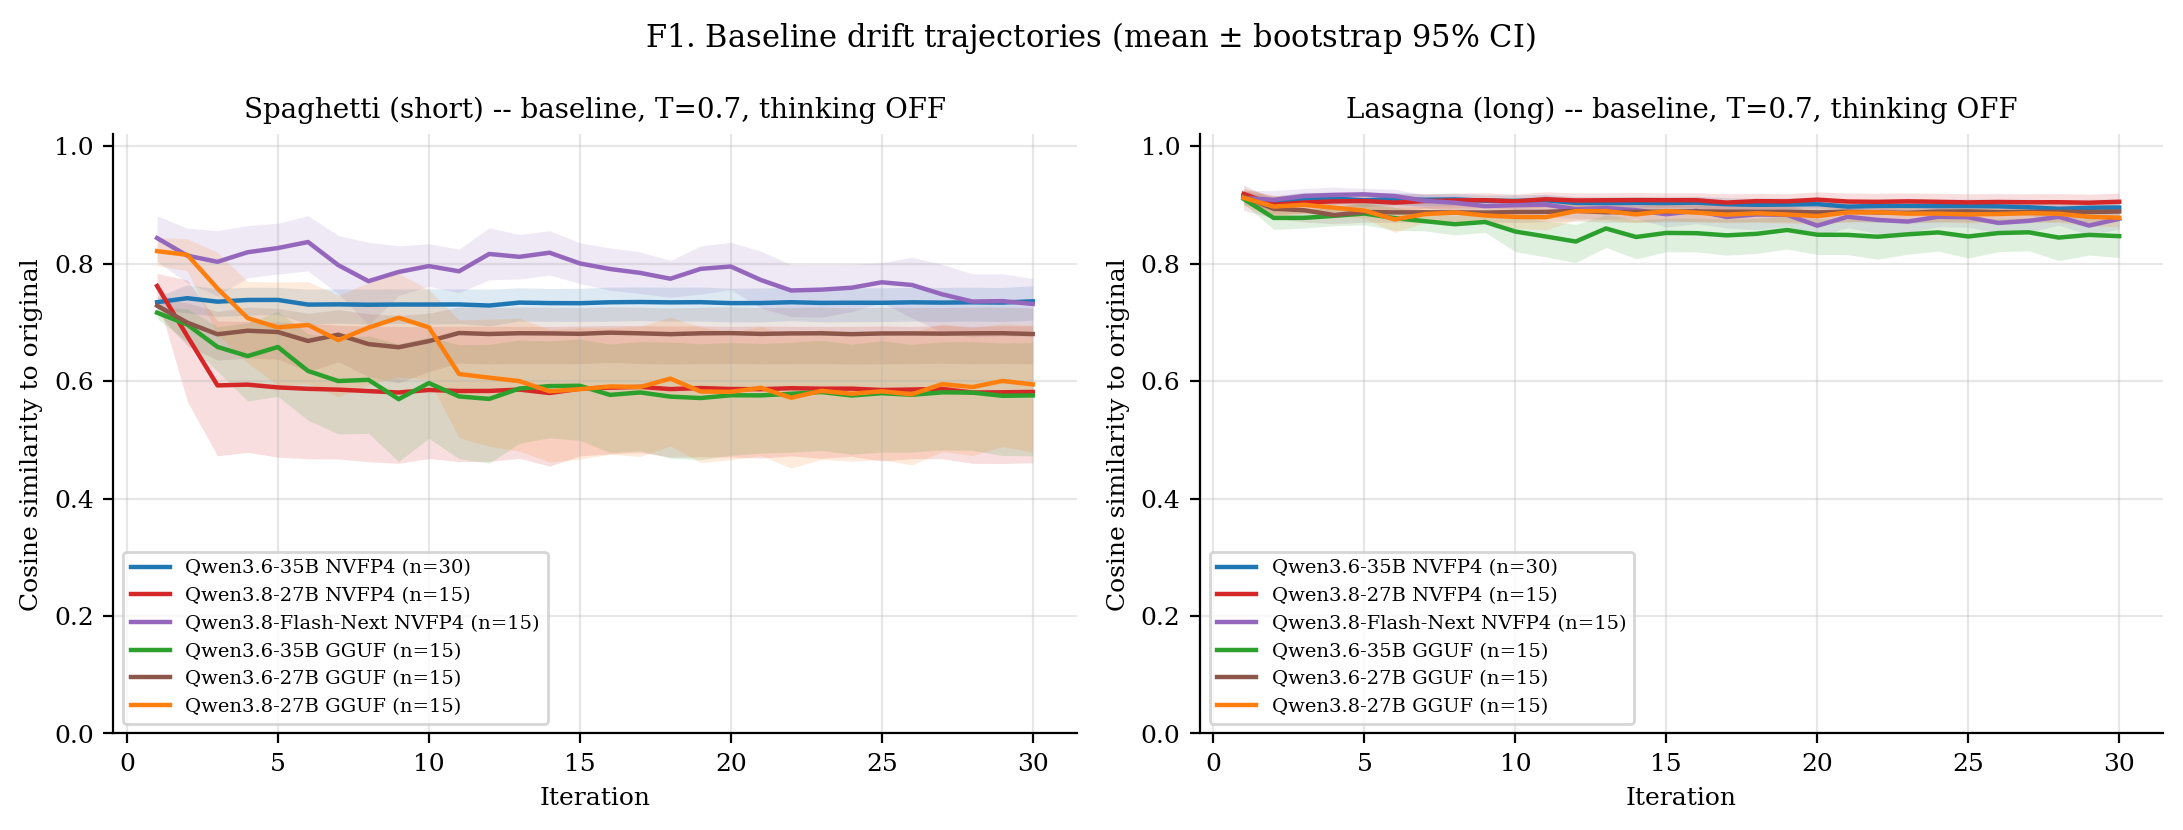
\includegraphics[width=\textwidth,height=0.33\textheight,keepaspectratio]{../results/paper3_figures/fig1_baseline_trajectories.png}
\caption{Baseline drift trajectories for the six non-MTP configurations,
  mean with bootstrap band; $n$ in the legend. Left: spaghetti. Right:
  lasagna.}
\label{fig:baseline}
\end{figure}

\begin{table}[t]
\centering
\caption{Baseline drift at iteration 30 (T=0.7, no system prompt, thinking OFF).
Means over independent chains with percentile bootstrap 95\% CIs ($B$=10{,}000).
Locked = last three outputs byte-identical; inflation = final output words divided
by prompt words; meta = final output contains agent-handoff / meta-commentary
markers. The two Qwen3.6-35B NVFP4 hosts are pooled.}
\label{tab:paper3-baseline}
\resizebox{\textwidth}{!}{%
\begin{tabular}{llrlrrrr}
\toprule
Configuration & Recipe & Mean & 95\% CI & $n$ & Locked & Inflation & Meta \\
\midrule
Qwen3.6-35B NVFP4 & Spaghetti & 0.736 & [0.703, 0.763] & 30 & 0.87 & 5.64 & 1.00 \\
Qwen3.6-35B NVFP4 & Lasagna & 0.896 & [0.878, 0.910] & 30 & 0.87 & 1.02 & 0.83 \\
Qwen3.8-27B NVFP4 & Spaghetti & 0.582 & [0.458, 0.690] & 15 & 0.93 & 7.21 & 1.00 \\
Qwen3.8-27B NVFP4 & Lasagna & 0.905 & [0.891, 0.919] & 15 & 0.93 & 1.05 & 0.87 \\
Qwen3.8-Flash-Next NVFP4 & Spaghetti & 0.731 & [0.675, 0.777] & 15 & 0.20 & 5.71 & 0.80 \\
Qwen3.8-Flash-Next NVFP4 & Lasagna & 0.876 & [0.859, 0.892] & 15 & 0.00 & 1.03 & 0.60 \\
Qwen3.6-35B GGUF & Spaghetti & 0.576 & [0.472, 0.668] & 15 & 0.73 & 6.83 & 1.00 \\
Qwen3.6-35B GGUF & Lasagna & 0.847 & [0.810, 0.876] & 15 & 0.93 & 0.96 & 0.80 \\
Qwen3.6-27B GGUF & Spaghetti & 0.680 & [0.629, 0.726] & 15 & 0.93 & 7.19 & 1.00 \\
Qwen3.6-27B GGUF & Lasagna & 0.889 & [0.873, 0.905] & 15 & 1.00 & 1.01 & 0.87 \\
Qwen3.8-27B GGUF & Spaghetti & 0.594 & [0.481, 0.695] & 15 & 0.60 & 6.17 & 0.93 \\
Qwen3.8-27B GGUF & Lasagna & 0.878 & [0.863, 0.891] & 15 & 0.87 & 1.10 & 1.00 \\
Qwen3.8-27B GGUF+MTP & Spaghetti & 0.532 & [0.411, 0.648] & 15 & 0.73 & 6.85 & 0.93 \\
Qwen3.8-27B GGUF+MTP & Lasagna & 0.897 & [0.885, 0.909] & 15 & 0.80 & 1.07 & 0.87 \\
\bottomrule
\end{tabular}}
\end{table}


\paragraph{Across generations.}
Figure~\ref{fig:crossgen} and Table~\ref{tab:paper3-crossgen} place these
results beside Paper~A's Qwen3 pilot and Qwen3.5 data at matched size,
using Paper~A's clean chains (those without runaway failures) for the
Qwen3.5 rows. On the short stimulus the trend is monotonically downward
after Qwen3.5: the 27B dense line runs 0.564 (Qwen3-32B, single pilot
chain), 0.914 (Qwen3.5), 0.680 (Qwen3.6), 0.594 (Qwen3.8), and the
35B-class MoE line 0.806, 0.923, 0.576 (GGUF) or 0.736 (NVFP4); the 122B
class falls from 0.925 (Qwen3.5-122B) to 0.731 (Flash-Next). On the long
stimulus the newer generations are as good or better: 0.829 (Qwen3.5-27B)
against 0.889 and 0.878--0.905, and 0.812--0.845 against 0.847--0.896 for the
35B class. The Qwen3.5 short-stimulus values rest on two to three clean
chains each and are existence results, as Paper~A notes; the newer values
rest on fifteen to thirty. The pattern is nonetheless consistent with
everything else in this paper: the newer models paraphrase a long document
faithfully and cannot leave a short one alone.

\begin{figure}[htbp]
\centering
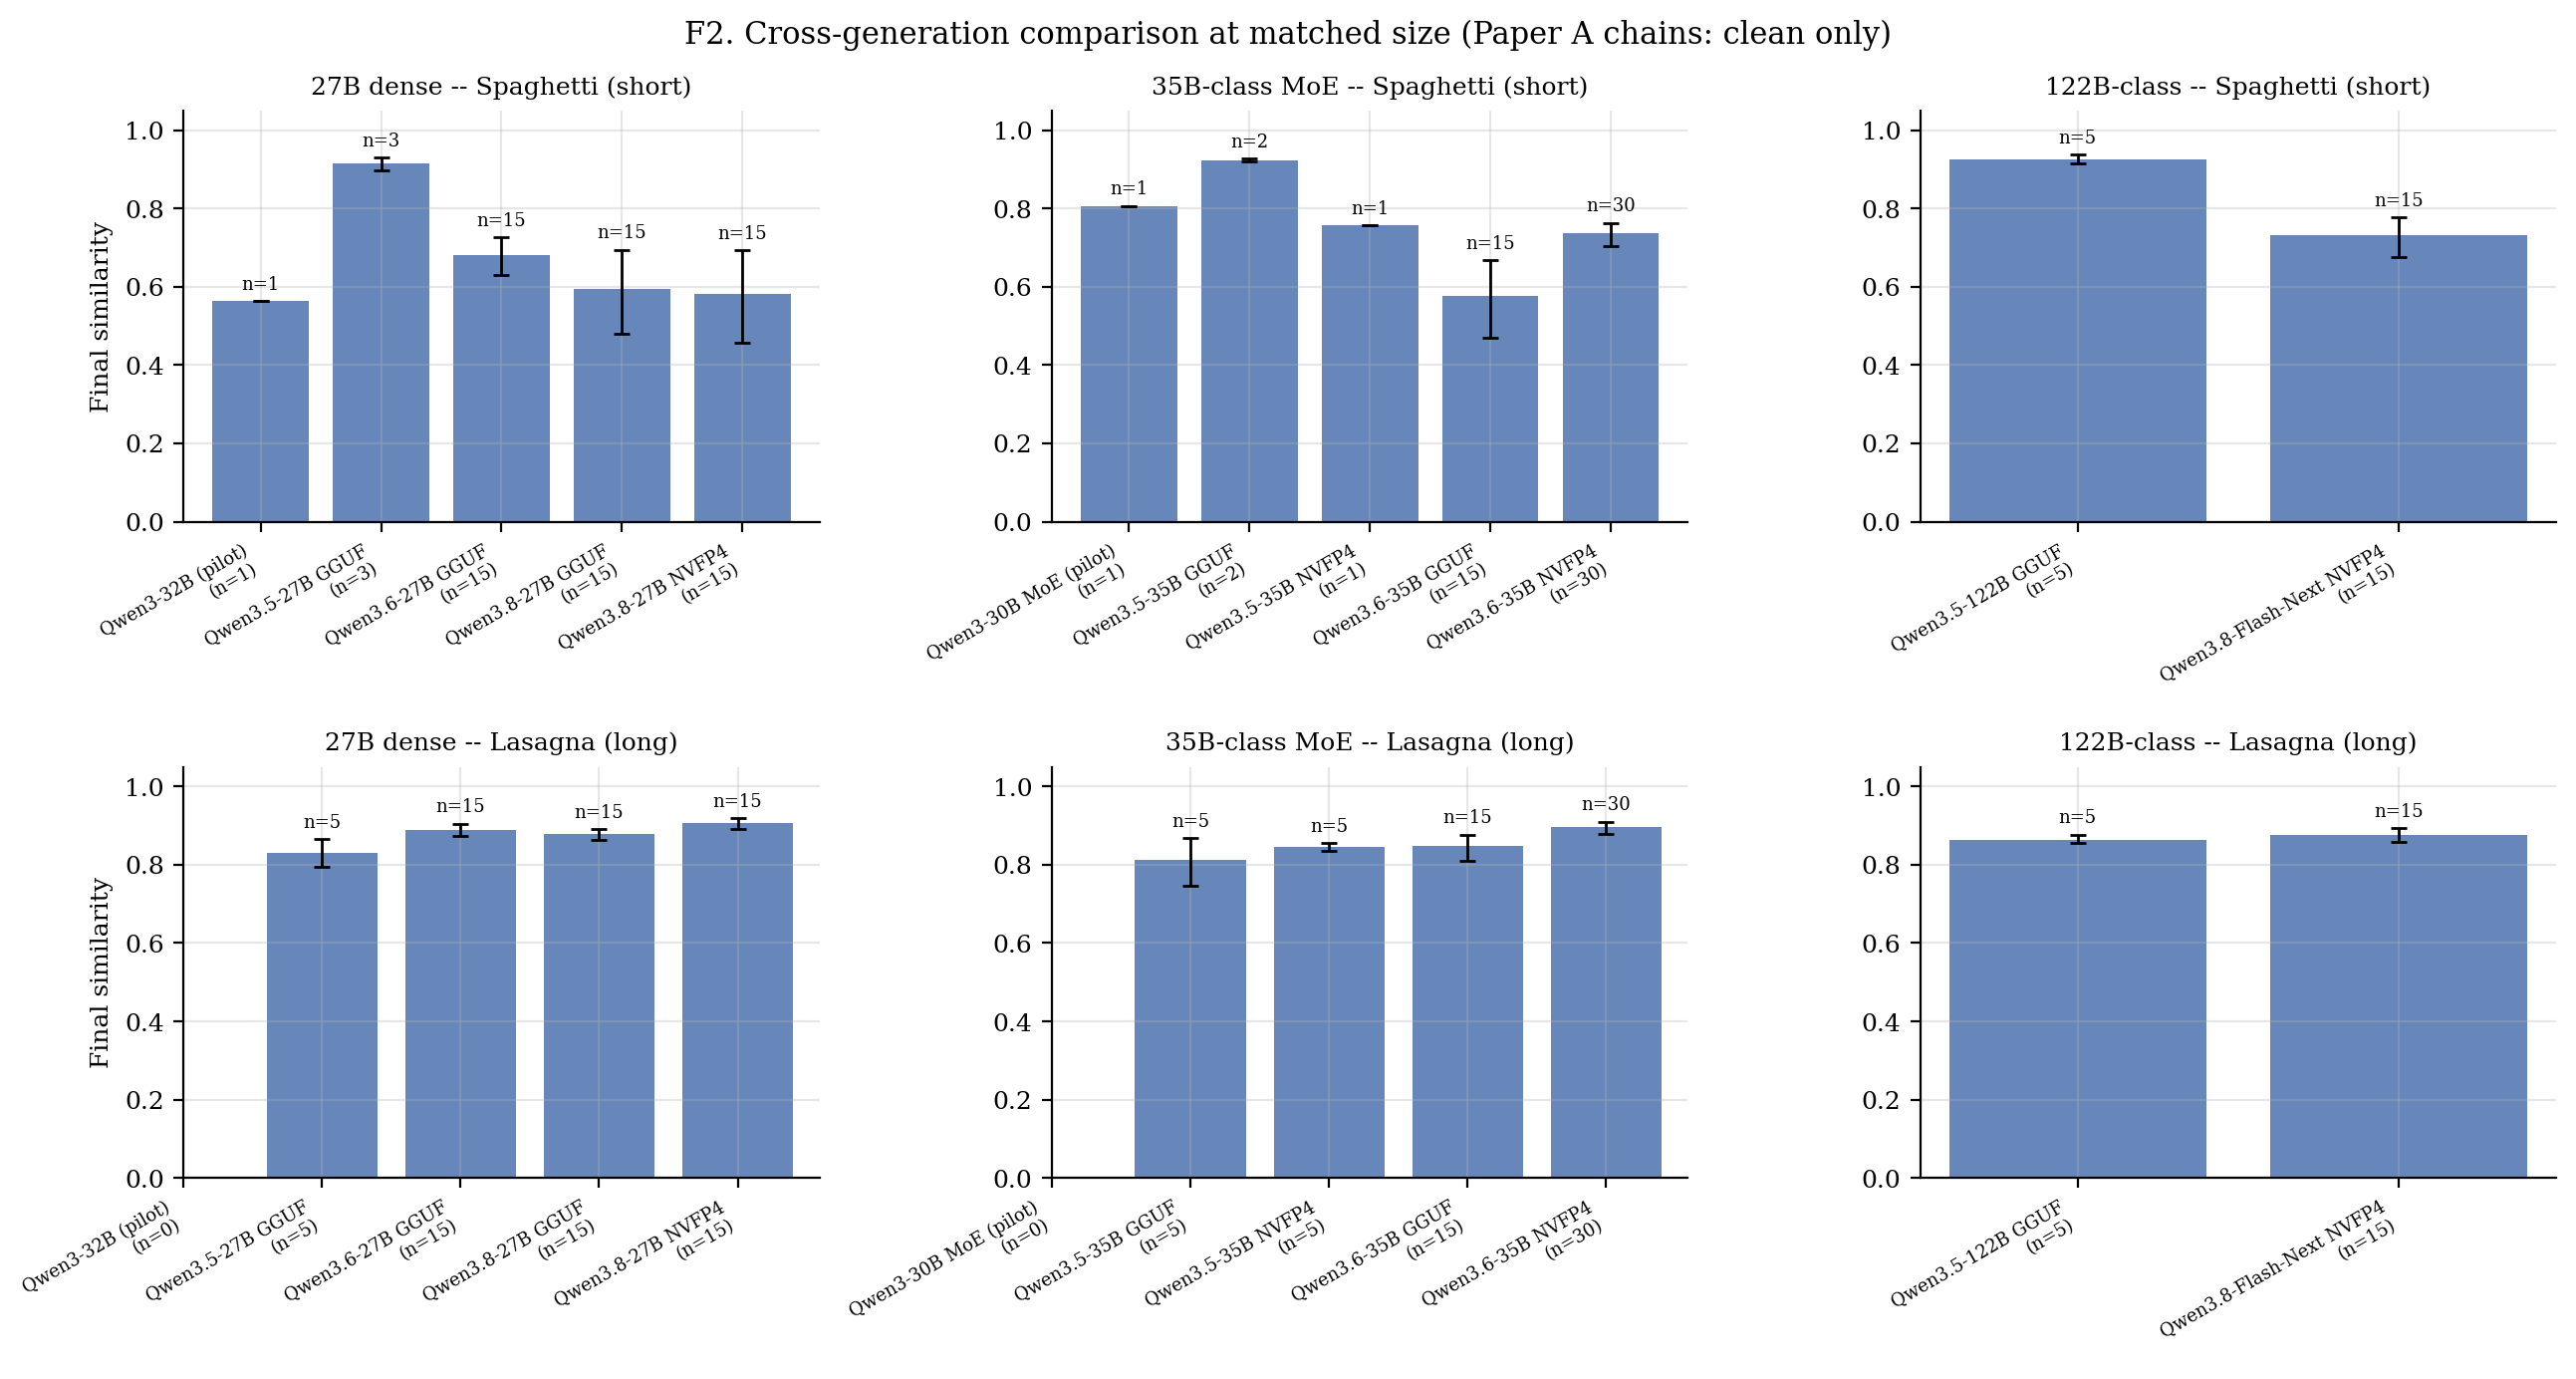
\includegraphics[width=\textwidth,height=0.33\textheight,keepaspectratio]{../results/paper3_figures/fig2_cross_generation.png}
\caption{Final similarity at matched model size across four Qwen
  generations. Qwen3 values are single unseeded pilot chains and have no
  lasagna run; Qwen3.5 values are Paper~A's clean chains only, with $n$
  shown. Error bars are bootstrap 95\% intervals.}
\label{fig:crossgen}
\end{figure}

\begin{table}[t]
\centering
\caption{Cross-generation drift at matched model size. Paper~A rows use clean chains
only (no empty output in any successful iteration); the Qwen3 pilot is a single
unseeded chain per model. Bootstrap 95\% CIs, $B$=10{,}000.}
\label{tab:paper3-crossgen}
\resizebox{\textwidth}{!}{%
\begin{tabular}{lrlrrl}
\toprule
Model & \multicolumn{3}{c}{Spaghetti} & \multicolumn{2}{c}{Lasagna} \\
\cmidrule(lr){2-4}\cmidrule(lr){5-6}
 & Mean & 95\% CI & $n$ & Mean & 95\% CI \\
\midrule
\multicolumn{6}{l}{\textit{27B dense}} \\
\quad Qwen3-32B (pilot) & 0.564 & [0.564, 0.564] & 1 & --- & --- \\
\quad Qwen3.5-27B GGUF & 0.914 & [0.898, 0.929] & 3 & 0.829 & [0.793, 0.866] \\
\quad Qwen3.6-27B GGUF & 0.680 & [0.630, 0.727] & 15 & 0.889 & [0.872, 0.905] \\
\quad Qwen3.8-27B GGUF & 0.594 & [0.480, 0.694] & 15 & 0.878 & [0.864, 0.891] \\
\quad Qwen3.8-27B NVFP4 & 0.582 & [0.456, 0.693] & 15 & 0.905 & [0.891, 0.919] \\
\addlinespace
\multicolumn{6}{l}{\textit{35B-class MoE}} \\
\quad Qwen3-30B MoE (pilot) & 0.806 & [0.806, 0.806] & 1 & --- & --- \\
\quad Qwen3.5-35B GGUF & 0.923 & [0.920, 0.927] & 2 & 0.812 & [0.746, 0.867] \\
\quad Qwen3.5-35B NVFP4 & 0.757 & [0.757, 0.757] & 1 & 0.845 & [0.836, 0.854] \\
\quad Qwen3.6-35B GGUF & 0.576 & [0.470, 0.667] & 15 & 0.847 & [0.811, 0.876] \\
\quad Qwen3.6-35B NVFP4 & 0.736 & [0.703, 0.763] & 30 & 0.896 & [0.878, 0.910] \\
\addlinespace
\multicolumn{6}{l}{\textit{122B-class}} \\
\quad Qwen3.5-122B GGUF & 0.925 & [0.915, 0.937] & 5 & 0.864 & [0.856, 0.877] \\
\quad Qwen3.8-Flash-Next NVFP4 & 0.731 & [0.675, 0.777] & 15 & 0.876 & [0.859, 0.892] \\
\addlinespace
\bottomrule
\end{tabular}}
\end{table}


\subsection{Seeds do not reproduce chains}
\label{sec:seeds}

Every experiment in Paper~A, and in the prior literature we are aware of,
labels repeated runs by sampling seed on the assumption that the seed fixes
the trajectory. Figure~\ref{fig:determinism} and
Table~\ref{tab:paper3-determinism} test that assumption on host A. Ten
seeds run twice produced ten pairs of chains that differed at iteration~1 in
every case, with zero identical iterations in any pair and final
similarities differing by 0.045 on average (maximum 0.096). Running the same
five seeds twice with a single request in flight, so that no other request
could share a batch, changed nothing: all five pairs diverged at
iteration~1. Two byte-identical single requests at temperature~0 with the
same seed returned different text, disagreeing at about the ninth token. The
deployment---an NVFP4 mixture-of-experts on a FlashInfer backend with prefix
caching---is not batch-invariant in the sense of
\citet{he2025nondeterminism}, and neither the seed nor greedy decoding
restores reproducibility.

What does replicate is the distribution. Host A and host B, two identical
deployments on different machines, give baseline means that are
statistically indistinguishable (spaghetti 0.749 vs.\ 0.723, $p=0.63$;
lasagna 0.904 vs.\ 0.887, $p=0.38$), and every ranking reported later in
this paper agrees across the two hosts at $\rho\geq0.95$. Temperature~0
does narrow the spread: at 15 samples per condition the standard deviation
of final similarity falls from 0.089 to 0.016 on Qwen3.6-35B spaghetti and
from 0.240 to 0.070 on Qwen3.8-27B spaghetti, but the means move by less
than 0.05 in five of six cases (the exception is Flash-Next on lasagna,
0.918 against 0.876, $p<0.001$). Greedy decoding is a variance reduction,
not a fidelity improvement, and it is not reproducible either.

The consequence for method is that a ``seed'' is one draw from the model's
output distribution under that deployment. We therefore report every
condition as a sample of 15 to 30 chains with a bootstrap interval, we never
pair chains by seed, and we regard the roughly 0.05 within-host difference
between draws as the noise floor below which a contrast between conditions
is not interpretable.

\begin{figure}[htbp]
\centering
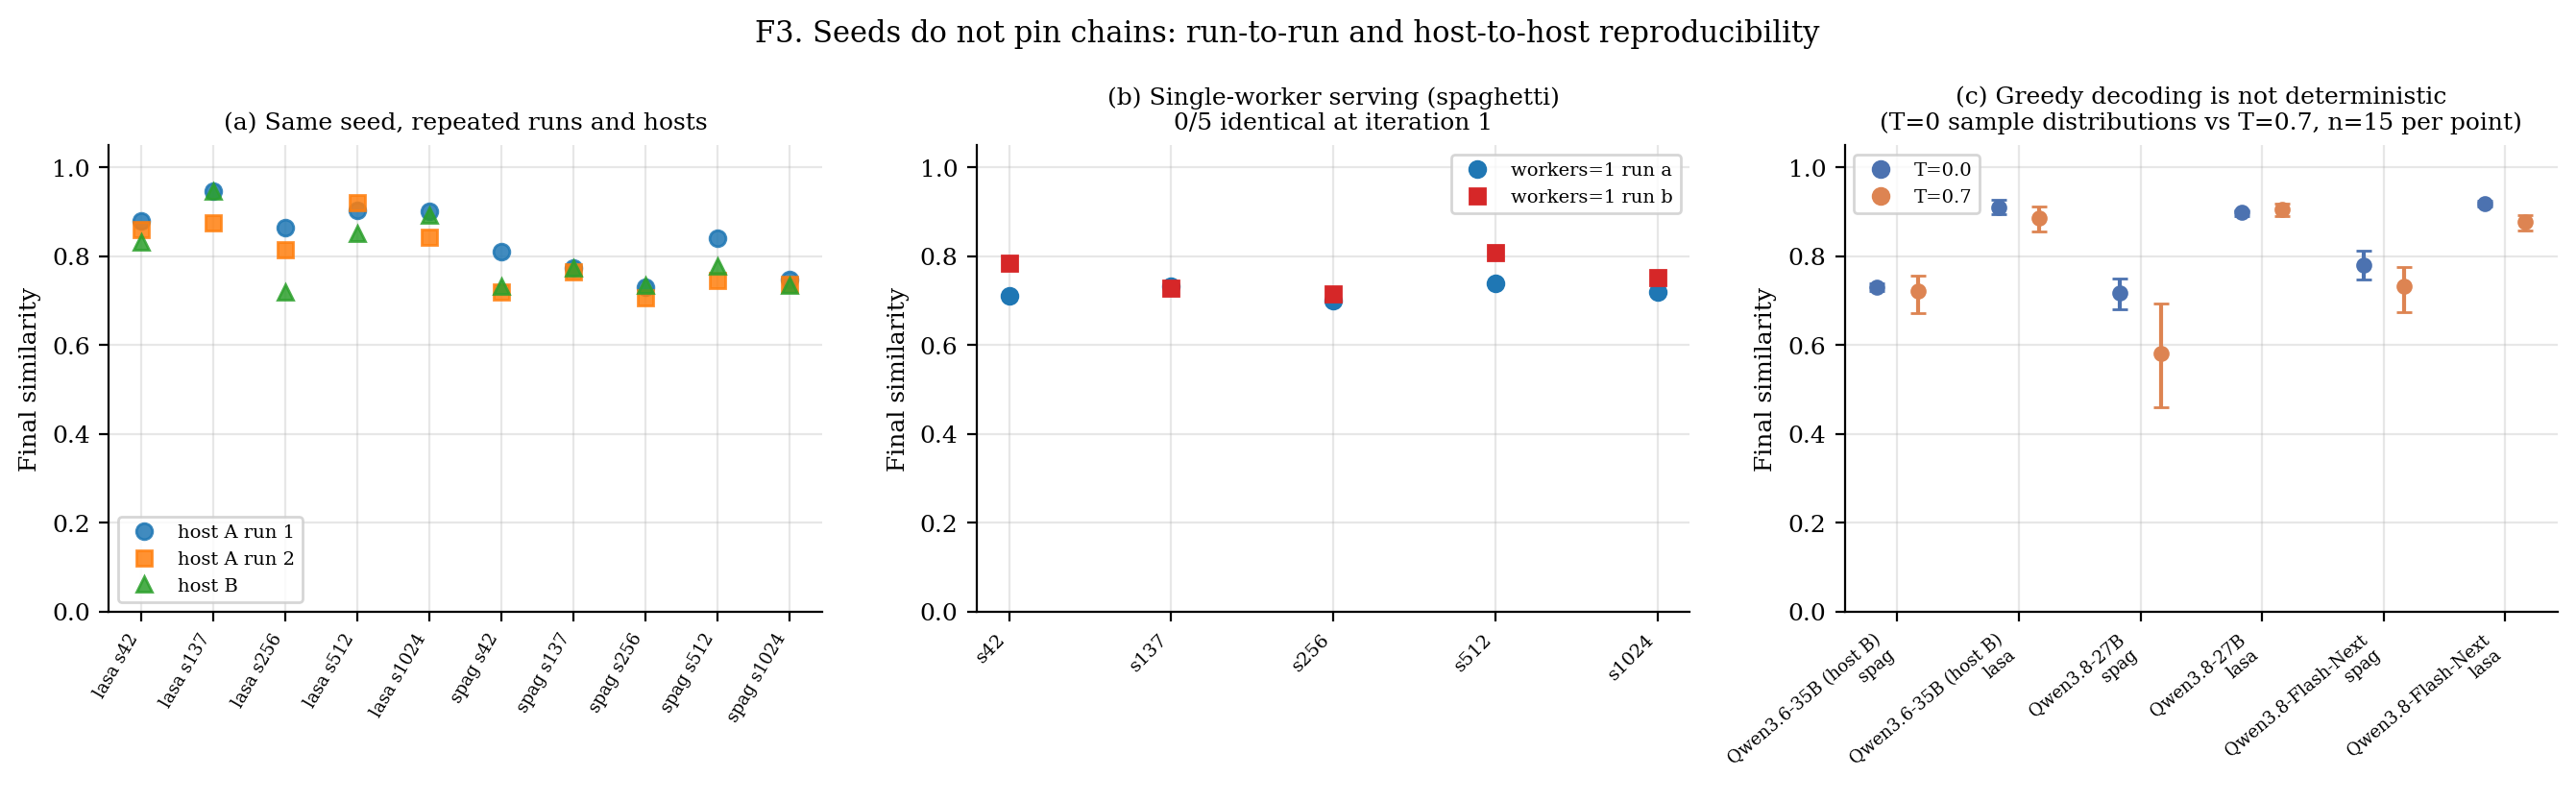
\includegraphics[width=\textwidth,height=0.33\textheight,keepaspectratio]{../results/paper3_figures/fig3_determinism.png}
\caption{Seed reproducibility. (a) Final similarity for ten seeds run twice
  on host A and once on host B. (b) The same for five seeds with a single
  request in flight. (c) Distributions of final similarity at $T=0$ and
  $T=0.7$, 15 samples each, three models.}
\label{fig:determinism}
\end{figure}

\begin{table}[t]
\centering
\caption{Seed reproducibility. Chains repeated with identical seed, prompt and
deployment diverge immediately; ``identical at iter.\ 1'' counts pairs whose first
outputs are byte-identical, and $|\Delta|$ is the absolute difference in final
similarity. The lower block compares the two Qwen3.6-35B NVFP4 hosts as
distributions (Mann--Whitney U, $n$=15 per host per recipe).}
\label{tab:paper3-determinism}
\resizebox{\textwidth}{!}{%
\begin{tabular}{lrrrrr}
\toprule
Comparison & pairs & identical at iter.\ 1 & mean identical iters & mean $|\Delta|$ & max $|\Delta|$ \\
\midrule
host A run1 vs run2 & 10 & 0/10 & 0.00 & 0.045 & 0.096 \\
host A run1 vs host B & 10 & 1/10 & 3.00 & 0.041 & 0.144 \\
host A workers=1 run a vs run b & 5 & 0/5 & 0.00 & 0.040 & 0.074 \\
\bottomrule
\end{tabular}}

\vspace{1em}
\resizebox{\textwidth}{!}{%
\begin{tabular}{lrrr}
\toprule
Recipe & host A mean ($n$) & host B mean ($n$) & MWU $p$ \\
\midrule
spaghetti & 0.749 (15) & 0.723 (15) & 0.6333 \\
lasagna & 0.904 (15) & 0.887 (15) & 0.3837 \\
\bottomrule
\end{tabular}}
\end{table}


\subsection{Thinking mode}
\label{sec:thinking}

Table~\ref{tab:paper3-thinking} and Figure~\ref{fig:thinking} give the
central result of this section: enabling reasoning changes drift by 0.03 to
0.30 in every condition, significant in all eight, and the direction is a
property of the model. Qwen3.6-35B loses 0.09 on spaghetti and 0.15--0.16 on
lasagna, identically on both hosts, while generating 1{,}400--3{,}100
reasoning tokens per iteration. Qwen3.8-27B gains 0.30 on spaghetti and
0.03 on lasagna with only 110--440 reasoning tokens, and Flash-Next gains
0.14 and 0.06 with 95--310. Thinking also collapses the variance of the
model it helps: Qwen3.8-27B's spaghetti standard deviation falls from 0.24
to 0.02, because the reasoning step suppresses the failure that dominates
its baseline, in which the model answers the paraphrase request with a menu
of three options, the next iteration paraphrases the menu, and the chain
locks into a memo about a missing source text at similarity 0.14.

\begin{figure}[htbp]
\centering
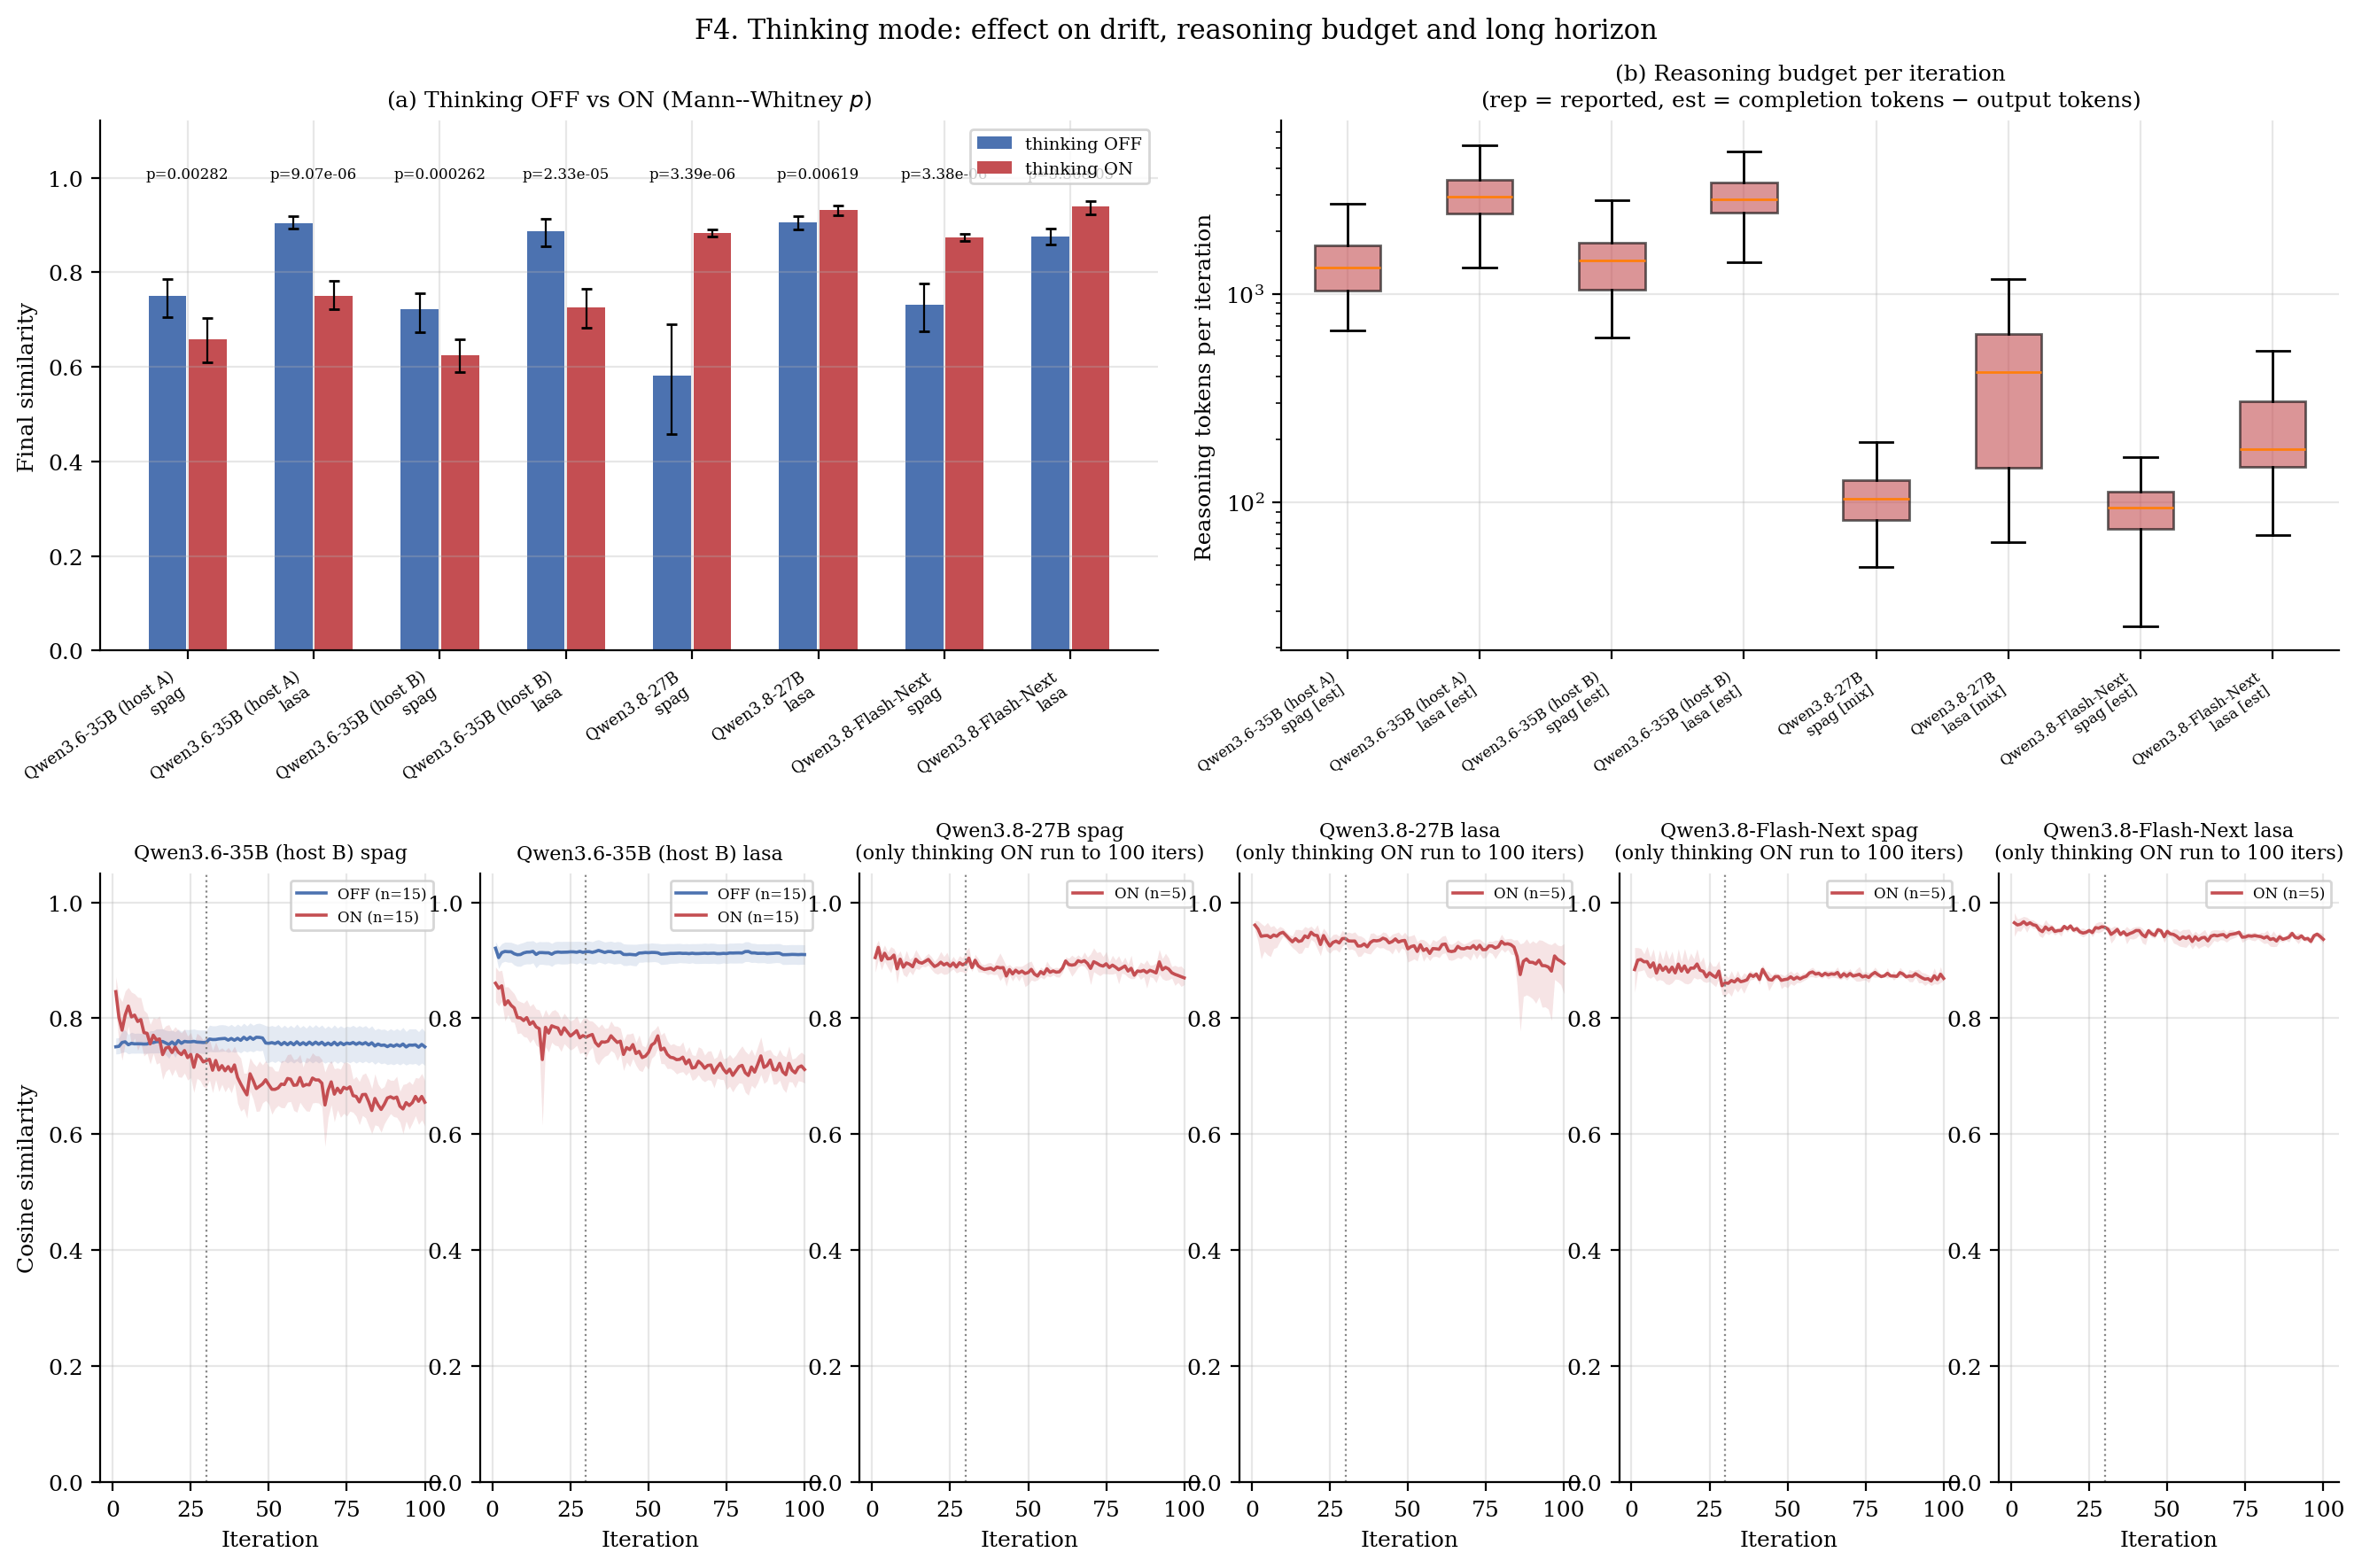
\includegraphics[width=\textwidth,height=0.4\textheight,keepaspectratio]{../results/paper3_figures/fig4_thinking.png}
\caption{Thinking mode. (a) Final similarity with thinking off and on, per
  configuration and recipe. (b) Reasoning tokens per iteration. (c)
  100-iteration trajectories with thinking off and on.}
\label{fig:thinking}
\end{figure}

\begin{table}[t]
\centering
\caption{Thinking mode. Upper block: final similarity with thinking OFF and ON
(mean with $n$ chains), the ON$-$OFF difference, Mann--Whitney $p$, and the mean
reasoning tokens per iteration. ``rep'' = reasoning token counts reported by the
server; ``est'' = completion tokens minus output tokens (4 characters per token).
Lower block: 100-iteration runs, similarity at iteration 30 and 100 and the fraction
of chains dipping more than 0.05 below their iteration-30 value.}
\label{tab:paper3-thinking}
\resizebox{\textwidth}{!}{%
\begin{tabular}{llrrrrrl}
\toprule
Configuration & Recipe & OFF ($n$) & ON ($n$) & $\Delta$ & $p$ & Reas.\ tok/iter & Source \\
\midrule
Qwen3.6-35B NVFP4 (host A) & spaghetti & 0.749 (15) & 0.658 (15) & -0.091 & 0.0028 & 1420 & estimated \\
Qwen3.6-35B NVFP4 (host A) & lasagna & 0.904 (15) & 0.750 (15) & -0.154 & $<$0.0001 & 3095 & estimated \\
Qwen3.6-35B NVFP4 (host B) & spaghetti & 0.723 (15) & 0.625 (15) & -0.097 & 0.0003 & 1466 & estimated \\
Qwen3.6-35B NVFP4 (host B) & lasagna & 0.887 (15) & 0.726 (15) & -0.160 & $<$0.0001 & 2975 & estimated \\
Qwen3.8-27B NVFP4 & spaghetti & 0.582 (15) & 0.883 (15) & 0.302 & $<$0.0001 & 110 & estimated/reported \\
Qwen3.8-27B NVFP4 & lasagna & 0.905 (15) & 0.932 (15) & 0.026 & 0.0062 & 436 & estimated/reported \\
Qwen3.8-Flash-Next NVFP4 & spaghetti & 0.731 (15) & 0.873 (15) & 0.141 & $<$0.0001 & 95 & estimated \\
Qwen3.8-Flash-Next NVFP4 & lasagna & 0.876 (15) & 0.939 (15) & 0.063 & $<$0.0001 & 306 & estimated \\
\bottomrule
\end{tabular}}

\vspace{1em}
\resizebox{\textwidth}{!}{%
\begin{tabular}{lllrrrrr}
\toprule
Configuration & Recipe & Think & $n$ & @30 & @100 & $\Delta_{30\to100}$ & dip rate \\
\midrule
Qwen3.6-35B NVFP4 (host B) & spaghetti & OFF & 15 & 0.759 & 0.751 & -0.008 & 0.07 \\
Qwen3.6-35B NVFP4 (host B) & spaghetti & ON & 15 & 0.727 & 0.655 & -0.072 & 0.73 \\
Qwen3.6-35B NVFP4 (host B) & lasagna & OFF & 15 & 0.915 & 0.910 & -0.005 & 0.13 \\
Qwen3.6-35B NVFP4 (host B) & lasagna & ON & 15 & 0.767 & 0.712 & -0.056 & 1.00 \\
Qwen3.8-27B NVFP4 & spaghetti & ON & 5 & 0.895 & 0.870 & -0.025 & 0.40 \\
Qwen3.8-27B NVFP4 & lasagna & ON & 5 & 0.938 & 0.894 & -0.043 & 0.60 \\
Qwen3.8-Flash-Next NVFP4 & spaghetti & ON & 5 & 0.861 & 0.869 & 0.008 & 0.00 \\
Qwen3.8-Flash-Next NVFP4 & lasagna & ON & 5 & 0.957 & 0.936 & -0.021 & 0.20 \\
\bottomrule
\end{tabular}}
\end{table}


\paragraph{No fixed point.}
With thinking off, 100-iteration chains on host B are flat after
iteration~30: the mean moves by $-0.008$ (spaghetti) and $-0.005$ (lasagna)
between iterations 30 and 100, and only one to two of fifteen chains dip by
more than 0.05 in that span. With thinking on the same model keeps
drifting: $-0.072$ and $-0.056$ over the same span, with 73\% and 100\% of
chains dipping, reaching 0.56 and 0.63 at their minima. Qwen3.8-27B with
thinking drifts mildly over 100 iterations and Flash-Next holds. A
reasoning model that rewrites a text is, on this evidence, not an iterated
function with a fixed point; each pass reconsiders the document.

\paragraph{No prompt rescues it.}
On Qwen3.6-35B lasagna with all 20 system prompts, thinking on is worse
than thinking off for 18 of the 20 (mean $-0.053$), the best prompt with
thinking (Precise Transmitter, 0.915) merely matches the no-prompt baseline
without thinking (0.913), and the prompt ranking with thinking correlates
only weakly with the ranking without ($\rho=0.43$). Where thinking helps,
in Qwen3.8-27B, it does so because a short reasoning pass suppresses a
formatting failure; where it hurts, the reasoning pass rewrites the
document from its own summary of it, and the prompt cannot reach that
summary.

\paragraph{Runaway thinking persists at a low rate.}
Paper~A found that Qwen3.5 with reasoning enabled exhausted its 16{,}384-
token budget inside the thinking block in 13.5\% of chains. Here every one
of the 2{,}222 thinking-off chains produced text at every iteration
(runaway rate 0, Wilson interval $[0, 0.17\%]$), and so did every
thinking-on chain on Qwen3.8-27B and Flash-Next. On Qwen3.6-35B with
thinking on, 17 of the 300 such chains (5.7\%) contained at least one
iteration that hit the budget, concentrated in the lasagna system-prompt conditions and
the long construction document, and 13 of those returned an empty
completion. The failure Paper~A described has therefore been reduced by an
order of magnitude in the following generation and removed in the one after,
but it has not disappeared, and the prompts that trigger it (Visual
Tutorial Style, Friendly Conversational, Multimodal Visual Focus) are the
verbose ones rather than, as in Qwen3.5, the constraining ones.

\paragraph{The sampler controls it.}
Paper~A could not separate the serving stack from the sampling defaults each
stack applies, because its requests set only temperature and seed. We
therefore took the worst condition above---Visual Tutorial Style on
lasagna, where the server default sampler hit the token cap in 8 of 15
chains---and reran it under two explicit samplers. With top-$k$ and top-$p$
removed (a bare sampler) the cap was hit in 5 of 15 chains, not
distinguishable from the default ($p=0.46$, Fisher). With the vendor's
recommended thinking-mode sampler, which adds a presence penalty of 1.5, the
cap was hit in 0 of 15 chains ($p=0.002$ against the default, $p=0.04$
against the bare sampler), the longest single reply fell from the 16{,}384
cap to 14{,}225 tokens, and mean reply length fell by 8\%. Final similarity
was unchanged (0.56, 0.58, 0.59; $p=0.74$). The bare sampler on plain
spaghetti, where the default rate is zero, stayed at zero. Runaway thinking
is therefore not a property of a serving stack but of sampling the reasoning
block without a repetition control, which is exactly the setting the Qwen
model cards warn against; a presence penalty removes the failure without
changing what the model produces when it does answer. This also resolves
the stack ordering Paper~A reported: the Ollama library's Qwen3.5 tags ship
a parameter layer with exactly this sampler (top-$k$ 20, top-$p$ 0.95,
presence penalty 1.5), so Paper~A's Ollama arm ran penalised and its SGLang
arm did not, and the Ollama arm's lower but non-zero rate (15--27\% against
36--54\%) shows that on Qwen3.5 the penalty mitigates the failure where on
Qwen3.6 it removes it.

\subsection{Serving format, stack, and speculative decoding}
\label{sec:format}

Paper~A found that 4-bit builds of the same Qwen3.5 weights differed by up
to 0.26 on the short stimulus depending on format and serving stack.
Table~\ref{tab:paper3-format} and Figure~\ref{fig:format} repeat the
comparison on two new generations, with the caveat that the GGUF arm here
differs from the NVFP4 arm in quantization, serving software, KV-cache
precision and GPU generation at once (Appendix~\ref{app:compute}). For
Qwen3.6-35B the NVFP4 build on vLLM is better on both recipes (0.736 vs.\
0.576 on spaghetti, $p<0.001$; 0.896 vs.\ 0.847 on lasagna, $p=0.006$). For
Qwen3.8-27B the two builds are indistinguishable on spaghetti (0.582 vs.\
0.594, $p=0.93$) and the NVFP4 build is slightly better on lasagna (0.905
vs.\ 0.878, $p=0.016$). The direction of Paper~A's effect, which favoured
GGUF, is not reproduced; its magnitude on one of the two models is.

\begin{figure}[htbp]
\centering
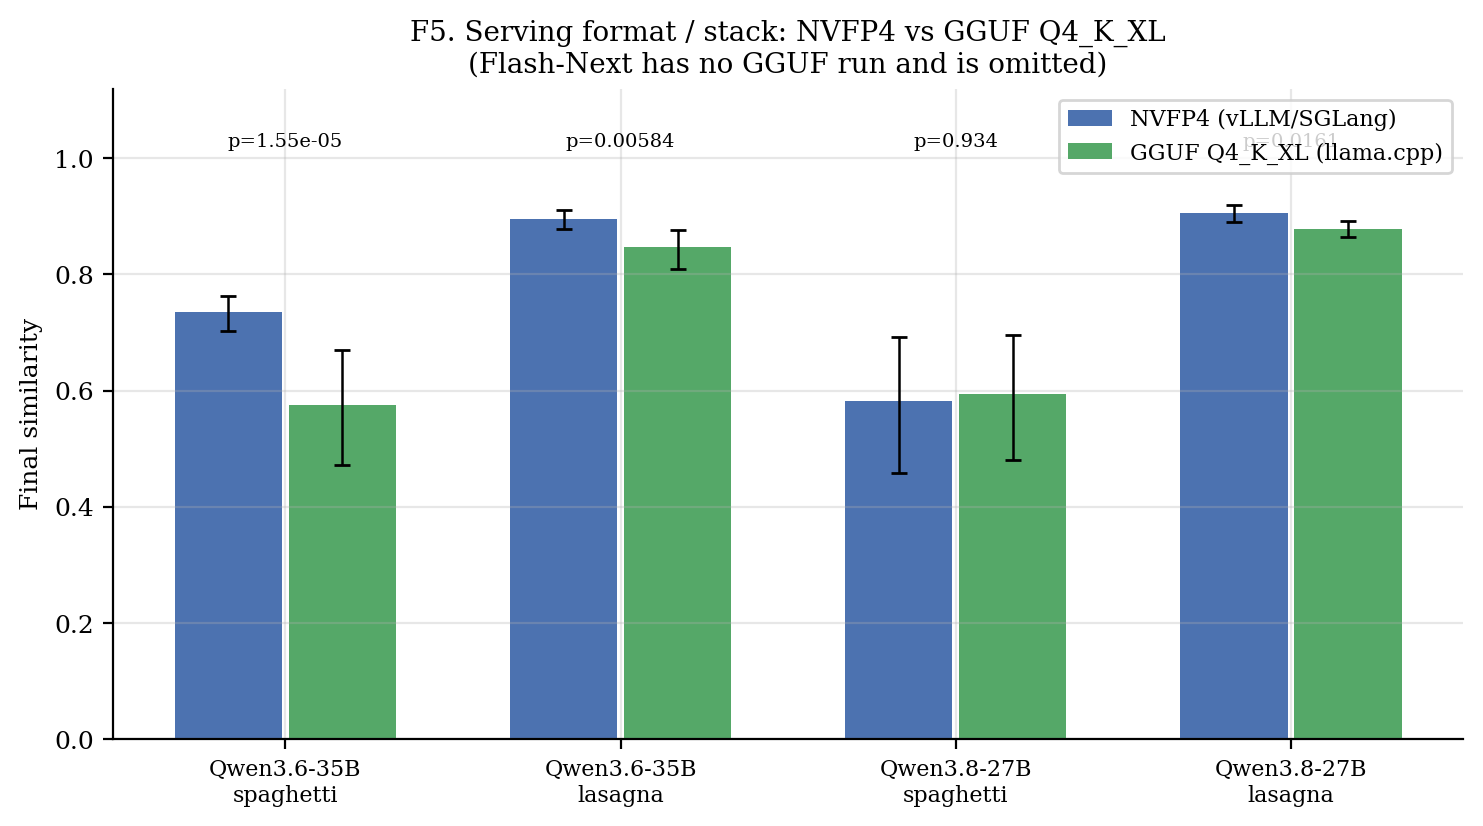
\includegraphics[width=0.85\textwidth,height=0.3\textheight,keepaspectratio]{../results/paper3_figures/fig5_format_stack.png}
\caption{NVFP4 on vLLM against GGUF Q4\_K\_XL on llama.cpp for the same
  weights, both recipes, with bootstrap intervals.}
\label{fig:format}
\end{figure}

\begin{table}[t]
\centering
\caption{Serving format and stack. Same weights family, two quantisation formats and
two inference stacks (NVFP4 on vLLM/SGLang vs GGUF Q4\_K\_XL on llama.cpp).
Qwen3.8-Flash-Next has no GGUF run and is omitted.}
\label{tab:paper3-format}
\resizebox{\textwidth}{!}{%
\begin{tabular}{llrrrrrr}
\toprule
Model & Recipe & NVFP4 mean [CI] & $n$ & GGUF mean [CI] & $n$ & $\Delta$ & MWU $p$ \\
\midrule
Qwen3.6-35B & spaghetti & 0.736 [0.703, 0.763] & 30 & 0.576 [0.471, 0.670] & 15 & 0.160 & $<$0.0001 \\
Qwen3.6-35B & lasagna & 0.896 [0.878, 0.911] & 30 & 0.847 [0.810, 0.876] & 15 & 0.049 & 0.0058 \\
Qwen3.8-27B & spaghetti & 0.582 [0.457, 0.693] & 15 & 0.594 [0.481, 0.696] & 15 & -0.013 & 0.9339 \\
Qwen3.8-27B & lasagna & 0.905 [0.891, 0.919] & 15 & 0.878 [0.864, 0.892] & 15 & 0.027 & 0.0161 \\
\bottomrule
\end{tabular}}
\end{table}


\paragraph{Speculative decoding is a null.}
The Qwen3.8-27B GGUF file served with and without its multi-token-prediction
draft head is the cleanest infrastructure comparison in either paper: same
bytes, same server, one flag. Figure~\ref{fig:mtp} shows no difference
(spaghetti 0.594 vs.\ 0.532, $p=0.44$; lasagna 0.878 vs.\ 0.897, $p=0.12$;
15 samples each). Draft-and-verify sampling is distribution-preserving in
theory~\citep{leviathan2023speculative,chen2023speculative}, and for drift
it is so in practice. An earlier five-sample reading of the same comparison
had suggested a large penalty; it did not survive replication, which is the
point of Section~\ref{sec:seeds}.

\begin{figure}[htbp]
\centering
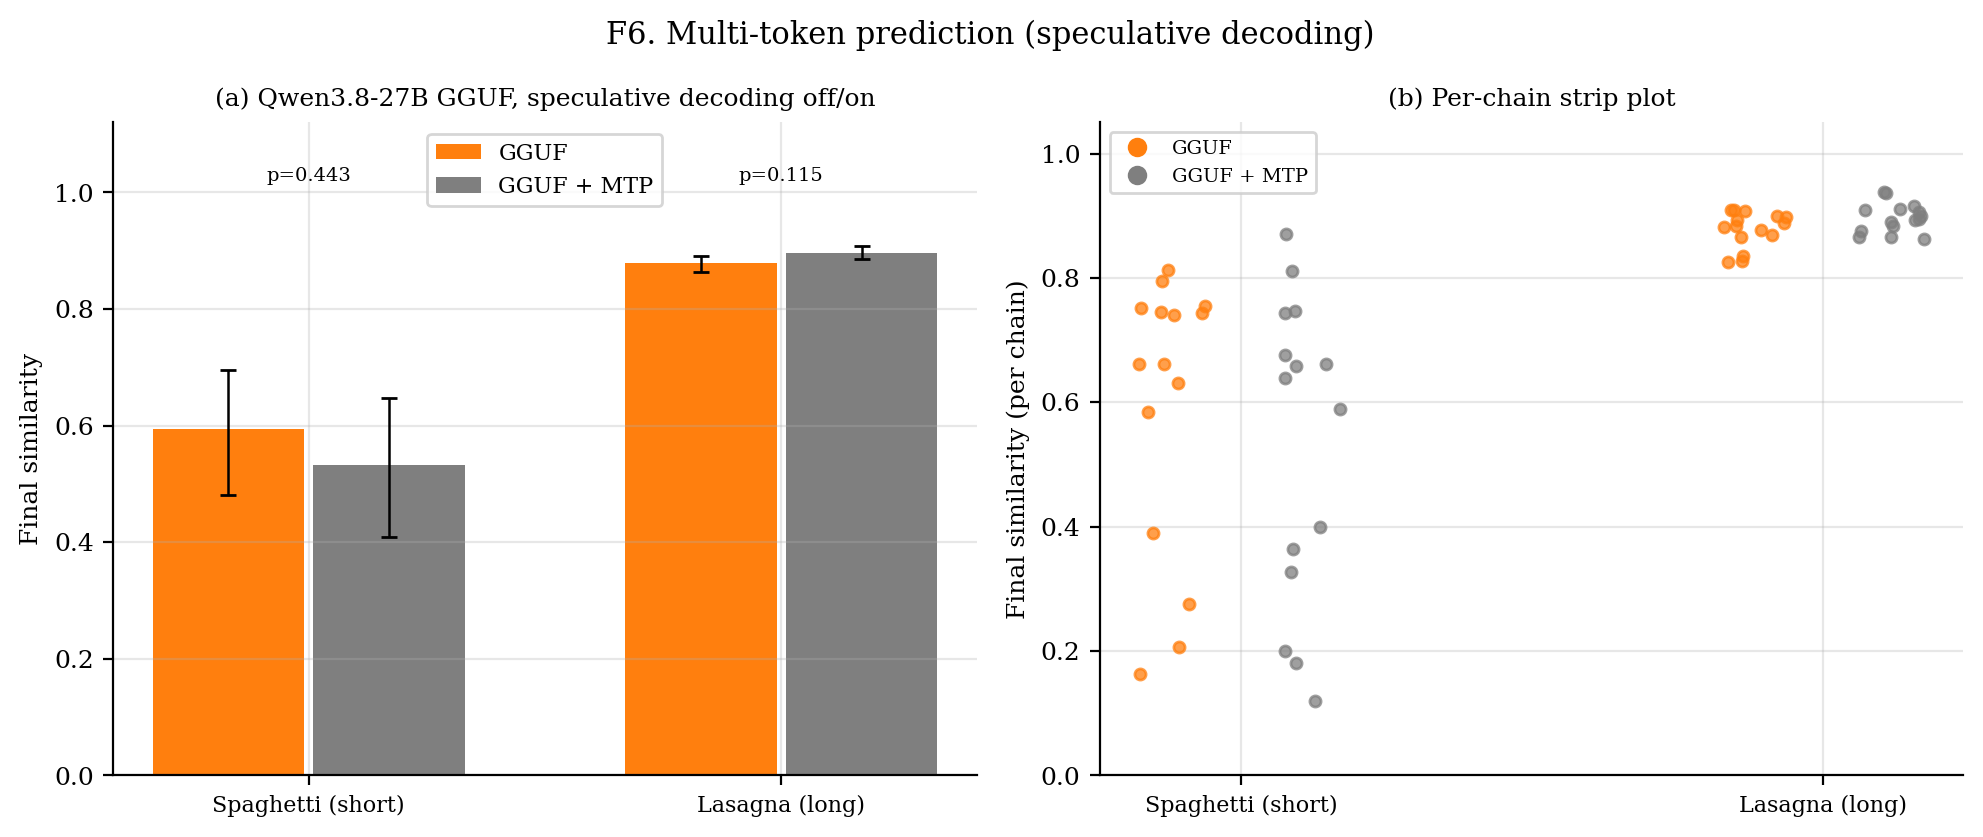
\includegraphics[width=0.85\textwidth,height=0.3\textheight,keepaspectratio]{../results/paper3_figures/fig6_mtp.png}
\caption{Multi-token-prediction speculative decoding on Qwen3.8-27B GGUF:
  per-chain final similarity with and without the draft head.}
\label{fig:mtp}
\end{figure}

\subsection{Temperature}
\label{sec:temperature}

Figure~\ref{fig:temperature} extends the temperature ablation to the new
models with 15 samples at $T=0$. The stable configuration, Qwen3.6-35B, is
flat within 0.05 across the range on both recipes and both hosts.
Qwen3.8-27B on spaghetti is U-shaped, 0.718 at $T=0$, falling to 0.582 at
$T=0.7$ and recovering to 0.747 at $T=1.0$, the same non-monotonic pattern
Paper~A reported for small Qwen3.5 models. Flash-Next declines with
temperature on lasagna (0.918 to 0.792). None of the three models is
improved by greedy decoding beyond the variance reduction described in
Section~\ref{sec:seeds}.

\begin{figure}[htbp]
\centering
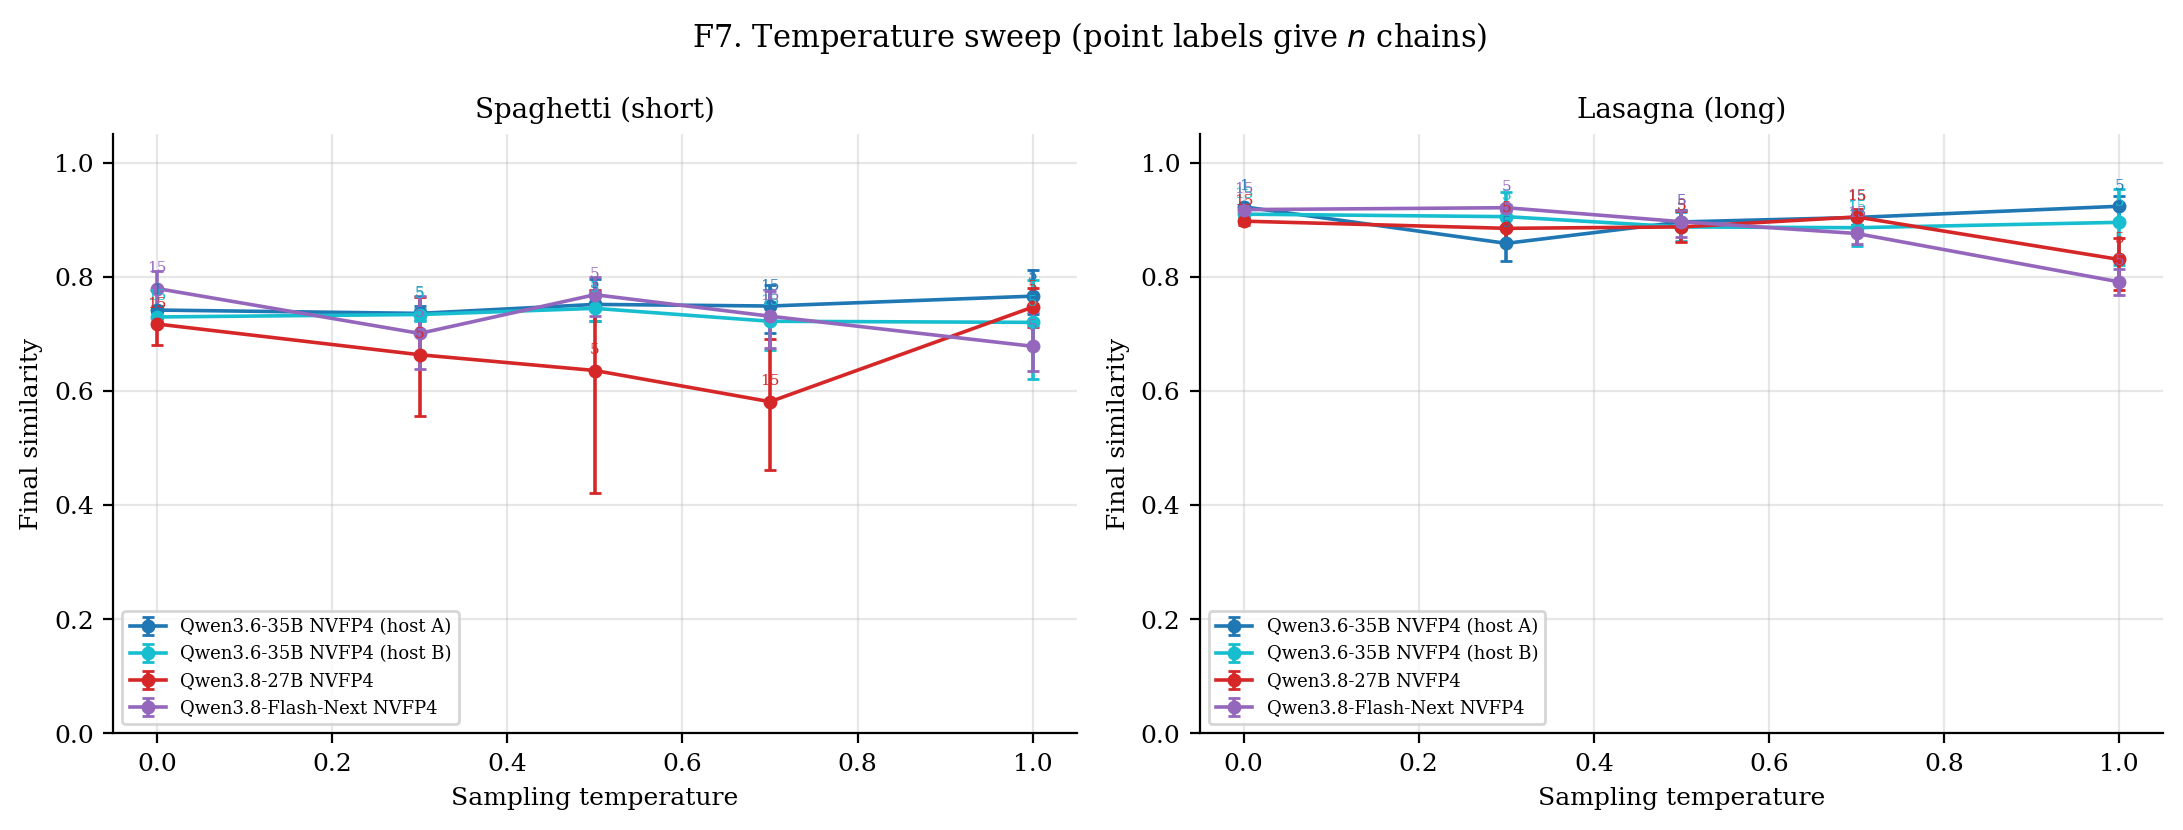
\includegraphics[width=\textwidth,height=0.3\textheight,keepaspectratio]{../results/paper3_figures/fig7_temperature.png}
\caption{Final similarity against temperature; $n$ per point in the
  legend. Both Qwen3.6-35B hosts are shown separately.}
\label{fig:temperature}
\end{figure}

\subsection{System prompts transfer within a generation}
\label{sec:sysprompt}

Paper~A found that prompt rankings did not transfer across families and
transferred only partially within Qwen3.5. Figure~\ref{fig:sysprompt} and
Table~\ref{tab:paper3-sysprompt} give a different answer for Qwen3.6 and
3.8. The effect is large everywhere: the spread between best and worst of
the 20 prompts is 0.24--0.43 on every configuration and both recipes, and
the complexity threshold of Paper~A, below which prompts were invisible on
the short stimulus, does not exist for these models. The rankings are also
stable. Across the two hosts they agree at $\rho=0.98$ (spaghetti) and
0.95 (lasagna); across models within the same recipe at 0.83--0.90 on
spaghetti and 0.70--0.88 on lasagna; and across recipes within a model at
only 0.25--0.58. A prompt ranking is thus a real, measurable property of a
model-and-stimulus pair, reproducible at five samples, and it is shared by
the models of this generation on a given stimulus.

The winners and losers are consistent. The anti-drift and constrained
categories score 0.86--0.95, the visually oriented prompts 0.65--0.78 on
every configuration, below the no-prompt baseline, and the best single
prompt is a fidelity instruction (100\% Fidelity, Ultra-Constrained
Fidelity or Precise Transmitter) on six of eight configuration--recipe
pairs, at 0.94--0.97. On Qwen3.8-27B spaghetti the worst prompt is no
prompt at all (0.672), because any instruction suppresses the menu-of-
options failure described in Section~\ref{sec:thinking}.

\begin{figure}[htbp]
\centering
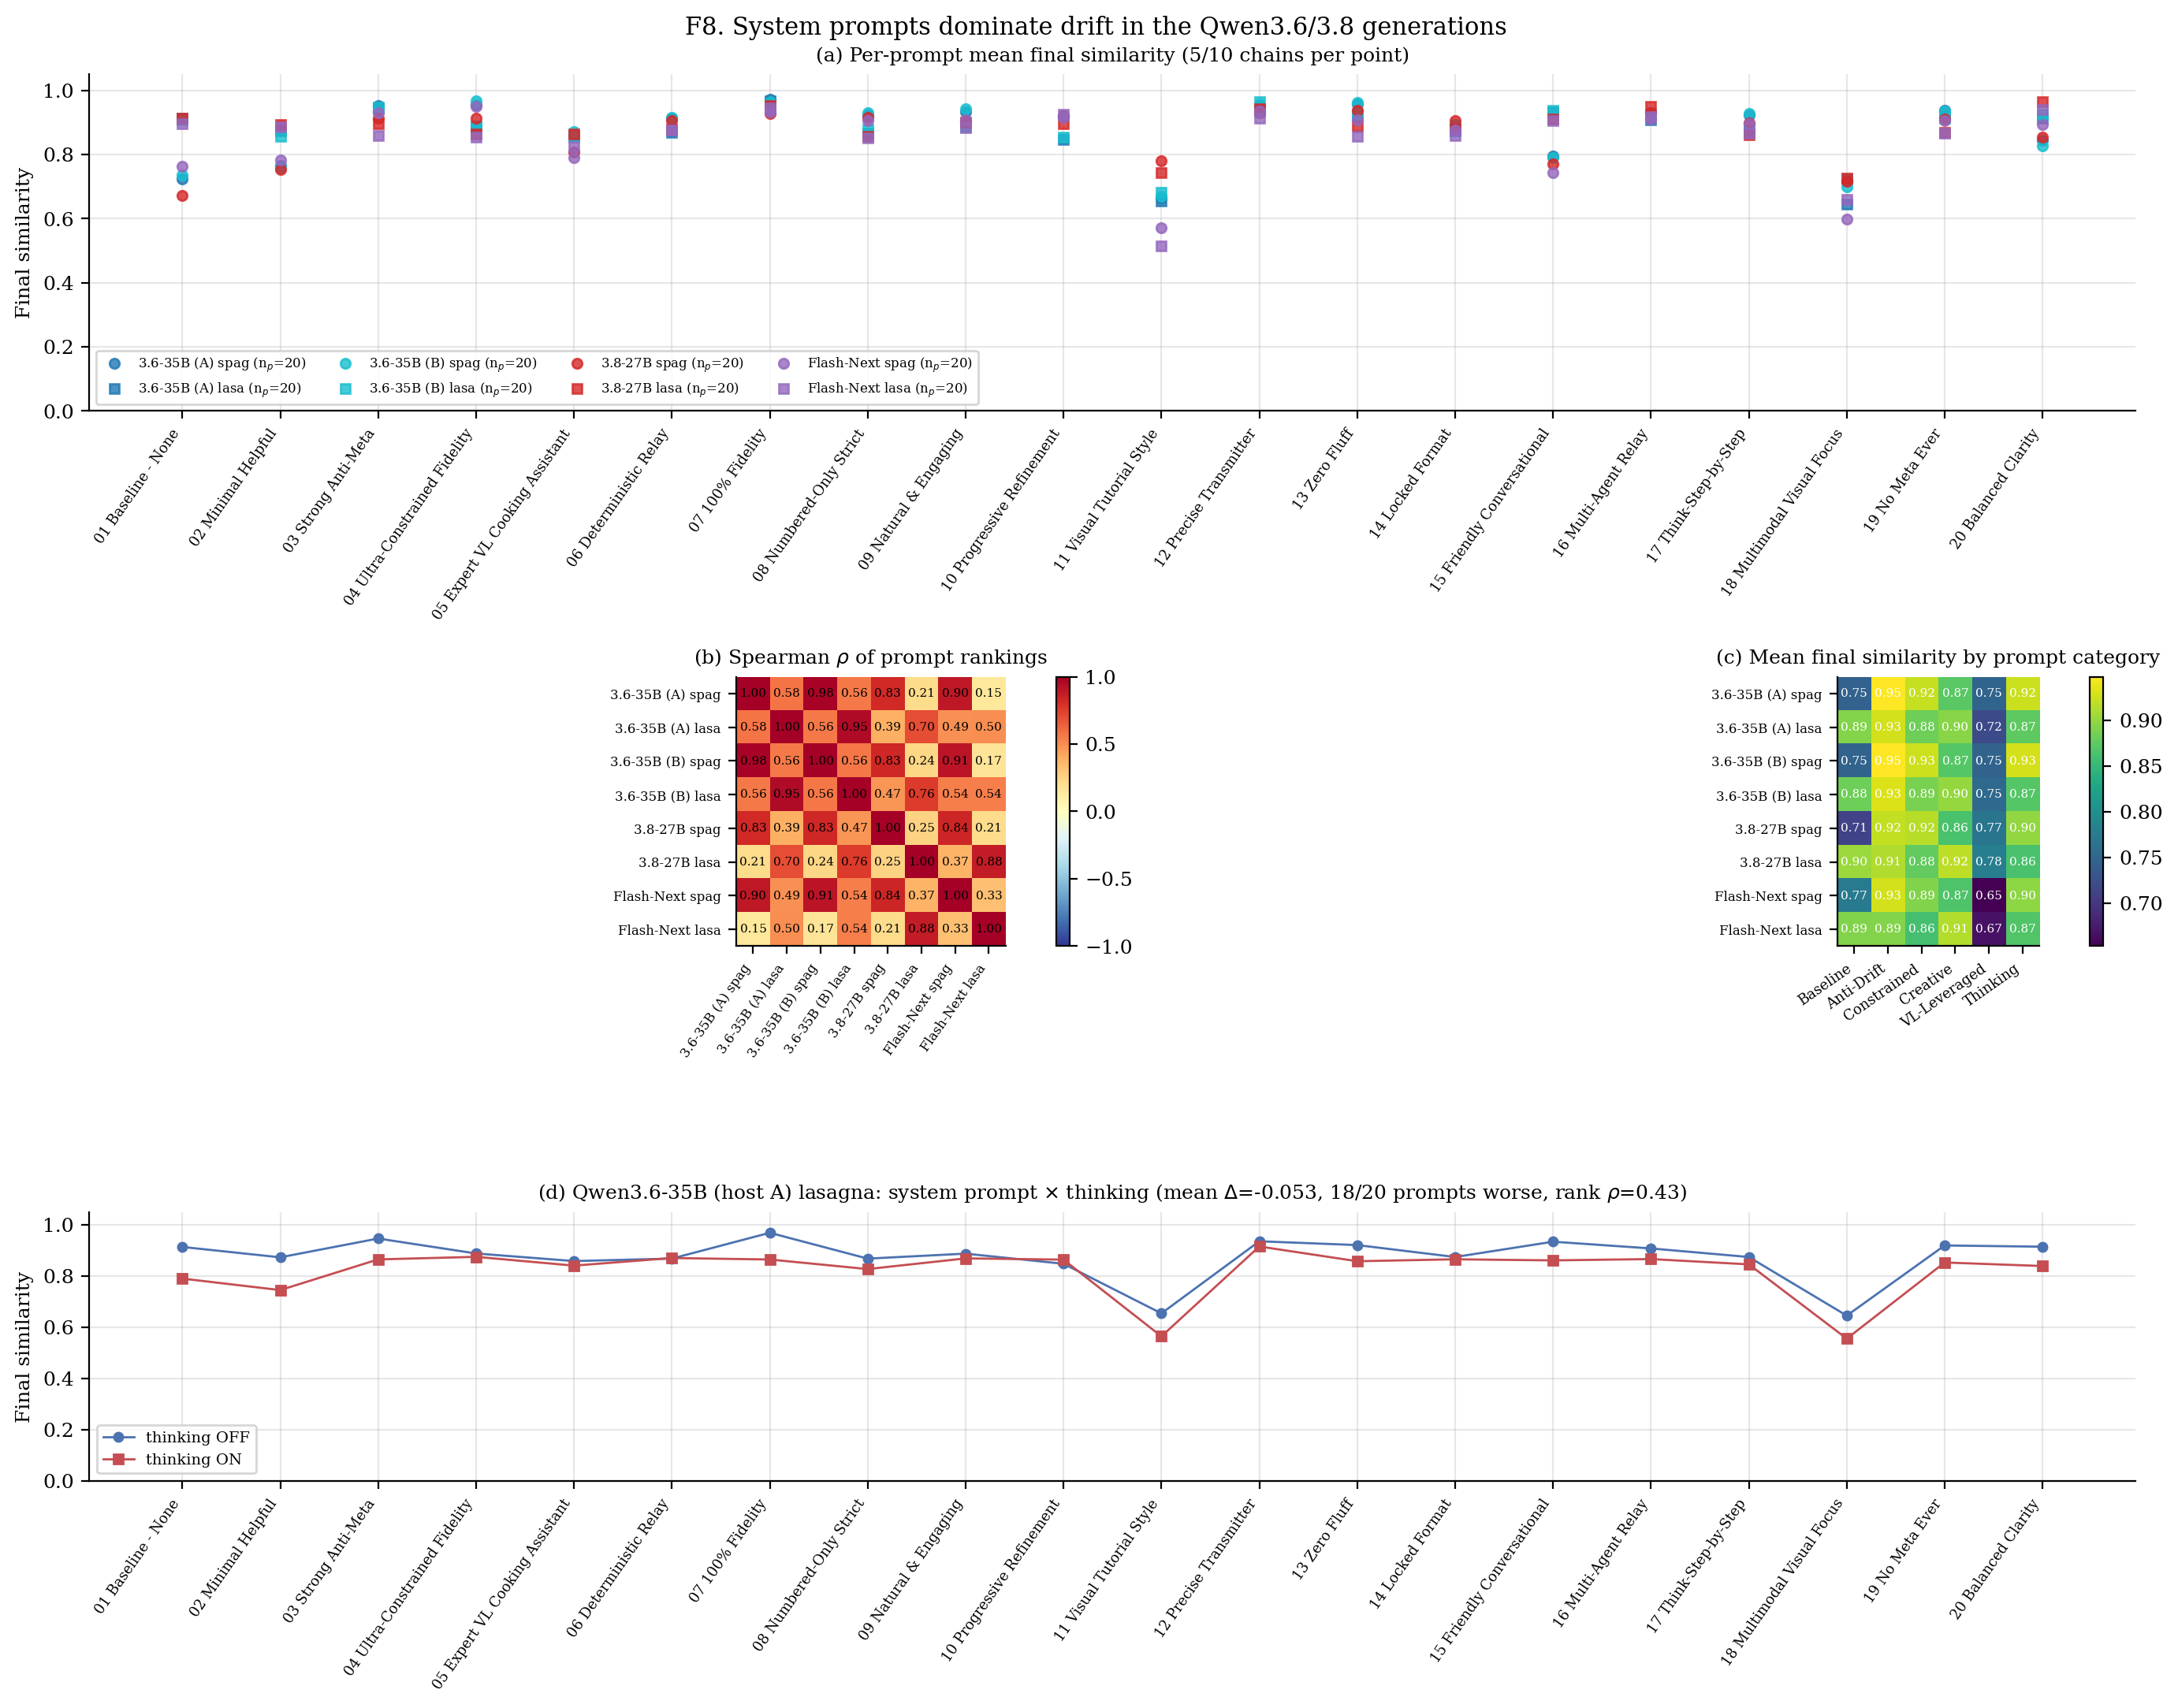
\includegraphics[width=\textwidth,height=0.42\textheight,keepaspectratio]{../results/paper3_figures/fig8_sysprompt.png}
\caption{System prompts. (a) Per-prompt final similarity, 20 prompts, four
  configurations, both recipes. (b) Spearman rank correlation between
  configuration--recipe pairs. (c) Category means. (d) Thinking off against
  on per prompt, Qwen3.6-35B lasagna.}
\label{fig:sysprompt}
\end{figure}

\begin{table}[t]
\centering
\caption{System-prompt sensitivity. Spread is the best minus the worst prompt mean
for that configuration and recipe; ``chains'' is the number of independent chains
behind each prompt mean. The lower block gives the
Spearman rank correlation of prompt orderings between every pair of
configuration$\times$recipe cells, with bootstrap 95\% CIs.}
\label{tab:paper3-sysprompt}
\resizebox{\textwidth}{!}{%
\begin{tabular}{llrrrll}
\toprule
Configuration & Recipe & prompts & chains & Spread & Best prompt & Worst prompt \\
\midrule
3.6-35B (A) & spaghetti & 20 & 10 & 0.306 & 100\% Fidelity (0.971) & Visual Tutorial Style (0.665) \\
3.6-35B (A) & lasagna & 20 & 5 & 0.323 & 100\% Fidelity (0.968) & Multimodal Visual Focus (0.645) \\
3.6-35B (B) & spaghetti & 20 & 5 & 0.298 & Ultra-Constrained Fidelity (0.967) & Visual Tutorial Style (0.669) \\
3.6-35B (B) & lasagna & 20 & 5 & 0.284 & Precise Transmitter (0.966) & Visual Tutorial Style (0.682) \\
3.8-27B & spaghetti & 20 & 5 & 0.266 & Zero Fluff (0.937) & Baseline - None (0.672) \\
3.8-27B & lasagna & 20 & 5 & 0.238 & Balanced Clarity (0.965) & Multimodal Visual Focus (0.727) \\
Flash-Next & spaghetti & 20 & 5 & 0.379 & Ultra-Constrained Fidelity (0.950) & Visual Tutorial Style (0.572) \\
Flash-Next & lasagna & 20 & 5 & 0.429 & 100\% Fidelity (0.945) & Visual Tutorial Style (0.516) \\
\bottomrule
\end{tabular}}

\vspace{1em}
\resizebox{\textwidth}{!}{%
\begin{tabular}{lrrlr}
\toprule
Pair & $n$ prompts & $\rho$ & 95\% CI & $p$ \\
\midrule
3.6-35B (A) spag vs 3.6-35B (A) lasa & 20 & 0.58 & [0.12, 0.86] & 0.0077 \\
3.6-35B (A) spag vs 3.6-35B (B) spag & 20 & 0.98 & [0.91, 1.00] & $<$0.0001 \\
3.6-35B (A) spag vs 3.6-35B (B) lasa & 20 & 0.56 & [0.15, 0.87] & 0.0103 \\
3.6-35B (A) spag vs 3.8-27B spag & 20 & 0.83 & [0.55, 0.94] & $<$0.0001 \\
3.6-35B (A) spag vs 3.8-27B lasa & 20 & 0.21 & [-0.31, 0.68] & 0.3695 \\
3.6-35B (A) spag vs Flash-Next spag & 20 & 0.90 & [0.68, 0.97] & $<$0.0001 \\
3.6-35B (A) spag vs Flash-Next lasa & 20 & 0.15 & [-0.42, 0.62] & 0.5352 \\
3.6-35B (A) lasa vs 3.6-35B (B) spag & 20 & 0.56 & [0.10, 0.84] & 0.0106 \\
3.6-35B (A) lasa vs 3.6-35B (B) lasa & 20 & 0.95 & [0.82, 0.98] & $<$0.0001 \\
3.6-35B (A) lasa vs 3.8-27B spag & 20 & 0.39 & [-0.09, 0.74] & 0.0923 \\
3.6-35B (A) lasa vs 3.8-27B lasa & 20 & 0.70 & [0.37, 0.88] & 0.0006 \\
3.6-35B (A) lasa vs Flash-Next spag & 20 & 0.49 & [-0.04, 0.82] & 0.0277 \\
3.6-35B (A) lasa vs Flash-Next lasa & 20 & 0.50 & [-0.06, 0.85] & 0.0261 \\
3.6-35B (B) spag vs 3.6-35B (B) lasa & 20 & 0.56 & [0.12, 0.86] & 0.0096 \\
3.6-35B (B) spag vs 3.8-27B spag & 20 & 0.83 & [0.56, 0.93] & $<$0.0001 \\
3.6-35B (B) spag vs 3.8-27B lasa & 20 & 0.24 & [-0.29, 0.67] & 0.3038 \\
3.6-35B (B) spag vs Flash-Next spag & 20 & 0.91 & [0.71, 0.98] & $<$0.0001 \\
3.6-35B (B) spag vs Flash-Next lasa & 20 & 0.17 & [-0.40, 0.66] & 0.4818 \\
3.6-35B (B) lasa vs 3.8-27B spag & 20 & 0.47 & [-0.02, 0.80] & 0.0369 \\
3.6-35B (B) lasa vs 3.8-27B lasa & 20 & 0.76 & [0.47, 0.89] & 0.0001 \\
3.6-35B (B) lasa vs Flash-Next spag & 20 & 0.54 & [0.05, 0.88] & 0.0140 \\
3.6-35B (B) lasa vs Flash-Next lasa & 20 & 0.54 & [0.06, 0.88] & 0.0137 \\
3.8-27B spag vs 3.8-27B lasa & 20 & 0.25 & [-0.25, 0.67] & 0.2855 \\
3.8-27B spag vs Flash-Next spag & 20 & 0.84 & [0.61, 0.93] & $<$0.0001 \\
3.8-27B spag vs Flash-Next lasa & 20 & 0.21 & [-0.32, 0.63] & 0.3660 \\
3.8-27B lasa vs Flash-Next spag & 20 & 0.37 & [-0.13, 0.77] & 0.1053 \\
3.8-27B lasa vs Flash-Next lasa & 20 & 0.88 & [0.67, 0.97] & $<$0.0001 \\
Flash-Next spag vs Flash-Next lasa & 20 & 0.33 & [-0.23, 0.74] & 0.1582 \\
\bottomrule
\end{tabular}}
\end{table}


\subsection{Byte-level locking}
\label{sec:locking}

Paper~A described fixed-point attractors as similarity plateaus. The saved
texts show something stronger. Figure~\ref{fig:locking} reports the fraction
of chains whose last three outputs are byte-identical: 87\% for Qwen3.6-35B
NVFP4 on both recipes, 93\% for Qwen3.8-27B NVFP4, 60--100\% for the GGUF
builds, with mean lock onset between iterations 3.5 and 9.5. At temperature
0.7 these models copy their input verbatim once it has been rewritten a few
times; ``paraphrase'' collapses into ``repeat'', and the final similarity
mostly records where the copying attractor caught the chain. Flash-Next is
the exception (20\% on spaghetti, 0\% on lasagna, onset at iteration 27
when it locks at all) and keeps rewriting to the end. With thinking on no
chain of any model locks, which is the mechanism behind the missing fixed
point of Section~\ref{sec:thinking}: a reasoning pass never reproduces its
input exactly.

\begin{figure}[htbp]
\centering
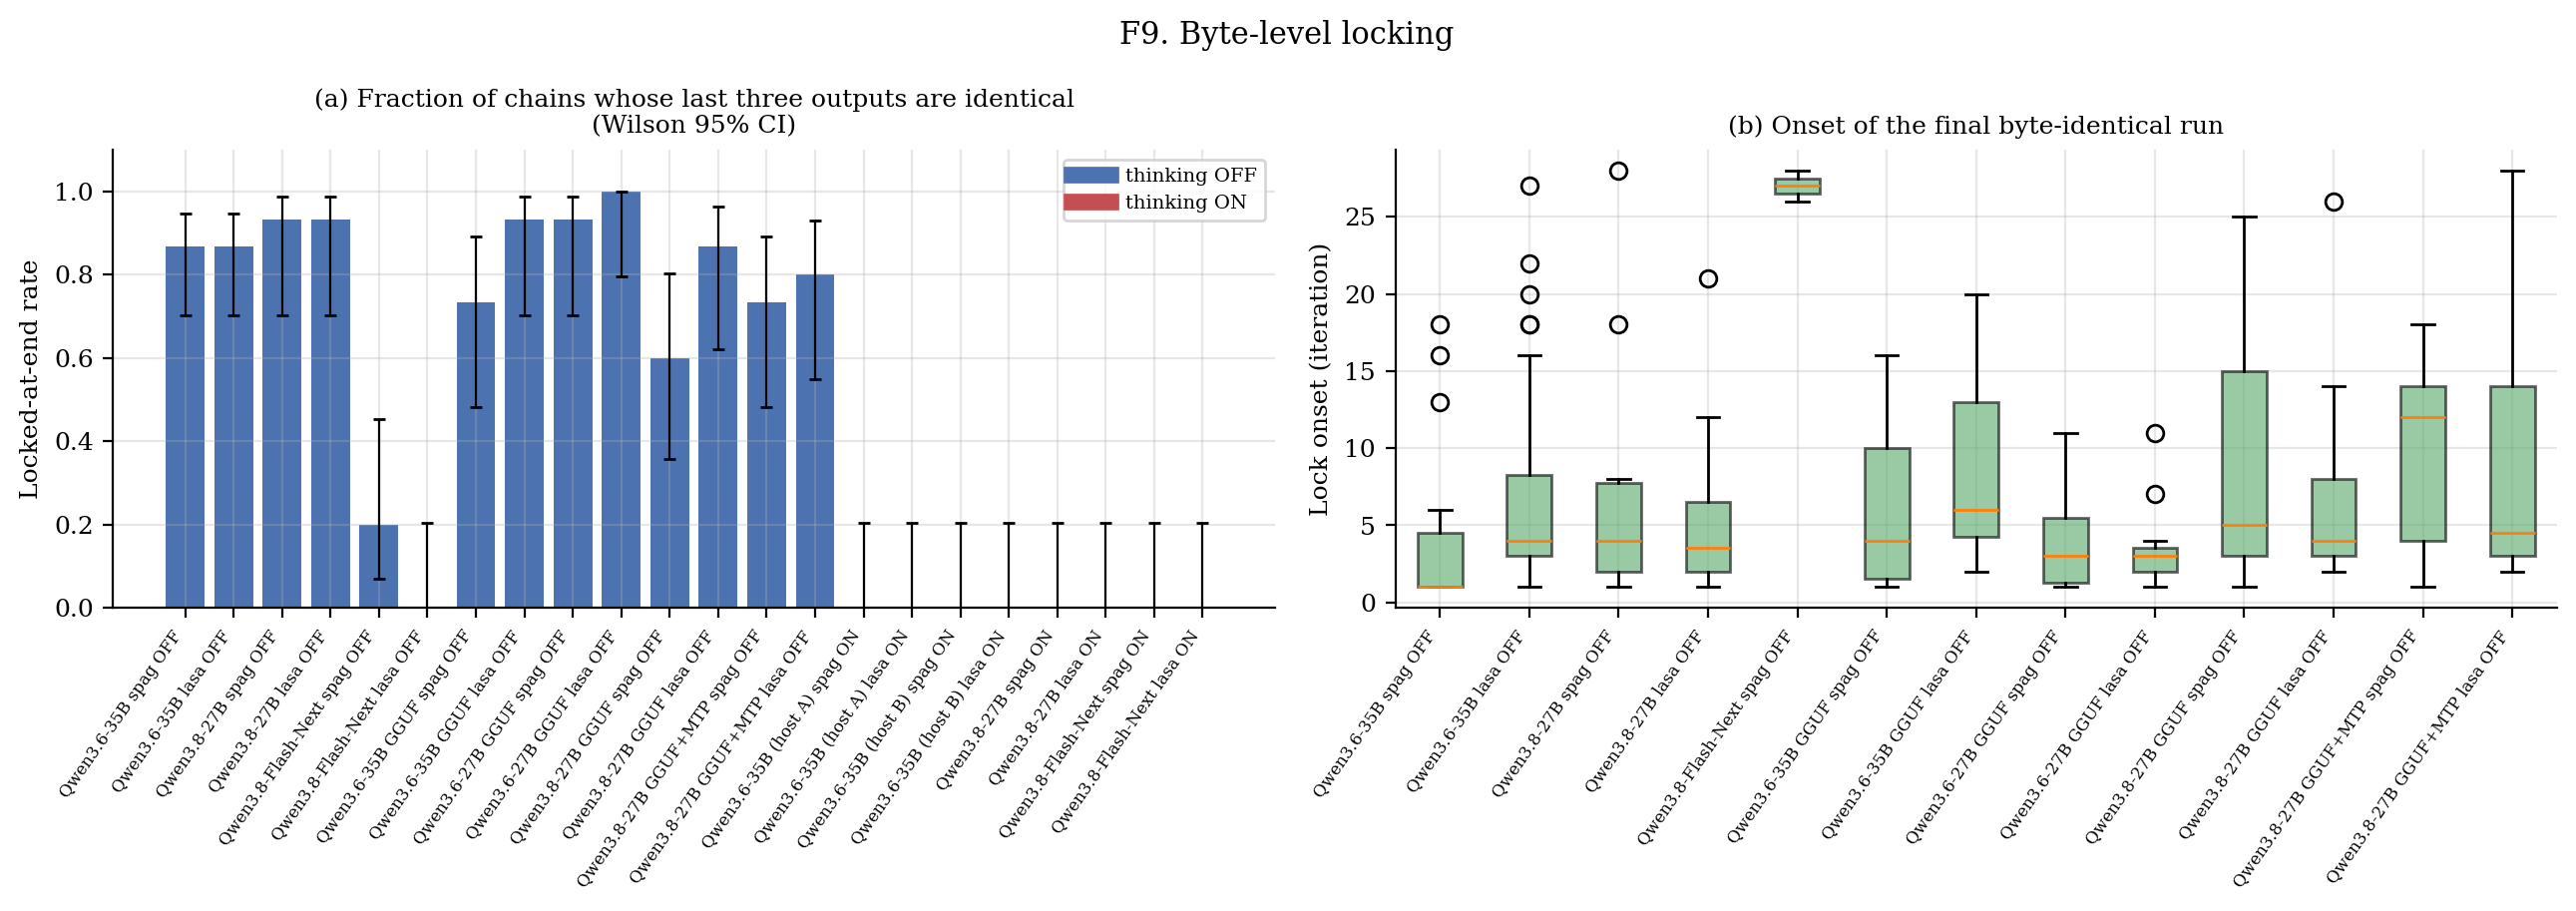
\includegraphics[width=\textwidth,height=0.3\textheight,keepaspectratio]{../results/paper3_figures/fig9_locking.png}
\caption{Locked-at-end rate with Wilson intervals, and lock-onset
  distribution, per configuration and recipe, thinking off and on.}
\label{fig:locking}
\end{figure}

\subsection{Construction statements of work: similarity against numbers}
\label{sec:concrete}

Table~\ref{tab:paper3-concrete} and Figure~\ref{fig:concrete} report the
first non-recipe stimulus. On the 95-word summary statement of work, all
three models finish at similarity 0.73--0.75, a value that in the recipe
data would indicate substantial drift. Yet every one of the document's
numeric tokens survives thirty paraphrases in essentially every chain
(numeric survival 0.998--1.000). What the similarity score is registering is
that the models inflate the document 2.3--2.4-fold and, in 60--100\% of
chains, reframe it as a memo or cover email to a project manager, with
placeholders for the sender's name; the quantities, specifications and
standards are all still there. On the 585-word detailed statement,
similarity is higher (0.81--0.85) while numeric survival is lower
(0.85--0.91), and the exclusions list, the clause a bidder must see, is
retained in 97--100\% of chains. Across the 120 baseline chains, similarity
and numeric survival are negatively correlated ($\rho=-0.42$, $p<0.001$),
and across all 270 concrete chains weakly so ($\rho=-0.18$). In this
domain the metric points the wrong way.

Thinking mode has a domain-specific cost that the similarity score hides.
With thinking on, similarity rises on every model (to 0.77--0.87), genre
drift disappears on the Qwen3.8 models, and the numbers still survive
(0.88--1.00); but the exclusions clause is dropped in 60--80\% of
short-document chains (retention 0.87 to 0.40 on Qwen3.6-35B, 0.80 to 0.20
on Qwen3.8-27B, 0.67 to 0.27 on Flash-Next). The reasoning pass tidies the
document and deletes the one line whose absence changes what the reader
would bid. The Ultra-Constrained Fidelity prompt, by contrast, gives 0.96
and 0.98 with every number, every exclusion and no reframing.

\begin{figure}[htbp]
\centering
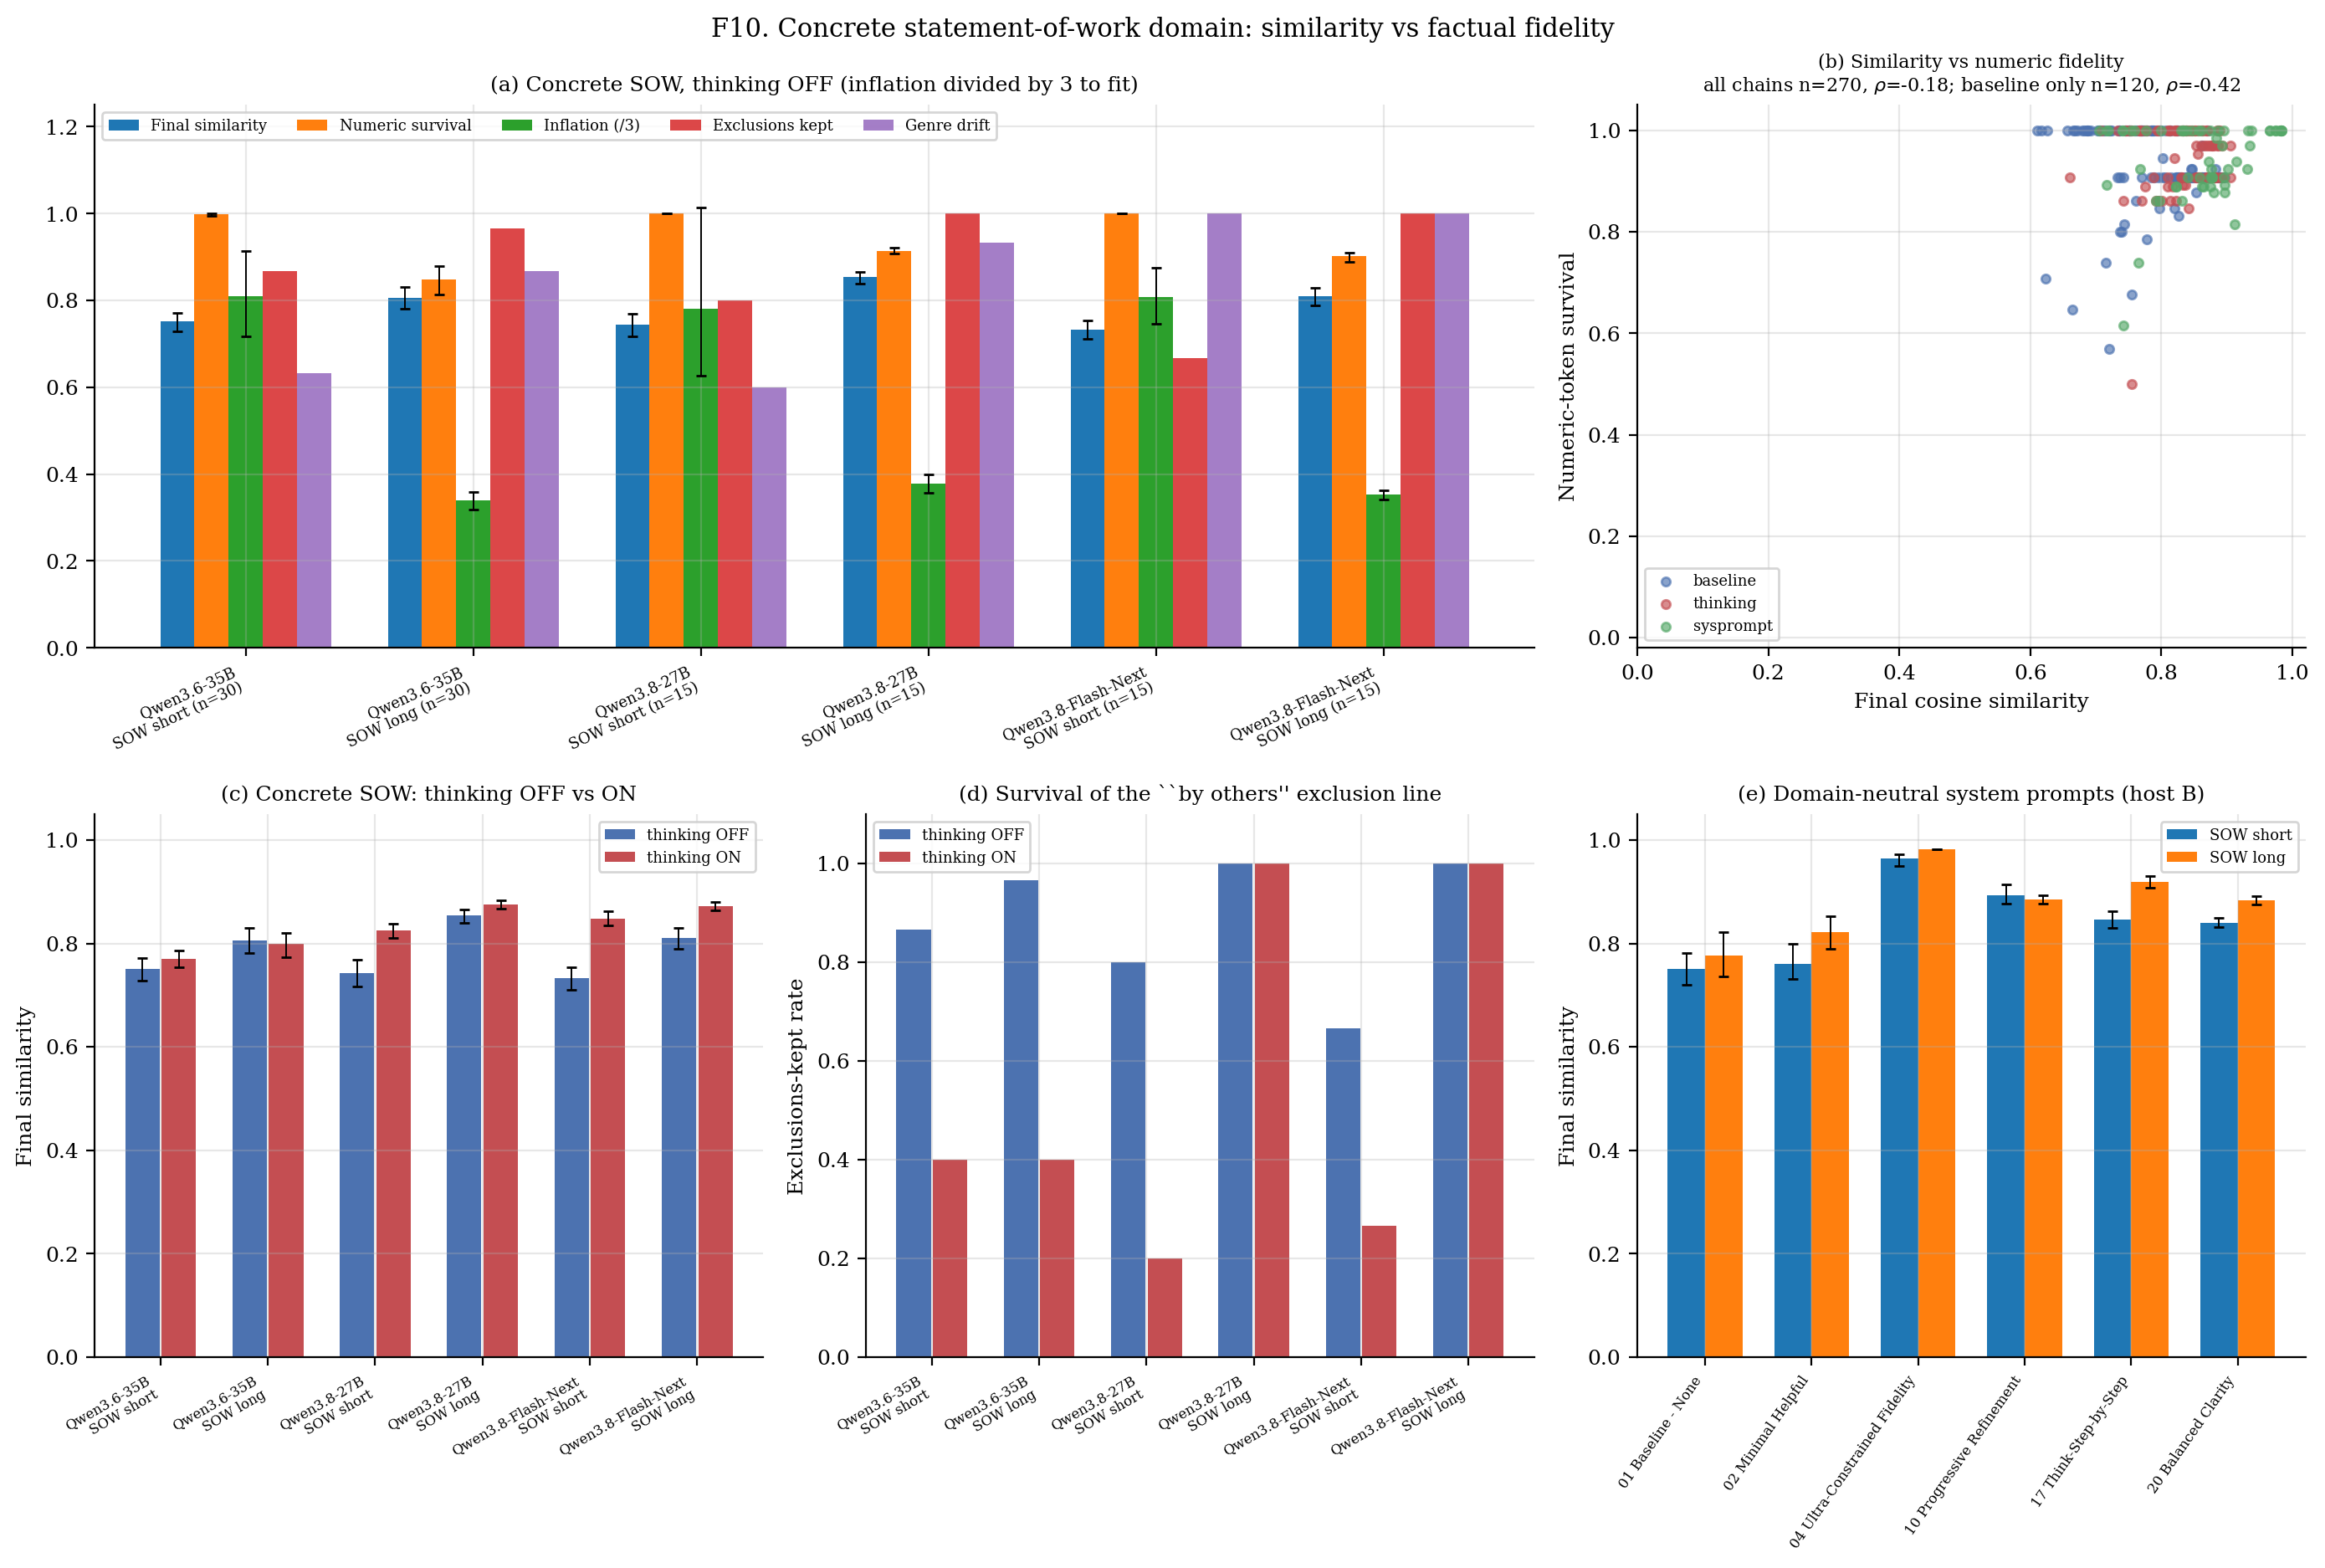
\includegraphics[width=\textwidth,height=0.42\textheight,keepaspectratio]{../results/paper3_figures/fig10_concrete.png}
\caption{Construction statements of work: final similarity, numeric-token
  survival, inflation, exclusion retention and genre drift, thinking off and
  on; the six domain-neutral prompts on host B; and similarity against
  numeric survival per chain.}
\label{fig:concrete}
\end{figure}

\begin{table}[t]
\centering
\caption{Construction statement-of-work domain. Numeric survival is the fraction of
the prompt's distinct numeric tokens still present in the iteration-30 output;
exclusions kept is the fraction of chains whose final output still contains the
``by others'' / ``exclusion'' language; genre drift is the fraction reframed as an
email or memo. The lower block is the domain-neutral system-prompt subset on host B.}
\label{tab:paper3-concrete}
\resizebox{\textwidth}{!}{%
\begin{tabular}{lllrrrrrr}
\toprule
Configuration & Document & Think & $n$ & Sim & Numeric & Inflation & Excl.\ kept & Genre drift \\
\midrule
Qwen3.6-35B NVFP4 & SOW short & OFF & 30 & 0.751 & 1.00 & 2.43 & 0.87 & 0.63 \\
Qwen3.6-35B NVFP4 & SOW long & OFF & 30 & 0.806 & 0.85 & 1.02 & 0.97 & 0.87 \\
Qwen3.8-27B NVFP4 & SOW short & OFF & 15 & 0.743 & 1.00 & 2.34 & 0.80 & 0.60 \\
Qwen3.8-27B NVFP4 & SOW long & OFF & 15 & 0.853 & 0.91 & 1.13 & 1.00 & 0.93 \\
Qwen3.8-Flash-Next NVFP4 & SOW short & OFF & 15 & 0.733 & 1.00 & 2.42 & 0.67 & 1.00 \\
Qwen3.8-Flash-Next NVFP4 & SOW long & OFF & 15 & 0.810 & 0.90 & 1.06 & 1.00 & 1.00 \\
Qwen3.6-35B NVFP4 & SOW short & ON & 15 & 0.770 & 1.00 & 2.47 & 0.40 & 0.40 \\
Qwen3.6-35B NVFP4 & SOW long & ON & 15 & 0.799 & 0.88 & 1.21 & 0.40 & 0.87 \\
Qwen3.8-27B NVFP4 & SOW short & ON & 15 & 0.825 & 0.95 & 1.69 & 0.20 & 0.00 \\
Qwen3.8-27B NVFP4 & SOW long & ON & 15 & 0.875 & 0.94 & 1.78 & 1.00 & 0.00 \\
Qwen3.8-Flash-Next NVFP4 & SOW short & ON & 15 & 0.848 & 0.99 & 1.45 & 0.27 & 0.00 \\
Qwen3.8-Flash-Next NVFP4 & SOW long & ON & 15 & 0.872 & 0.93 & 1.48 & 1.00 & 0.20 \\
\bottomrule
\end{tabular}}

\vspace{1em}
\resizebox{\textwidth}{!}{%
\begin{tabular}{llrrrrrr}
\toprule
System prompt & Document & $n$ & Sim & Numeric & Inflation & Excl.\ kept & Genre drift \\
\midrule
Baseline - None & SOW short & 5 & 0.750 & 1.00 & 2.94 & 1.00 & 0.60 \\
Minimal Helpful & SOW short & 5 & 0.760 & 1.00 & 2.79 & 0.80 & 1.00 \\
Ultra-Constrained Fidelity & SOW short & 5 & 0.964 & 1.00 & 1.06 & 1.00 & 0.00 \\
Progressive Refinement & SOW short & 5 & 0.893 & 0.98 & 1.04 & 0.40 & 0.00 \\
Think-Step-by-Step & SOW short & 5 & 0.846 & 0.91 & 1.22 & 0.00 & 0.00 \\
Balanced Clarity & SOW short & 5 & 0.840 & 1.00 & 1.56 & 1.00 & 0.00 \\
Baseline - None & SOW long & 5 & 0.776 & 0.80 & 0.92 & 1.00 & 1.00 \\
Minimal Helpful & SOW long & 5 & 0.821 & 0.89 & 1.17 & 1.00 & 0.80 \\
Ultra-Constrained Fidelity & SOW long & 5 & 0.982 & 1.00 & 1.05 & 1.00 & 0.00 \\
Progressive Refinement & SOW long & 5 & 0.885 & 0.91 & 0.80 & 1.00 & 0.00 \\
Think-Step-by-Step & SOW long & 5 & 0.919 & 0.91 & 0.93 & 1.00 & 0.00 \\
Balanced Clarity & SOW long & 5 & 0.883 & 0.92 & 1.10 & 1.00 & 0.00 \\
\bottomrule
\end{tabular}}
\end{table}


\subsection{Sixteen domains: what survives and what the metric sees}
\label{sec:breadth}

Table~\ref{tab:paper3-breadth}, Table~\ref{tab:paper3-facttype} and
Figure~\ref{fig:breadth} give the breadth experiment on Qwen3.6-35B at 30
samples per domain. Final similarity is remarkably insensitive to domain,
spanning only 0.72 (literary prose) to 0.86 (discharge instructions), all
below the lasagna recipe's 0.90. Anchor-fact survival spans three times that
range: 0.30 for the laboratory protocol and 0.33 for literary prose, 0.43
for the change order and 0.49 for the financial summary, up to 0.91--0.93
for the travel itinerary, construction RFI and contract clause. At chain
level similarity and survival correlate at $\rho=0.32$; at domain level at
0.37 with an interval including zero. The laboratory protocol keeps 30\% of
its facts at similarity 0.81; the contract clause keeps 93\% at 0.84. A
score of 0.8 can mean that the document is intact or that most of what it
said is gone.

The domain ranking is real: it replicates across hosts at $\rho=0.95$ on
both metrics and transfers to Flash-Next at 0.77--0.78. By fact type
(Table~\ref{tab:paper3-facttype}), identifiers (0.81) and names (0.80)
survive best, numbers with units worse (0.63), and dates worst of all
(0.35): the financial summary lost every date in every chain and the change
order kept 13\%. Meta-commentary framing is present in 70--97\% of final
outputs in every domain, inflation runs 1.1--1.9 fold, and 53--93\% of chains
end locked.

Thinking on has no net effect across domains (0.772 against 0.792,
$p=0.29$) but reduces anchor survival (0.60 against 0.68) and is
destructive on the two domains where it matters most, literary prose
($-0.20$) and the recipe ($-0.15$). The Ultra-Constrained Fidelity prompt,
one domain-neutral sentence, raises similarity to 0.95 and anchor survival
to 0.97 across the sixteen domains, improving every one of them
($p<10^{-6}$), with inflation 1.05 and meta-commentary in 6\% of outputs. A
30-step paraphrase chain on this model is close to lossless in every domain
tested when told, in plain terms, to be.

\begin{figure}[htbp]
\centering
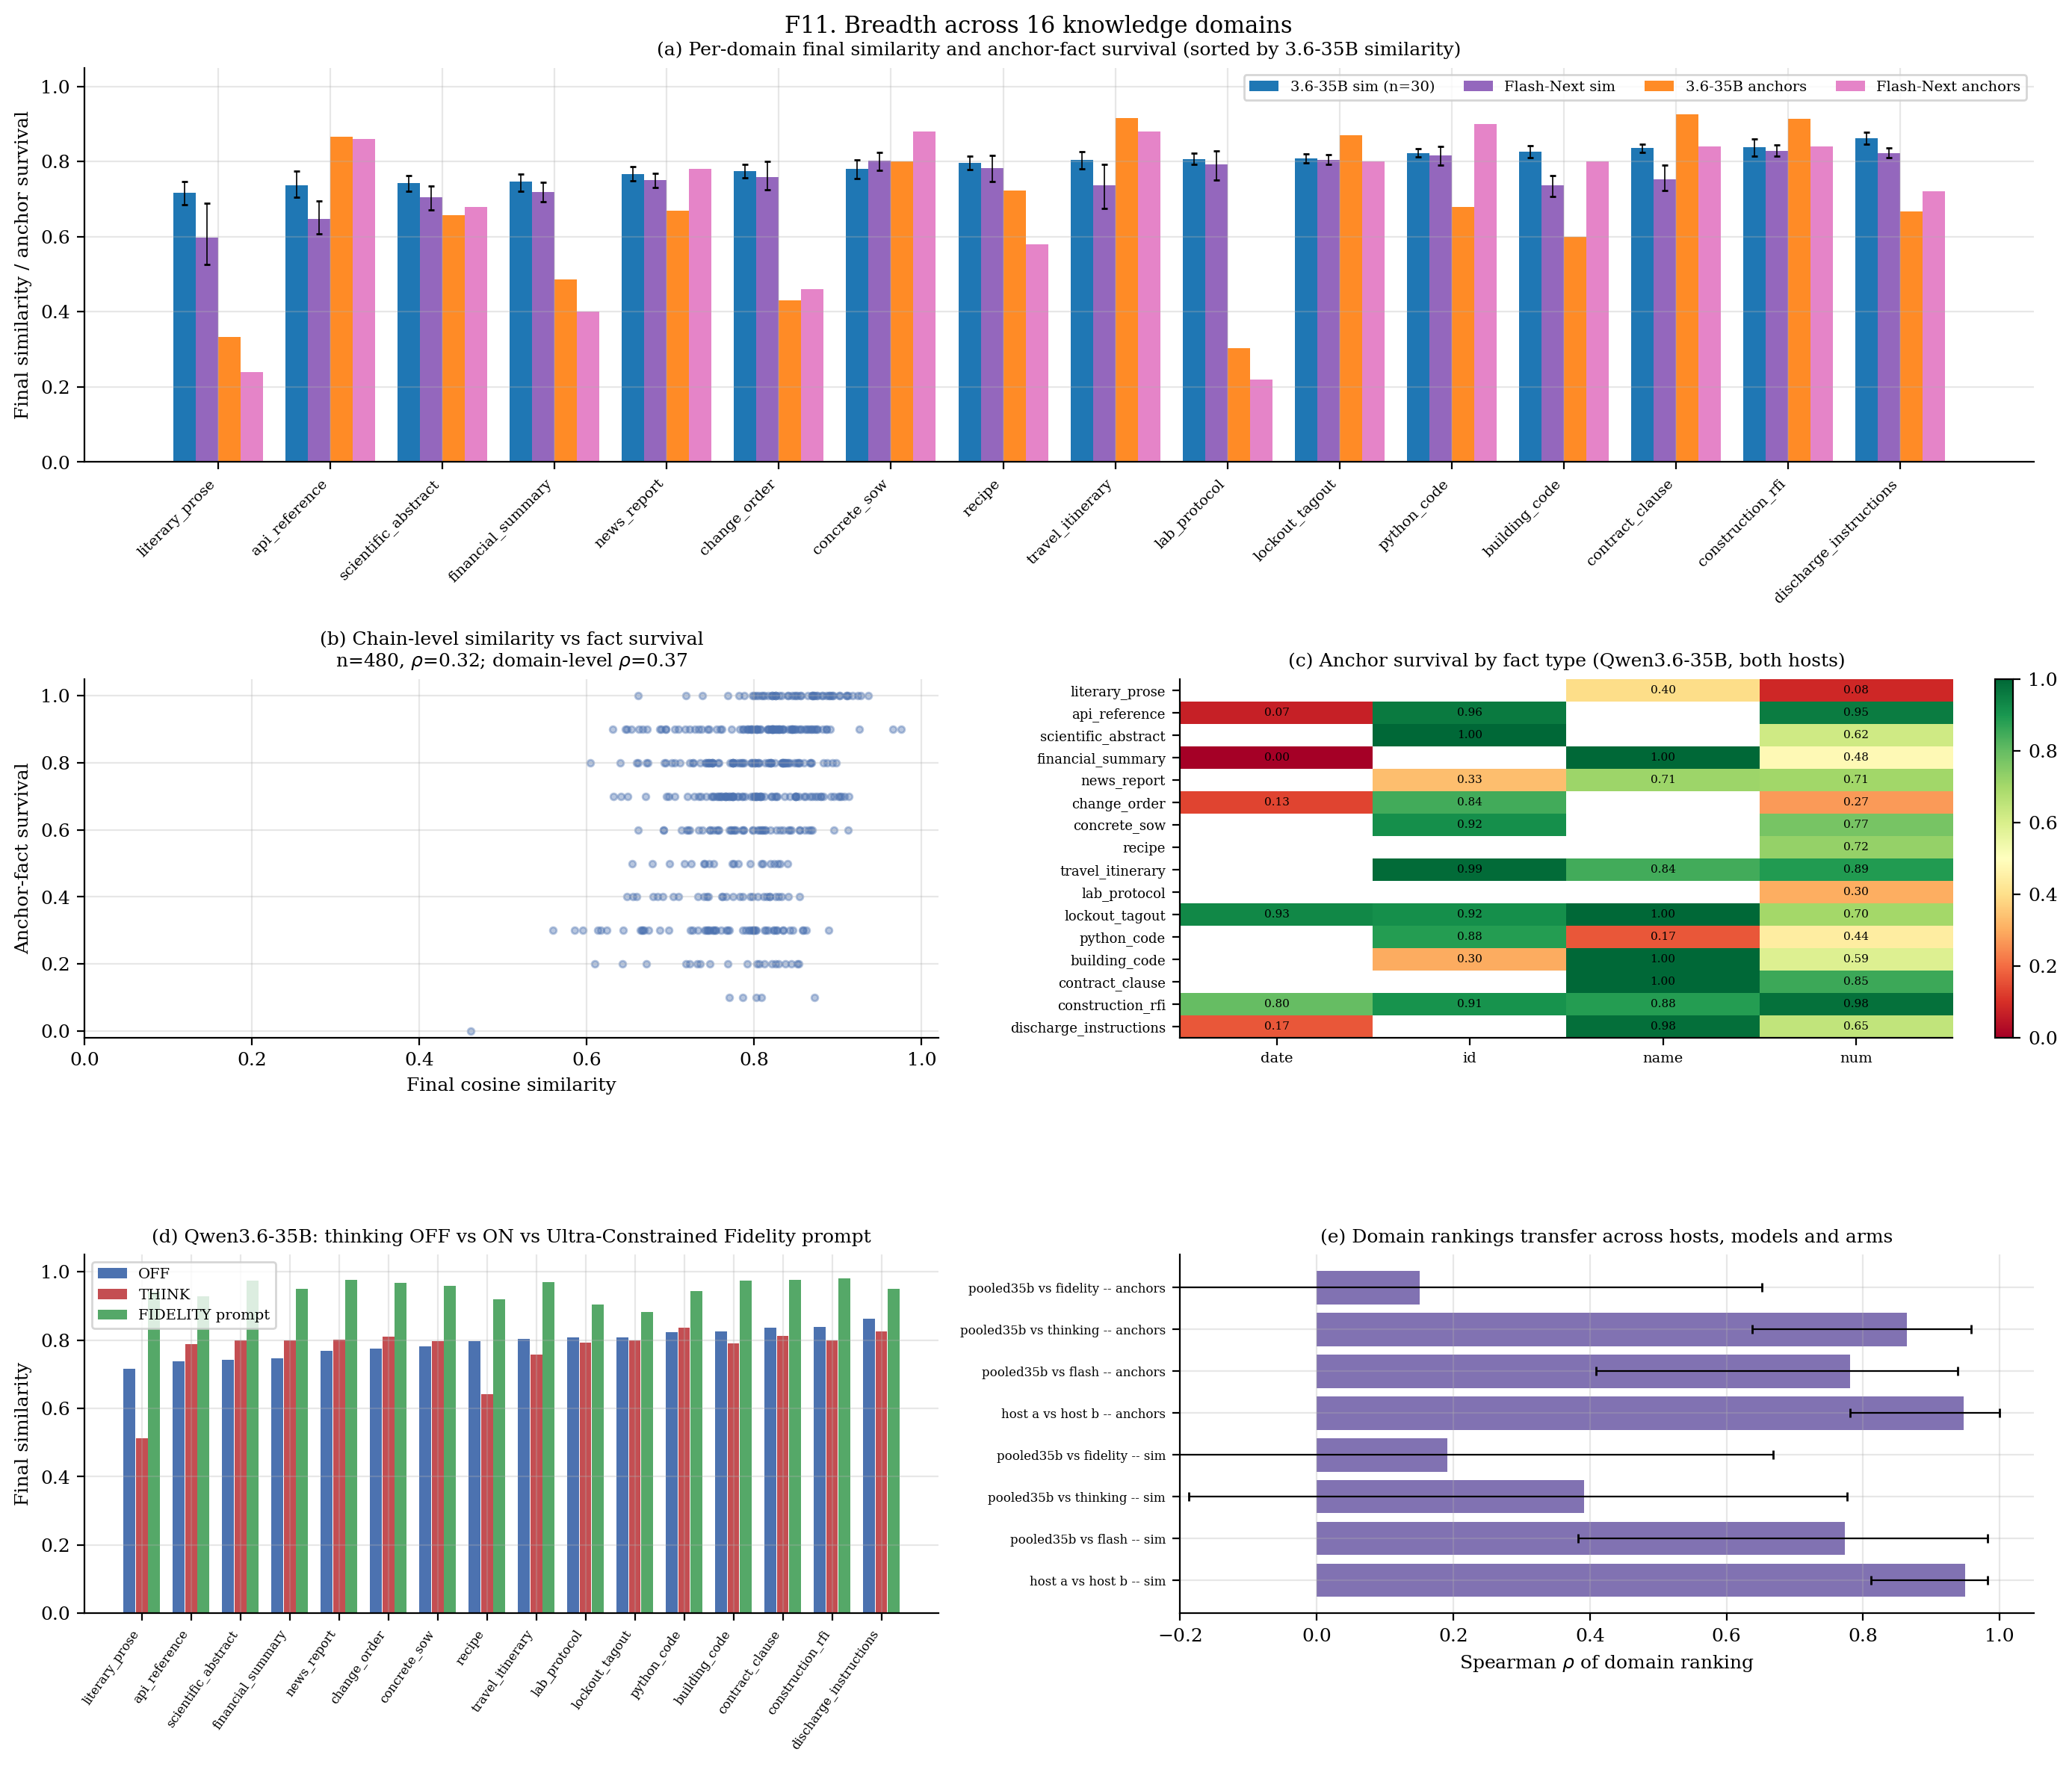
\includegraphics[width=\textwidth,height=0.48\textheight,keepaspectratio]{../results/paper3_figures/fig11_breadth.png}
\caption{Sixteen domains on Qwen3.6-35B (30 samples per domain, both
  hosts) and Flash-Next (5). (a) Final similarity and anchor-fact survival
  per domain. (b) Similarity against survival per chain. (c) Survival by
  fact type. (d) Thinking off, thinking on, and the fidelity prompt per
  domain.}
\label{fig:breadth}
\end{figure}

\begin{table}[t]
\centering
\caption{Breadth experiment, 16 knowledge domains, 30 iterations. The first block is
Qwen3.6-35B NVFP4 with both hosts pooled and thinking OFF; THINK is thinking ON,
FIDELITY is the domain-neutral Ultra-Constrained Fidelity system prompt, and Flash
is Qwen3.8-Flash-Next NVFP4. Anchors = fraction of the 10 anchor facts surviving
verbatim in the final output.}
\label{tab:paper3-breadth}
\resizebox{\textwidth}{!}{%
\begin{tabular}{lrrlrrrrrrr}
\toprule
Domain & $n$ & Sim & 95\% CI & Anchors & Infl. & Meta & Locked & THINK & FIDELITY & Flash \\
\midrule
discharge\_instructions & 30 & 0.862 & [0.846, 0.877] & 0.67 & 1.14 & 0.70 & 0.83 & 0.826 & 0.949 & 0.823 \\
construction\_rfi & 30 & 0.838 & [0.814, 0.860] & 0.91 & 1.34 & 0.93 & 0.83 & 0.798 & 0.980 & 0.829 \\
contract\_clause & 30 & 0.836 & [0.825, 0.847] & 0.93 & 1.30 & 0.93 & 0.90 & 0.812 & 0.977 & 0.752 \\
building\_code & 30 & 0.826 & [0.810, 0.842] & 0.60 & 1.22 & 0.87 & 0.83 & 0.790 & 0.973 & 0.737 \\
python\_code & 30 & 0.823 & [0.813, 0.833] & 0.68 & 1.86 & 0.87 & 0.80 & 0.835 & 0.943 & 0.817 \\
lockout\_tagout & 30 & 0.808 & [0.795, 0.821] & 0.87 & 1.27 & 0.77 & 0.83 & 0.798 & 0.882 & 0.805 \\
lab\_protocol & 30 & 0.807 & [0.792, 0.822] & 0.30 & 1.62 & 0.70 & 0.57 & 0.792 & 0.905 & 0.792 \\
travel\_itinerary & 30 & 0.804 & [0.781, 0.827] & 0.92 & 1.58 & 0.93 & 0.73 & 0.758 & 0.970 & 0.736 \\
recipe & 30 & 0.797 & [0.779, 0.814] & 0.72 & 1.53 & 0.80 & 0.70 & 0.642 & 0.920 & 0.783 \\
concrete\_sow & 30 & 0.780 & [0.756, 0.804] & 0.80 & 1.65 & 0.83 & 0.83 & 0.796 & 0.958 & 0.802 \\
change\_order & 30 & 0.774 & [0.756, 0.792] & 0.43 & 1.20 & 0.90 & 0.67 & 0.809 & 0.968 & 0.759 \\
news\_report & 30 & 0.767 & [0.749, 0.786] & 0.67 & 1.27 & 0.80 & 0.93 & 0.802 & 0.976 & 0.751 \\
financial\_summary & 30 & 0.746 & [0.721, 0.767] & 0.49 & 1.43 & 0.83 & 0.60 & 0.799 & 0.951 & 0.719 \\
scientific\_abstract & 30 & 0.742 & [0.721, 0.763] & 0.66 & 1.39 & 0.83 & 0.83 & 0.799 & 0.975 & 0.705 \\
api\_reference & 30 & 0.737 & [0.704, 0.774] & 0.87 & 1.61 & 0.87 & 0.80 & 0.788 & 0.928 & 0.647 \\
literary\_prose & 30 & 0.716 & [0.684, 0.748] & 0.33 & 1.30 & 0.97 & 0.53 & 0.512 & 0.941 & 0.598 \\
\bottomrule
\end{tabular}}
\end{table}


\begin{table}[t]
\centering
\caption{Anchor-fact survival by fact type (Qwen3.6-35B NVFP4, both hosts pooled,
thinking OFF, $n$=30 chains per domain). Each domain prompt carries exactly ten
tagged anchor facts.}
\label{tab:paper3-facttype}
\resizebox{\textwidth}{!}{%
\begin{tabular}{lrrrr}
\toprule
Domain & date & id & name & num \\
\midrule
api\_reference & 0.07 & 0.96 & --- & 0.95 \\
building\_code & --- & 0.30 & 1.00 & 0.59 \\
change\_order & 0.13 & 0.84 & --- & 0.27 \\
concrete\_sow & --- & 0.92 & --- & 0.77 \\
construction\_rfi & 0.80 & 0.91 & 0.88 & 0.98 \\
contract\_clause & --- & --- & 1.00 & 0.85 \\
discharge\_instructions & 0.17 & --- & 0.98 & 0.65 \\
financial\_summary & 0.00 & --- & 1.00 & 0.48 \\
lab\_protocol & --- & --- & --- & 0.30 \\
literary\_prose & --- & --- & 0.40 & 0.08 \\
lockout\_tagout & 0.93 & 0.92 & 1.00 & 0.70 \\
news\_report & --- & 0.33 & 0.71 & 0.71 \\
python\_code & --- & 0.88 & 0.17 & 0.44 \\
recipe & --- & --- & --- & 0.72 \\
scientific\_abstract & --- & 1.00 & --- & 0.62 \\
travel\_itinerary & --- & 0.99 & 0.84 & 0.89 \\
\midrule
\textbf{All domains} & 0.35 & 0.81 & 0.80 & 0.63 \\
\bottomrule
\end{tabular}}
\end{table}


\begin{figure}[htbp]
\centering
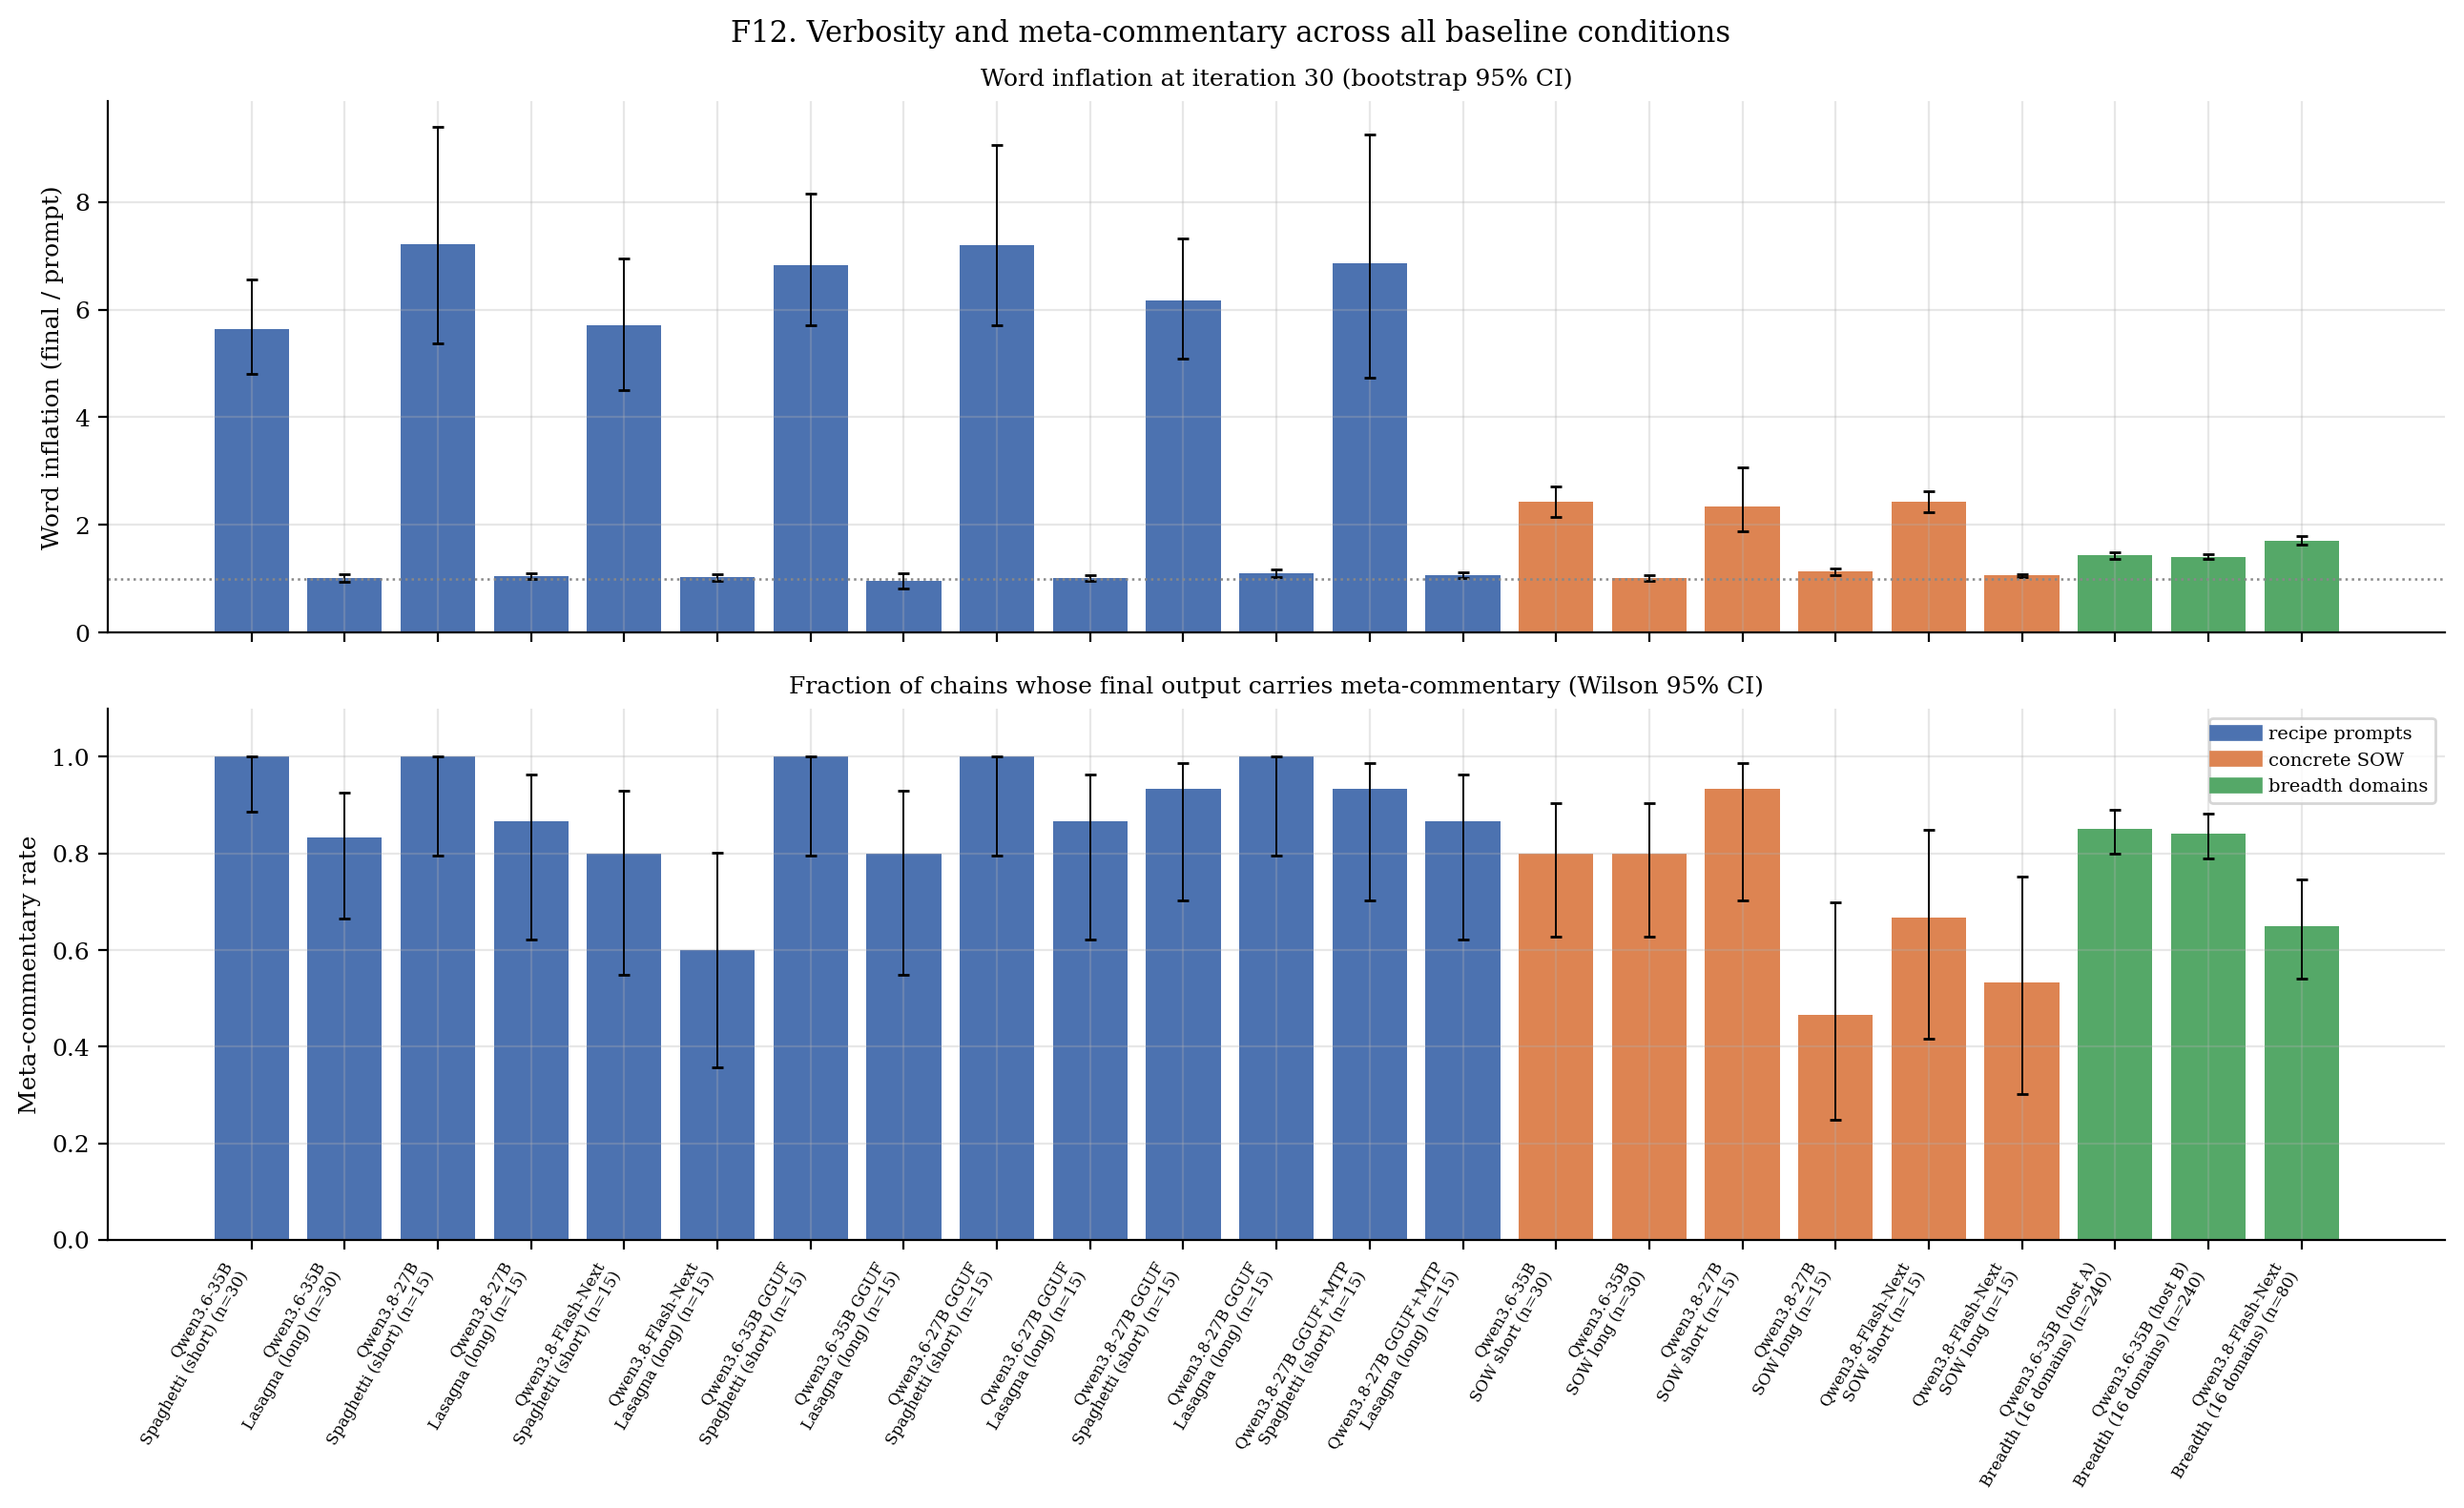
\includegraphics[width=\textwidth,height=0.3\textheight,keepaspectratio]{../results/paper3_figures/fig12_inflation_meta.png}
\caption{Word-count inflation and meta-commentary rate across every
  baseline condition: recipes, statements of work and the sixteen domains.}
\label{fig:inflation}
\end{figure}

\section{Discussion}
\label{sec:discussion}

\paragraph{What the similarity score measures.}
Three results converge. On the recipes, the short stimulus drifts far more
than the long one while inflating five- to seven-fold and acquiring
framing in nearly every chain. On the statements of work, similarity is
anti-correlated with the survival of the numbers. Across sixteen domains,
similarity varies by 0.14 while fact survival varies by 0.63, and the two
are only weakly related. Cosine similarity to the original, the metric of
Paper~A and of most of the iterated-generation literature, responds first
to length and genre change and only secondarily to information loss.
\citet{belem2026certainty} found one axis of change it cannot see;
Figure~\ref{fig:inflation} shows that it over-reads another. The
quantitative claims of Paper~A about which model drifts least survive
this---rankings replicate across metrics at $\rho\approx0.8$ where we can
compare them---but the interpretation of a value of 0.75 as ``25\% of the
meaning lost'' does not. We recommend that iterated-generation studies
report a fact-survival measure beside any embedding score, and we release
every chain's text so that they can.

\paragraph{The hierarchy, revised again.}
Paper~A ordered the factors governing drift as model family, then size to a
threshold, then a discrete failure mode, then quantization format, then
temperature and KV precision, with prompts as a multiplier. On the newer
generations the ordering within a deployed model is: thinking mode (0.03--
0.30, sign by model) and system prompt (0.24--0.43 spread) at the top,
format-and-stack next (0 to 0.16), and temperature, seed and speculative
decoding at or below the 0.05 noise floor. The two largest levers are the
two that a pipeline designer sets in software after the model is chosen,
and both are cheap to test at fifteen samples on these models.

\paragraph{Reasoning models in loops.}
The thinking results are, we think, the most consequential for practice. A
reasoning pass makes Qwen3.8 a better paraphraser and Qwen3.6 a worse one;
it prevents the copying attractor that otherwise ends most chains, so a
loop containing a reasoning model does not settle; it deletes a bidder's
exclusions clause in most short statements of work while raising the
similarity score; and on the previous generation it consumed the entire
generation budget in a seventh of all chains. None of these effects is
visible in a single-pass benchmark, and none is predictable from the model's
single-pass quality. A pipeline that iterates over a reasoning model should
be tested as a loop, with thinking on and off, on its own documents, with
a fact-level check.

\paragraph{Recommendations.}
\begin{enumerate}[leftmargin=*]
  \item Report iterated-generation results as samples, never as seeded
        replicates; fifteen chains per condition is a practical minimum.
  \item Test thinking mode in both states on the deployed model and
        stimulus; do not assume its sign.
  \item Use a fidelity instruction. One sentence lifted every domain tested
        to 0.88--0.98 with 97\% of facts intact.
  \item Measure fact survival, and check dates and quantities specifically;
        they are the first things lost.
  \item Do not spend effort on seeds, greedy decoding or speculative
        decoding as drift controls; they do not change the outcome.
  \item Benchmark the exact build and stack; the format effect is real on
        one of two models and absent on the other.
\end{enumerate}

\paragraph{Limitations.}
\begin{itemize}[leftmargin=*]
  \item \textbf{One family, four models.} Every configuration is a Qwen
        instruct model. The cross-generation trend is a within-family
        observation, and the Qwen3.5 anchors on the short stimulus rest on
        two or three clean chains.
  \item \textbf{Format confounds.} The GGUF arm differs from the NVFP4 arm
        in quantization, server, KV precision and GPU generation; the
        contrast bounds their combined effect.
  \item \textbf{Anchor facts are hand-chosen.} Ten per domain, chosen by the
        author to be checkable; survival is a lower bound on preservation
        (a paraphrased number counts as lost) and the domain prompts are
        synthetic documents rather than sampled ones.
  \item \textbf{Meta-commentary and genre drift are regex measures}, tuned
        on the outputs of these models; they will need re-tuning for others.
  \item \textbf{Small $n$ in places.} Thinking-on breadth and the fidelity
        prompt use five samples per domain; the 100-iteration thinking runs
        on the Qwen3.8 models use five chains; the Qwen3.5 anchors are as
        stated above.
  \item \textbf{The sampler result is one model and one condition.} The
        presence-penalty effect was measured on Qwen3.6-35B at the single
        prompt with the highest token-cap rate; we expect it to generalise
        because the mechanism is repetition inside the reasoning block, but
        have not shown it on Qwen3.5 or on the other stacks.
  \item \textbf{Reasoning-token counts are estimated} for all but one
        deployment, from completion tokens minus the returned text, because
        only one server reported them.
  \item \textbf{Single embedding model.} We did not repeat the second-
        embedder validation of Paper~A; the fact-survival metrics are the
        validation this paper offers instead.
\end{itemize}

\section{Conclusion}
\label{sec:conclusion}

Fast local inference let us replace assumptions with measurements. Seeds do
not reproduce chains, so drift is a distribution; we measured it at fifteen
to thirty chains per condition on eight configurations of four Qwen models.
Thinking mode is the largest and least predictable factor, and reasoning
models do not settle in a loop. Speculative decoding, greedy decoding and
seeds change nothing. System-prompt rankings are stable and transferable
within a generation, and one fidelity sentence makes a thirty-step chain
nearly lossless in sixteen domains. Most chains end by copying their input
verbatim. And the cosine-similarity score that this line of work has relied
on responds to length and genre far more than to the facts a document
carries, which are what a downstream reader needs: dates first, quantities
next, names and identifiers last. The chain texts are released with this
paper so that better measures can be applied to them.

\bibliographystyle{plainnat}
\bibliography{references}

\clearpage
\appendix

\section{Stimuli}
\label{app:prompts}

\subsection{Recipes}
The two recipes are those of Paper~A. \textbf{Spaghetti}: ``Step 1: Boil
water. Step 2: Add pasta for 8 minutes. Step 3: Drain and serve with
sauce.'' \textbf{Lasagna}: the 21-step beef lasagna recipe of Paper~A,
Appendix~A, sent with steps 12--17 compressed into one line, exactly as in
that paper.

\subsection{Construction statements of work}

\paragraph{concrete short.}
\begin{quote}\small Summary Statement of Work, Trade: Concrete, Section 03 30 00 Cast-in-Place Concrete. Scope: 1. Furnish and place 185 CY of 4,000 psi normal-weight concrete for spread footings and grade beams, 4 in slump, 6 percent air. 2. Furnish and install 9.2 tons of ASTM A615 Grade 60 reinforcing steel with 3 in cover at earth-formed surfaces. 3. Provide edge formwork, 7-day moist curing, and one set of four ASTM C31 test cylinders per 50 CY placed, broken per ASTM C39 at 7 and 28 days. Major exclusions: excavation, backfill, and dewatering by the Sitework contractor.\end{quote}

\paragraph{concrete long.}
\begin{quote}\small Statement of Work, Trade: Concrete (Cast-in-Place), Building B Warehouse Expansion. Spec sections used: 03 20 00 Concrete Reinforcing, 03 30 00 Cast-in-Place Concrete, 03 35 00 Concrete Finishing, 07 26 00 Vapor Retarders. The Concrete subcontractor shall furnish all labor, materials, equipment, and supervision for the following scope. Foundations: 1. Spread footings, 24 each, 6 ft x 6 ft x 18 in, 4,000 psi concrete, 48 CY total. 2. Continuous wall footings, 620 LF, 2 ft wide x 12 in deep, 4,000 psi, 46 CY. 3. Foundation walls, 620 LF, 8 in thick x 4 ft high, 4,000 psi, 61 CY, formed both faces. 4. Loading dock pits, 4 each, 10 ft x 8 ft x 4 ft deep with 8 in walls and slab, 5,000 psi, 22 CY, with embedded steel angles at all edges. 5. Anchor bolts: install 96 each 1 in diameter x 24 in ASTM F1554 Grade 36 anchor bolts per templates furnished by the Steel Erector. Slabs: 6. Slab-on-grade, 42,000 SF, 6 in thick, 4,500 psi, 778 CY, placed over 15-mil vapor retarder per ASTM E1745 Class A. 7. Equipment pads, 6 each, 4 ft x 6 ft x 6 in, 4,000 psi, 3 CY, with 3/4 in chamfered edges. 8. Sawcut control joints at 15 ft maximum spacing each way, 1/4 of slab depth, cut within 12 hours of finishing. 9. Slab finish: hard steel trowel, floor flatness FF 35 and floor levelness FL 25 per ASTM E1155, tested within 72 hours of placement. Reinforcing: 10. Slab reinforcing: \#4 bars at 18 in on center each way, ASTM A615 Grade 60, on chairs at 3 ft on center. 11. Footing and wall reinforcing: 14.5 tons ASTM A615 Grade 60, 3 in cover against earth, 2 in cover at formed surfaces; furnish mill certificates. Materials and quality: 12. Mix designs: maximum water-cement ratio 0.45, 4 in slump plus or minus 1 in, air entrainment 6 percent plus or minus 1.5 percent for exterior concrete, Type II cement, 25 percent Class F fly ash replacement permitted. 13. Curing: dissipating-resin curing compound at 200 SF per gallon within 30 minutes of final finishing; moist-cure footings and walls for 7 days. 14. Cold weather: maintain concrete at 55 degrees F minimum for 3 days after placement when ambient temperature is below 40 degrees F, per ACI 306. 15. Tolerances per ACI 117: footings plus 2 in or minus 1/2 in in plan; walls plus or minus 1/4 in in 10 ft. 16. Testing: one set of four cylinders per 100 CY or fraction thereof per day per mix, ASTM C31 field cured, ASTM C39 breaks at 7 and 28 days, slump and air per ASTM C143 and ASTM C231 at each set. 17. Submittals within 14 calendar days of award: concrete mix designs, reinforcing shop drawings, vapor retarder and curing compound product data, mill certificates. Schedule: 18. Footings complete within 15 working days of mobilization; slab-on-grade placed in 6 pours of approximately 7,000 SF each; 28-day design strength required before steel erection loads. Exclusions (by others): 19. Excavation, backfill, dewatering, and compacted subgrade by the Sitework contractor. 20. The 4 in granular capillary break under slabs by the Sitework contractor. 21. Testing agency fees paid by the Owner; anchor bolt templates furnished by the Steel Erector; dumpster for concrete debris provided by the General Contractor. Alternates: Alternate 1: substitute 6 x 6 W2.9 x W2.9 welded wire reinforcement for the \#4 slab bars, deduct \$18,400. Base bid: \$1,284,600 including a 5 percent contingency.\end{quote}

\subsection{Sixteen-domain breadth prompts}
Each prompt is followed by its ten anchor facts (type: text).

\paragraph{recipe.}
\begin{quote}\small Chicken tikka masala for 4 people. Cut 1.5 lb boneless chicken thighs into 1-inch pieces and marinate 30 minutes in 1 cup plain yogurt, 2 tablespoons lemon juice, 2 teaspoons garam masala, 1 teaspoon turmeric, and 1 teaspoon salt. Heat 2 tablespoons ghee in a large skillet over medium-high heat and sear the chicken 4 minutes per side until charred at the edges, then set aside. In the same pan cook 1 diced onion for 5 minutes, add 4 minced garlic cloves and 1 tablespoon grated ginger, and cook 1 minute more. Stir in 2 tablespoons tomato paste and 1 teaspoon smoked paprika, then pour in one 14-oz can of crushed tomatoes and simmer 10 minutes. Add 3/4 cup heavy cream and the chicken, and simmer 8 minutes until the sauce thickens. Finish with 2 tablespoons chopped cilantro. Serve over basmati rice with warm naan.\end{quote}
\noindent\footnotesize Anchors: num: ``1.5 lb''; num: ``30 minutes''; num: ``2 teaspoons garam masala''; num: ``1 teaspoon turmeric''; num: ``4 minutes per side''; num: ``4 minced garlic cloves''; num: ``14-oz''; num: ``10 minutes''; num: ``3/4 cup heavy cream''; num: ``8 minutes''\normalsize

\paragraph{lab protocol.}
\begin{quote}\small Protocol: plasmid miniprep by alkaline lysis. Pellet 3 mL of overnight E. coli culture at 8,000 x g for 2 minutes and discard the supernatant. Resuspend the pellet in 250 uL of Buffer P1 containing RNase A at 100 ug/mL and vortex until no clumps remain. Add 250 uL of Buffer P2 (200 mM NaOH, 1 percent SDS), invert the tube 6 times, and incubate no longer than 5 minutes at room temperature. Neutralise with 350 uL of Buffer N3, invert 6 times, and centrifuge at 13,000 rpm for 10 minutes. Transfer the cleared lysate to a silica spin column, spin 60 seconds, and discard the flow-through. Wash with 500 uL of Buffer PB and then 750 uL of Buffer PE, spinning 60 seconds after each wash and once more dry for 1 minute. Elute in 50 uL of Buffer EB warmed to 50 degrees C, letting it stand 1 minute before the final spin. Expected yield is 5 to 15 ug; verify by measuring A260/A280, which should be between 1.8 and 2.0.\end{quote}
\noindent\footnotesize Anchors: num: ``3 mL''; num: ``8,000 x g''; num: ``250 uL''; num: ``100 ug/mL''; num: ``200 mM NaOH''; num: ``350 uL''; num: ``13,000 rpm''; num: ``750 uL''; num: ``50 degrees C''; num: ``1.8 and 2.0''\normalsize

\paragraph{lockout tagout.}
\begin{quote}\small Lockout/tagout procedure LOTO-114 for Hydraulic Press 7 in Building C. Only authorised employees trained under OSHA 29 CFR 1910.147 may perform this procedure. Step 1: Notify the shift supervisor at extension 4471 and all affected employees that the press will be shut down. Step 2: Stop the press using the operator stop button and confirm the ram is fully retracted. Step 3: Open the main electrical disconnect MCC-3, breaker 12, and apply a red personal lock and tag. Step 4: Close the hydraulic supply valve HV-7A and apply a second lock. Step 5: Bleed residual pressure at the gauge port until the gauge reads 0 psi; the accumulator holds up to 3,000 psi and must be fully vented. Step 6: Attempt a restart to verify zero energy state, then return the controls to off. Step 7: Perform the work. Step 8: Remove tools, replace guards, confirm all personnel are clear, and remove locks in reverse order. Each lock stays with its owner; a lock may be cut only by the plant manager with a written release. Review this procedure annually, next due 15 March 2027.\end{quote}
\noindent\footnotesize Anchors: id: ``LOTO-114''; name: ``Hydraulic Press 7''; id: ``29 CFR 1910.147''; num: ``extension 4471''; id: ``MCC-3''; num: ``breaker 12''; id: ``HV-7A''; num: ``3,000 psi''; name: ``plant manager''; date: ``15 March 2027''\normalsize

\paragraph{concrete sow.}
\begin{quote}\small Statement of Work, Trade: Concrete, Section 03 30 00 Cast-in-Place Concrete, Building B Warehouse Expansion. Scope: 1. Spread footings, 24 each, 6 ft x 6 ft x 18 in, 4,000 psi concrete, 48 CY total. 2. Foundation walls, 620 LF, 8 in thick x 4 ft high, 4,000 psi, 61 CY, formed both faces. 3. Slab-on-grade, 42,000 SF, 6 in thick, 4,500 psi, 778 CY, over a 15-mil vapor retarder per ASTM E1745. 4. Reinforcing: 14.5 tons of ASTM A615 Grade 60 steel with 3 in cover against earth; slab bars \#4 at 18 in on center each way. 5. Mix design: maximum water-cement ratio 0.45, 4 in slump, 6 percent air for exterior concrete. 6. Sawcut control joints at 15 ft maximum spacing within 12 hours of finishing. 7. Testing: one set of four ASTM C31 cylinders per 100 CY, broken at 7 and 28 days. 8. Submittals within 14 calendar days of award. Exclusions: excavation, backfill, and dewatering by the Sitework contractor; anchor bolt templates by the Steel Erector. Base bid: \$1,284,600 including a 5 percent contingency.\end{quote}
\noindent\footnotesize Anchors: id: ``03 30 00''; num: ``24 each''; num: ``4,000 psi''; num: ``620 LF''; num: ``42,000 SF''; num: ``778 CY''; id: ``ASTM E1745''; num: ``14.5 tons''; num: ``0.45''; num: ``\$1,284,600''\normalsize

\paragraph{construction rfi.}
\begin{quote}\small Request for Information RFI-047, Project: Maple Street Elementary Addition, Date: 12 August 2026, From: Harlan Mechanical, To: Kessler Architects, Response required by 19 August 2026. Subject: Rooftop unit RTU-3 curb height conflict. Drawing M-401 shows RTU-3 on a 14-inch roof curb at grid line D-7, but structural drawing S-201 detail 5 shows a 24-inch curb to clear the tapered insulation, which is 10 inches thick at that location per A-501. Specification Section 23 74 13 paragraph 2.4.B requires the curb to be factory-fabricated and shipped with the unit, and the unit was released to the manufacturer on 30 July 2026 with the 14-inch curb. Question 1: Which curb height governs? Question 2: If 24 inches is required, will the Owner accept a field-fabricated 12-inch extension welded to the factory curb, or must the unit be re-released at a cost of \$6,850 and 6 weeks of delay? Question 3: Does the condensate drain routing on M-401 change if the curb height changes? Contractor recommendation: accept the field extension with flashing per SMACNA Figure 8-2. Please respond in writing; work at grid D-7 is on hold.\end{quote}
\noindent\footnotesize Anchors: id: ``RFI-047''; name: ``Harlan Mechanical''; name: ``Kessler Architects''; date: ``19 August 2026''; id: ``RTU-3''; id: ``M-401''; id: ``D-7''; num: ``14-inch''; num: ``24-inch''; num: ``\$6,850''\normalsize

\paragraph{change order.}
\begin{quote}\small Change Order Request COR-019, Project: Riverside Clinic Renovation, Contract No. 2026-114, Date: 3 September 2026. Reason: unforeseen asbestos-containing floor mastic discovered under the existing vinyl tile in Rooms 112 through 118, confirmed by laboratory report EnvTest-88213 dated 28 August 2026. Scope: abatement of 2,340 square feet of mastic by a licensed abatement subcontractor, air monitoring, and disposal at a permitted landfill. Cost breakdown: abatement labor, 4 workers for 6 days at \$68 per hour, \$13,056; abatement materials and encapsulant, \$2,410; air monitoring and clearance testing, \$3,200; disposal, 3 lined containers at \$850 each, \$2,550; subcontractor overhead and profit at 15 percent, \$3,182; general contractor markup at 10 percent, \$2,440. Total this change order: \$26,838. Schedule impact: 8 working days added to the Substantial Completion date, moving it from 14 November 2026 to 26 November 2026. This proposal is valid for 30 days. Owner approval is required before abatement begins; the flooring installer has been placed on standby.\end{quote}
\noindent\footnotesize Anchors: id: ``COR-019''; id: ``2026-114''; num: ``2,340 square feet''; id: ``EnvTest-88213''; num: ``\$68 per hour''; num: ``\$13,056''; num: ``\$3,200''; num: ``15 percent''; num: ``\$26,838''; date: ``26 November 2026''\normalsize

\paragraph{contract clause.}
\begin{quote}\small Article 11, Indemnification. To the fullest extent permitted by law, the Subcontractor shall indemnify, defend, and hold harmless the Contractor, the Owner, and their respective officers, agents, and employees from and against all claims, damages, losses, and expenses, including reasonable attorneys' fees, arising out of or resulting from the performance of the Subcontract Work, but only to the extent caused by the negligent acts or omissions of the Subcontractor, its sub-subcontractors, or anyone for whose acts they may be liable. This obligation shall not be construed to negate or reduce any other right of indemnity that would otherwise exist. The Subcontractor shall maintain commercial general liability insurance of not less than \$2,000,000 per occurrence and \$4,000,000 aggregate, naming the Contractor and Owner as additional insureds on a primary and non-contributory basis, with a waiver of subrogation. Certificates of insurance shall be delivered within 10 days of execution and not less than 30 days before any policy expires. Notice of any claim shall be given in writing within 14 days of the Subcontractor first becoming aware of it. This Article survives termination of the Subcontract for a period of 3 years.\end{quote}
\noindent\footnotesize Anchors: name: ``Article 11''; name: ``Subcontractor''; name: ``Owner''; num: ``\$2,000,000''; num: ``\$4,000,000''; name: ``additional insureds''; name: ``waiver of subrogation''; num: ``10 days''; num: ``14 days''; num: ``3 years''\normalsize

\paragraph{building code.}
\begin{quote}\small Section 1005, Means of Egress Sizing (excerpt). 1005.3.1 Stairways: the capacity of stairways shall be calculated at 0.3 inch of width per occupant, except that in buildings equipped throughout with an automatic sprinkler system and an emergency voice alarm system, 0.2 inch per occupant is permitted. 1005.3.2 Other egress components: 0.2 inch per occupant, reduced to 0.15 inch where the sprinkler and voice alarm exception applies. 1005.7 Encroachment: doors opening into the path of egress travel shall not reduce the required width by more than 7 inches when fully open, and by not more than one-half at any point during the swing. Minimum stair width is 44 inches where the occupant load served exceeds 50, and 36 inches otherwise. Handrails may project not more than 4.5 inches into the required width on each side. Corridors serving an occupant load of 50 or more shall be not less than 44 inches wide; in Group E occupancies with more than 100 occupants, 72 inches. Where two exits are required, each shall be sized for not less than 50 percent of the total occupant load.\end{quote}
\noindent\footnotesize Anchors: id: ``1005.3.1''; num: ``0.3 inch''; num: ``0.2 inch''; num: ``0.15 inch''; num: ``7 inches''; num: ``44 inches''; num: ``36 inches''; num: ``4.5 inches''; name: ``Group E''; num: ``72 inches''\normalsize

\paragraph{discharge instructions.}
\begin{quote}\small Discharge instructions for Robert Alvarez, age 67, discharged 4 September 2026 after treatment for community-acquired pneumonia. Medications: amoxicillin-clavulanate 875 mg by mouth every 12 hours for 7 more days, take with food; azithromycin 250 mg once daily for 4 more days; continue lisinopril 10 mg every morning; acetaminophen 650 mg every 6 hours as needed for fever, not to exceed 3,000 mg in 24 hours. Do not take ibuprofen while on lisinopril without asking your doctor. Use the incentive spirometer 10 breaths every hour while awake. Drink at least 2 liters of fluid daily unless told otherwise. Call the clinic at 555-0142 or go to the emergency department if your temperature exceeds 101.5 degrees F, if you become short of breath at rest, or if you cough up blood. Follow-up appointment with Dr. Priya Natarajan on 11 September 2026 at 9:30 AM; bring this sheet and all medication bottles. A repeat chest X-ray is scheduled for 6 weeks after discharge to confirm the infiltrate has cleared. No driving for 48 hours after the last dose of the cough medicine containing codeine.\end{quote}
\noindent\footnotesize Anchors: name: ``Robert Alvarez''; num: ``875 mg''; num: ``every 12 hours''; num: ``250 mg''; num: ``10 mg''; num: ``3,000 mg''; num: ``555-0142''; num: ``101.5 degrees F''; name: ``Dr. Priya Natarajan''; date: ``11 September 2026''\normalsize

\paragraph{python code.}
\begin{quote}\small Python module for rate limiting. def token\_bucket(capacity: int = 100, refill\_rate: float = 10.0): creates a closure holding two variables, tokens initialised to capacity and last\_refill initialised to time.monotonic(). The inner function allow(cost: int = 1) -> bool first computes elapsed = time.monotonic() - last\_refill, then sets tokens = min(capacity, tokens + elapsed * refill\_rate) and updates last\_refill. If tokens >= cost it subtracts cost and returns True; otherwise it returns False without changing tokens. The function raises ValueError if capacity <= 0 or refill\_rate <= 0. A second helper, retry\_after(cost: int) -> float, returns max(0.0, (cost - tokens) / refill\_rate), the seconds until enough tokens will exist. Both helpers are returned as a tuple (allow, retry\_after). Usage: allow, retry\_after = token\_bucket(capacity=50, refill\_rate=5.0); if not allow(3): sleep(retry\_after(3)). The module depends only on the standard library time module and is thread-unsafe by design; callers must wrap it in a threading.Lock when sharing across threads. Version 1.4.2, licensed under the MIT License.\end{quote}
\noindent\footnotesize Anchors: id: ``token\_bucket''; num: ``capacity: int = 100''; num: ``refill\_rate: float = 10.0''; id: ``time.monotonic()''; id: ``allow(cost: int = 1)''; id: ``ValueError''; id: ``retry\_after''; id: ``threading.Lock''; num: ``1.4.2''; name: ``MIT License''\normalsize

\paragraph{api reference.}
\begin{quote}\small Endpoint: POST /v2/invoices. Creates an invoice for a customer. Authentication: Bearer token with the invoices:write scope. Request body (JSON): customer\_id (string, required, format cus\_ followed by 14 characters); currency (string, required, ISO 4217 code such as USD); line\_items (array, required, 1 to 250 objects each with description, quantity as an integer, and unit\_amount in minor units); due\_date (string, optional, ISO 8601 date, defaults to 30 days after creation); metadata (object, optional, up to 50 keys). Response 201 Created returns the invoice object with id (format inv\_ plus 14 characters), status set to draft, and total computed as the sum of quantity times unit\_amount. Errors: 400 invalid\_request when a required field is missing; 402 payment\_required when the account is past due; 404 not\_found when customer\_id does not exist; 409 conflict when an Idempotency-Key header was already used with a different body; 429 rate\_limited when more than 100 requests per minute are sent. Idempotency keys are retained for 24 hours. This endpoint was introduced in API version 2025-11-01 and replaces POST /v1/invoices, which is deprecated and will be removed on 1 June 2027.\end{quote}
\noindent\footnotesize Anchors: id: ``POST /v2/invoices''; id: ``invoices:write''; id: ``customer\_id''; id: ``ISO 4217''; num: ``250''; num: ``201 Created''; num: ``402''; num: ``409''; num: ``24 hours''; date: ``1 June 2027''\normalsize

\paragraph{scientific abstract.}
\begin{quote}\small Background: Whether a 12-week structured walking programme reduces blood pressure in adults with stage 1 hypertension remains uncertain. Methods: We randomised 248 participants aged 45 to 70 years at 6 primary care clinics to either supervised walking for 40 minutes 5 days per week or usual care. The primary outcome was change in systolic blood pressure at 12 weeks. Results: 231 participants (93 percent) completed follow-up. Mean systolic pressure fell by 7.8 mmHg in the walking group versus 2.1 mmHg with usual care, a between-group difference of 5.7 mmHg (95 percent confidence interval 3.4 to 8.0; p < 0.001). Diastolic pressure fell by 3.2 mmHg more in the walking group (p = 0.004). Adherence averaged 4.3 sessions per week. Two participants in the walking group reported musculoskeletal injuries; no serious adverse events occurred. The effect was larger in participants with a baseline body mass index above 30 (interaction p = 0.03). Conclusions: A supervised walking programme produced a clinically meaningful reduction in systolic blood pressure over 12 weeks. Trial registration NCT05873310.\end{quote}
\noindent\footnotesize Anchors: num: ``12-week''; num: ``248''; num: ``45 to 70''; num: ``40 minutes''; num: ``93 percent''; num: ``7.8 mmHg''; num: ``5.7 mmHg''; num: ``p < 0.001''; num: ``4.3 sessions''; id: ``NCT05873310''\normalsize

\paragraph{financial summary.}
\begin{quote}\small Northwind Logistics Inc. reported results for the second quarter ended 30 June 2026. Revenue was \$412.6 million, up 9.4 percent from \$377.1 million in the prior-year quarter, driven by a 14 percent increase in cross-border freight volume. Gross margin expanded to 23.8 percent from 21.9 percent as fuel costs declined. Operating income was \$38.2 million, and net income was \$27.5 million, or \$1.12 per diluted share, compared with \$0.89 a year earlier. Adjusted EBITDA reached \$61.7 million. Operating cash flow for the six months was \$88.3 million; capital expenditures were \$31.0 million, mostly for 140 new tractors. The company ended the quarter with \$96.4 million in cash and \$210 million of undrawn revolver capacity, and repurchased 1.1 million shares for \$52 million. Management raised full-year revenue guidance to a range of \$1.62 billion to \$1.66 billion and reaffirmed an expected effective tax rate of 24 percent. The board declared a quarterly dividend of \$0.18 per share payable on 15 October 2026 to holders of record on 30 September 2026.\end{quote}
\noindent\footnotesize Anchors: name: ``Northwind Logistics''; num: ``\$412.6 million''; num: ``9.4 percent''; num: ``23.8 percent''; num: ``\$27.5 million''; num: ``\$1.12''; num: ``\$61.7 million''; num: ``1.1 million shares''; num: ``\$0.18''; date: ``15 October 2026''\normalsize

\paragraph{news report.}
\begin{quote}\small PORTLAND, Oregon, 5 September 2026. A 6.1-magnitude earthquake struck off the Oregon coast at 4:47 a.m. local time on Friday, the U.S. Geological Survey said, centred about 62 miles west of Newport at a depth of 10 kilometres. No tsunami warning was issued. Oregon Emergency Management reported minor damage to a bridge on U.S. Route 20 near Toledo and a power outage affecting roughly 8,400 customers in Lincoln County, most restored by 9 a.m. Two people were treated for minor injuries at Samaritan Pacific Communities Hospital, a spokesperson said. Governor Elena Whitcombe said state inspectors would examine 14 coastal bridges over the weekend. Amtrak suspended Cascades service between Portland and Eugene for 3 hours while tracks were inspected. Seismologist Daniel Okafor of Oregon State University said the quake occurred on the Cascadia subduction zone's outer fault system and that aftershocks above magnitude 4 were possible for several days. The last quake of comparable size in the region was a 6.3 event in 2004.\end{quote}
\noindent\footnotesize Anchors: num: ``6.1''; num: ``4:47 a.m.''; name: ``Newport''; num: ``10 kilometres''; id: ``U.S. Route 20''; num: ``8,400''; name: ``Elena Whitcombe''; num: ``14 coastal bridges''; name: ``Daniel Okafor''; num: ``2004''\normalsize

\paragraph{travel itinerary.}
\begin{quote}\small Itinerary for Maria Chen, confirmation code QX7R4M. Monday 21 September 2026: depart Boston Logan Terminal B on JetBlue flight B6 1523 at 7:15 AM, arrive Chicago O'Hare Terminal 5 at 9:02 AM, seat 14C. Pick up a mid-size rental car from Hertz, reservation H8823391, at the O'Hare rental center. Check in after 3:00 PM at the Kimpton Gray Hotel, 122 West Monroe Street, Chicago, reservation 44192077, 2 nights, king room, \$289 per night. Tuesday 22 September: client meeting at 10:00 AM with Ardent Partners, 233 South Wacker Drive, Suite 4100, contact Luis Ortega, 312-555-0177; dinner reservation at 7:30 PM for 4 at Girl \& the Goat. Wednesday 23 September: return the car by 12:00 PM, depart O'Hare on B6 1530 at 2:40 PM, arrive Boston at 6:05 PM. Total airfare \$486.40 charged to the corporate card ending 7731. Travel insurance policy TI-90315 covers trip cancellation up to \$2,500.\end{quote}
\noindent\footnotesize Anchors: name: ``Maria Chen''; id: ``QX7R4M''; id: ``B6 1523''; num: ``7:15 AM''; num: ``14C''; id: ``H8823391''; name: ``122 West Monroe Street''; id: ``44192077''; name: ``Luis Ortega''; num: ``\$486.40''\normalsize

\paragraph{literary prose.}
\begin{quote}\small The lighthouse keeper's daughter kept a ledger of the fog. Not the weather service kind, with its dutiful columns of visibility and wind, but a private accounting of how the grey came in: some mornings like a tide, filling the harbour from the bottom up until the masts of the fishing boats stood in it like reeds; other mornings all at once, a door closing on the world. Her father said fog was only water that had forgotten which way was down. She wrote that in the ledger too. In October the fog stayed nine days without lifting, and she learned the sound of the town without its shapes: the bakery shutter at six, the school bell that seemed to ring from underwater, the horn on the point answering itself every thirty seconds like a man who has lost the thread of an argument. When it finally cleared she found the harbour exactly as it had been, and was surprised to feel disappointed, as though the fog had promised to take something with it when it went and had failed to keep its word.\end{quote}
\noindent\footnotesize Anchors: name: ``lighthouse keeper's daughter''; name: ``ledger''; name: ``harbour''; name: ``fishing boats''; name: ``forgotten which way was down''; name: ``October''; num: ``nine days''; name: ``bakery shutter''; name: ``school bell''; num: ``thirty seconds''\normalsize


\section{Additional figures}
\label{app:figures}

\begin{figure}[htbp]
\centering
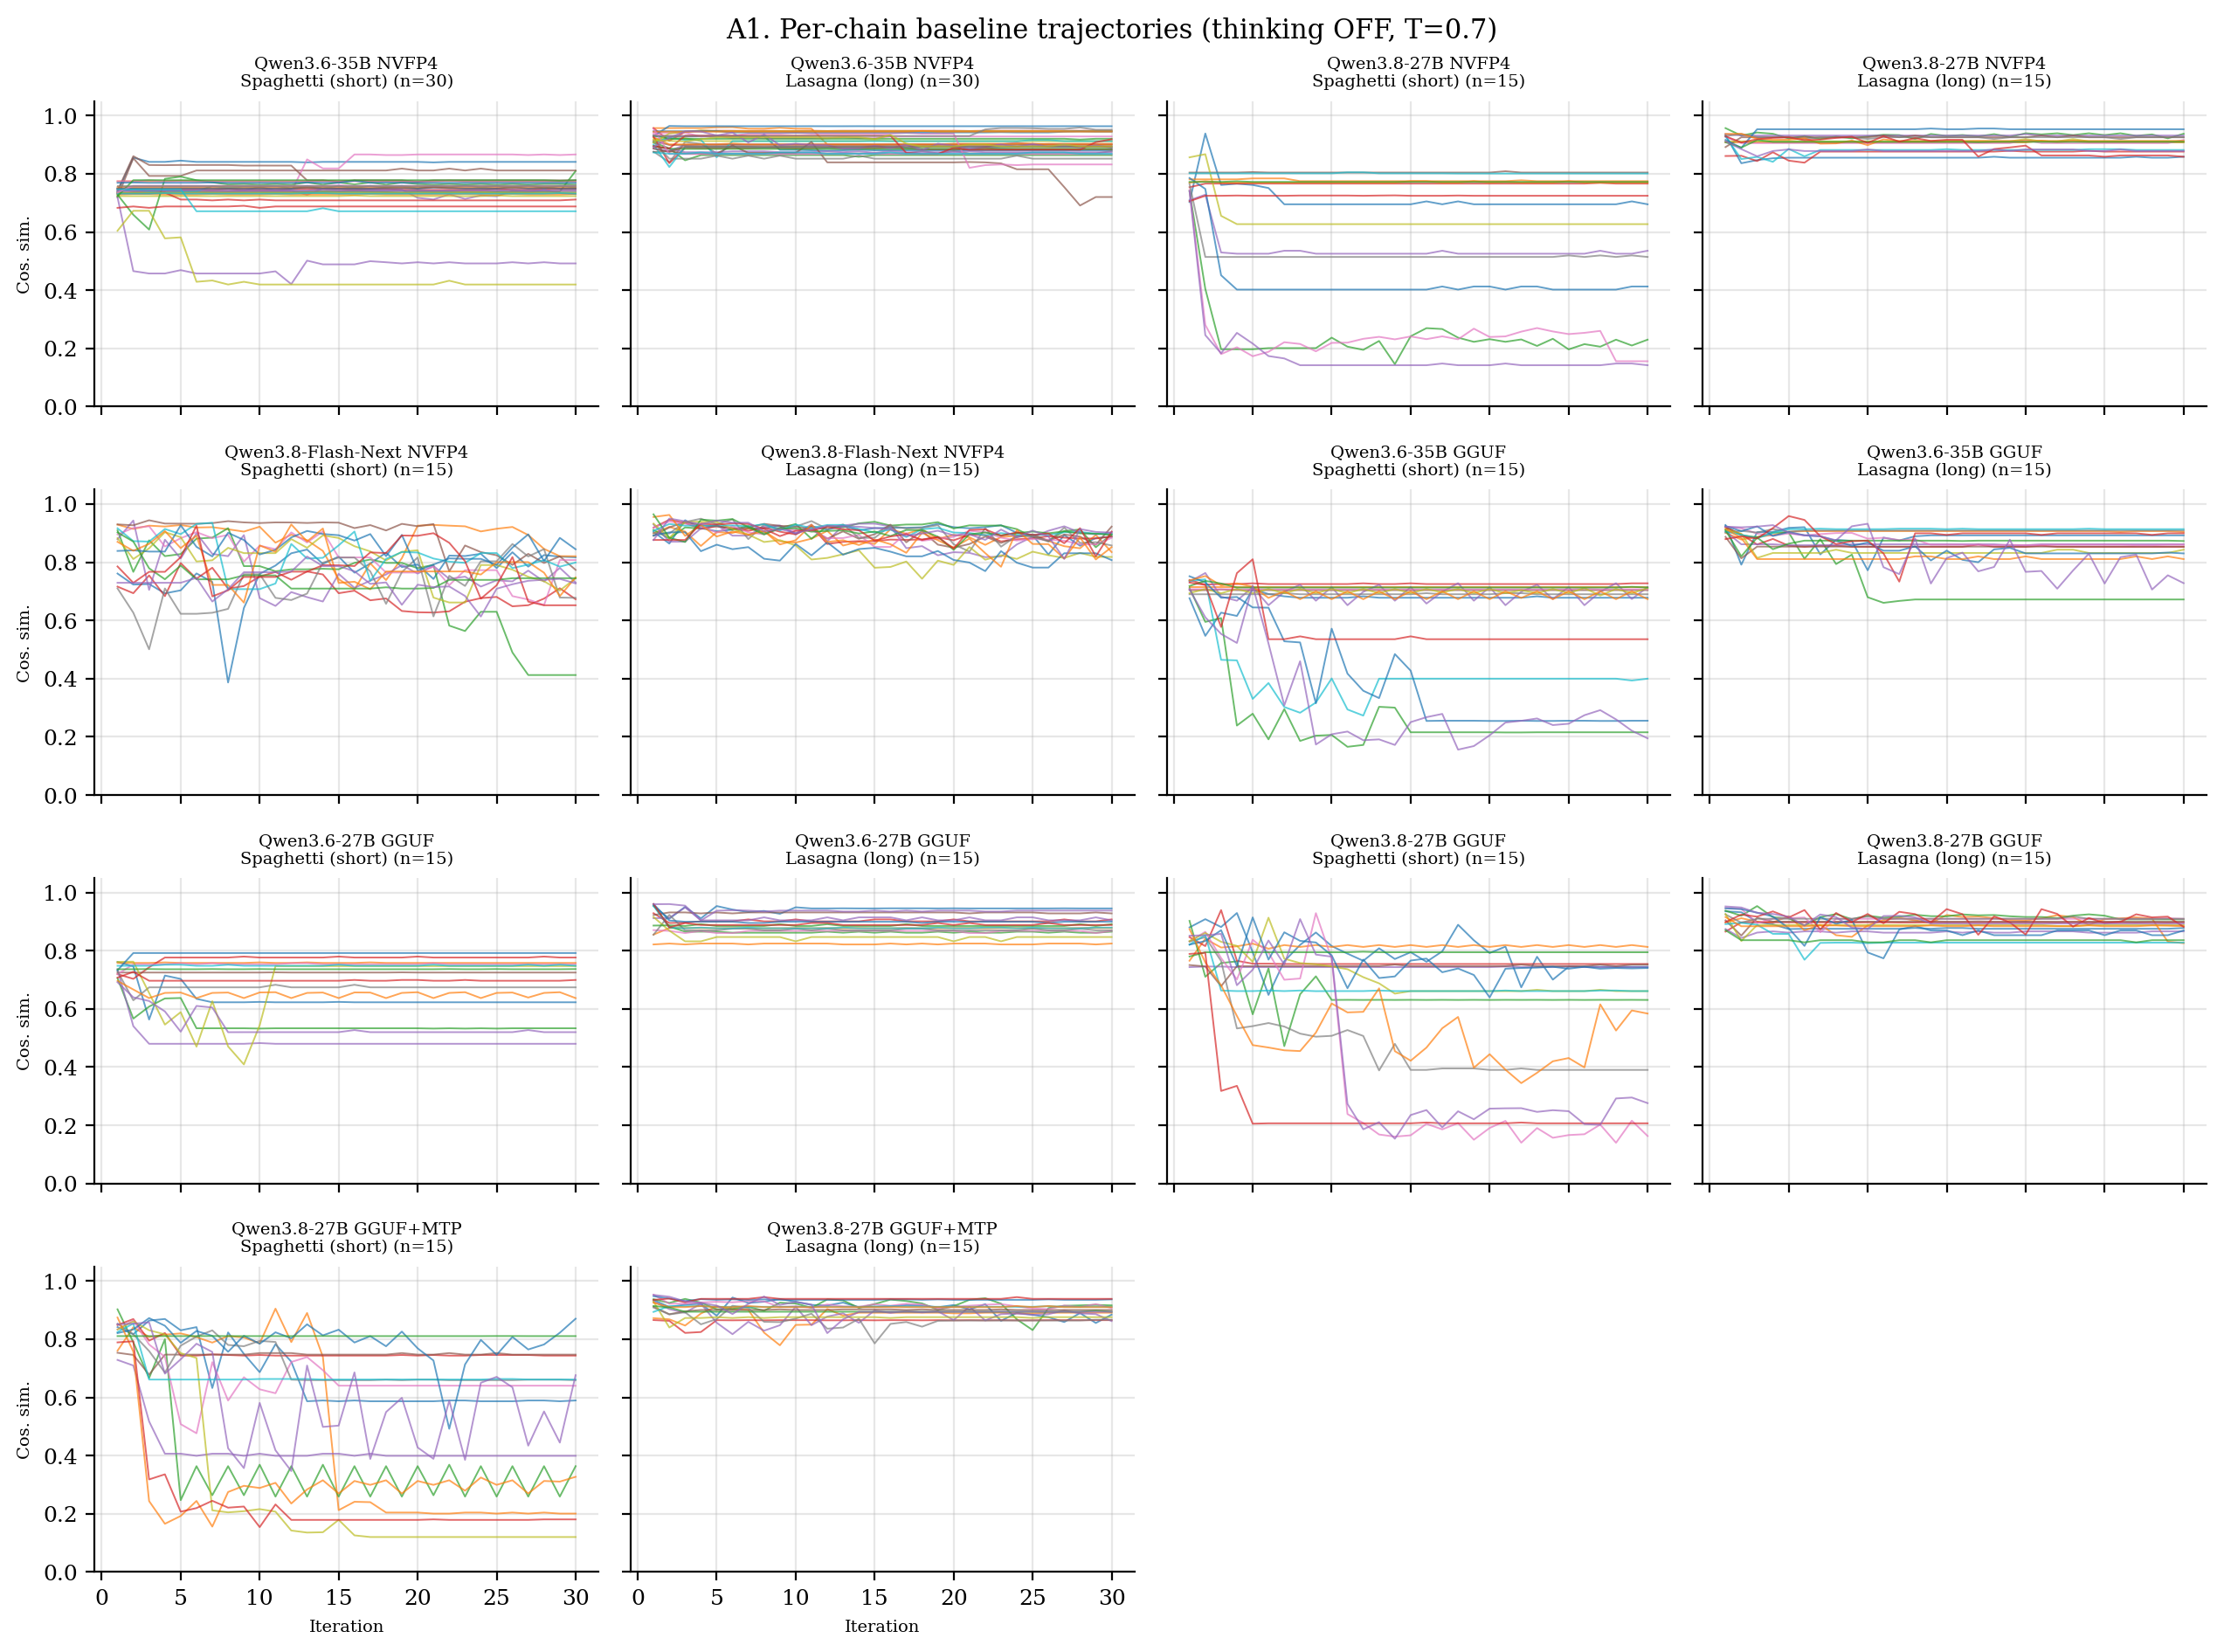
\includegraphics[width=\textwidth,height=0.4\textheight,keepaspectratio]{../results/paper3_figures/figA1_baseline_per_chain.png}
\caption{Per-chain baseline trajectories for every configuration.}
\end{figure}

\begin{figure}[htbp]
\centering
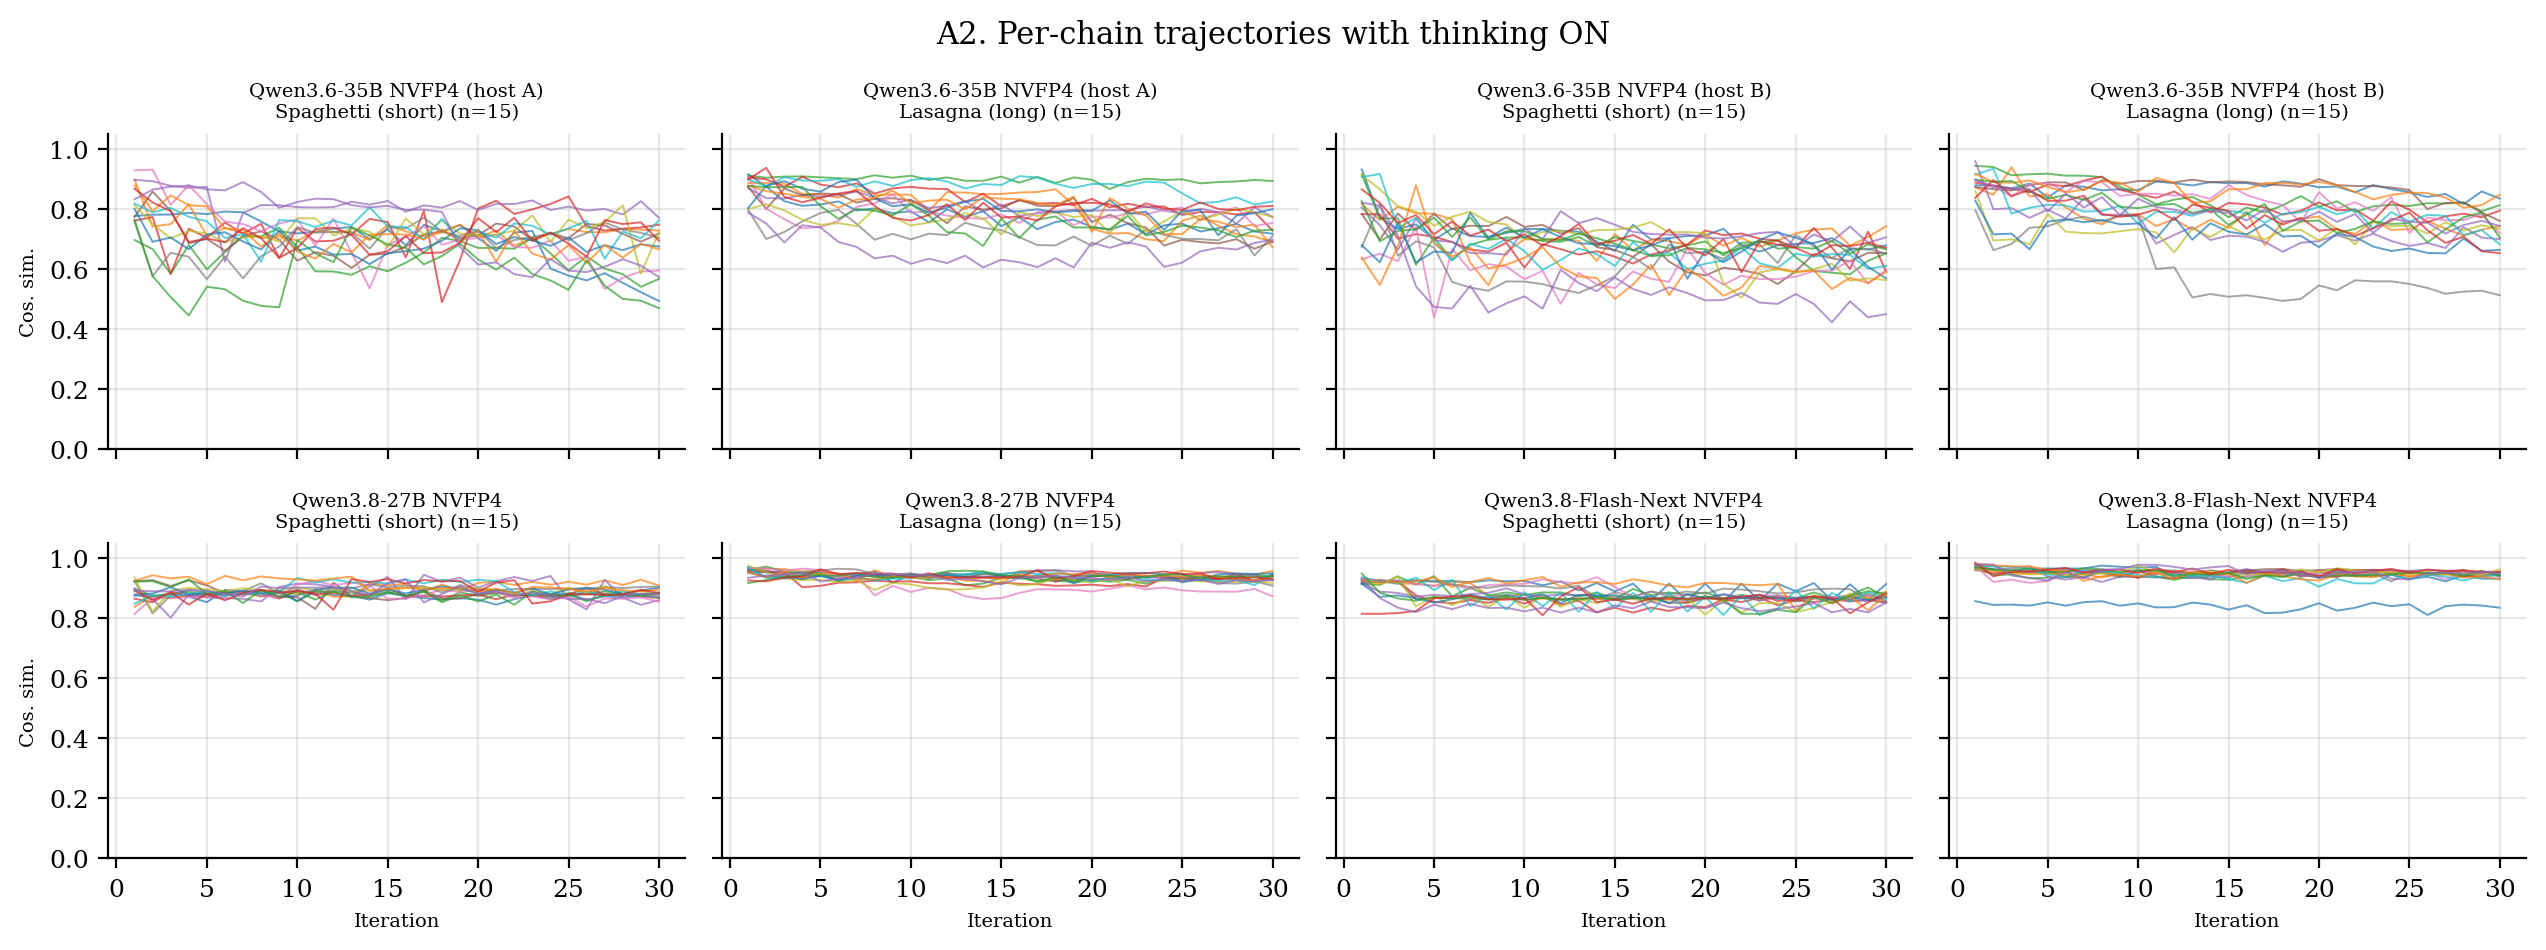
\includegraphics[width=\textwidth,height=0.4\textheight,keepaspectratio]{../results/paper3_figures/figA2_thinking_per_chain.png}
\caption{Per-chain trajectories with thinking on.}
\end{figure}

\section{Reproducibility and compute}
\label{app:compute}

\paragraph{Hardware.}
Qwen3.6-35B NVFP4 was served by vLLM on one NVIDIA RTX~5090 (32\,GB) on
each of two machines (hosts A and B). Qwen3.8-27B NVFP4 was served by vLLM
with tensor parallelism across two NVIDIA RTX~5070~Ti (16\,GB each).
Qwen3.8-Flash-Next NVFP4 was served by SGLang on one NVIDIA RTX~PRO~6000
Blackwell (96\,GB). All GGUF builds were served by llama.cpp with tensor
splitting across two NVIDIA Quadro P5000 (16\,GB each), one model resident
at a time. Embeddings were computed by Qwen3-Embedding-0.6B served by vLLM
on an RTX~5070~Ti. The GGUF runs of Paper~A used Ollama on the RTX~PRO~6000;
the change of server and GPU generation between the two papers' GGUF arms
is part of the format-and-stack confound noted in
Section~\ref{sec:format}.

\paragraph{Software.}
vLLM (NVFP4 builds; FlashInfer MoE backend, fp8 KV cache, prefix caching,
reasoning parser \texttt{qwen3}, thinking disabled by default and enabled
per request via \texttt{chat\_template\_kwargs}), SGLang (Flash-Next;
ModelOpt FP4, reasoning parser \texttt{auto}), llama.cpp router (GGUF;
q8\_0 KV cache, reasoning off; \texttt{draft-mtp} with draft length 2 for
the MTP arm). The generation budget was 16{,}384 tokens and the request
timeout 600\,s throughout.

\paragraph{Scale.}
2{,}717 chains, 87{,}110 model calls, run between 6 and 7 September 2026;
the Blackwell-hosted conditions completed in under 24 hours of wall-clock
time and the llama.cpp conditions in a further 16 hours.

\paragraph{Availability.}
The runner, the analysis script that produces every figure and table here,
the prompt files with their anchors, and the full per-iteration chain
texts are at \url{https://github.com/jhsmith409/telephone-semantic-drift},
with the chain data attached to the repository's data release as a
checksummed archive.

\end{document}
